
\documentclass[12pt,letterpaper]{article}
\usepackage[spanish,es-nodecimaldot]{babel}
\usepackage[utf8]{inputenc}
\usepackage[T1]{fontenc}
\usepackage{lmodern}
\usepackage{amsmath,amssymb,booktabs,geometry,graphicx,float,siunitx,longtable,array}
\usepackage{mathtools,enumitem,listings,xcolor,caption}
\usepackage[hidelinks]{hyperref}
\newcommand{\gam}{1.4}
\newcommand{\Rgas}{287}
\newcommand{\pu}{300}
\newcommand{\Tu}{300}
\newcommand{\hth}{0.025}
\newcommand{\heh}{0.040}
\newcommand{\hih}{0.075}
\newcommand{\Lcc}{0.25}
\newcommand{\Ldd}{0.20}
\newcommand{\dzz}{0.01}
\newcommand{\kk}{0.2}
\newcommand{\ARr}{1.6}
\newcommand{\MeSup}{1.935258}
\newcommand{\MeSub}{0.396979}
\newcommand{\peSup}{0.141318}
\newcommand{\TeSup}{0.571741}
\newcommand{\peSupPa}{42.395}
\newcommand{\TeSupK}{171.52}
\newcommand{\VeSup}{508.0}
\newcommand{\aeSup}{262.5}
\newcommand{\peSubr}{0.897079}
\newcommand{\TeSubr}{0.969445}
\newcommand{\mdotsemi}{0.17502}
\newcommand{\mdotfull}{0.35003}
\newcommand{\rhostar}{2.2088}
\newcommand{\astar}{316.94}
\newcommand{\rhocero}{3.4843}
\newcommand{\coefm}{0.002334}
\newcommand{\pbSubLim}{0.8971}
\newcommand{\pbShockExit}{0.5939}
\newcommand{\pbAdapt}{0.1413}
\newcommand{\pbSubLimkPa}{269.1}
\newcommand{\pbShockExitkPa}{178.2}
\newcommand{\pbAdaptkPa}{42.4}
\newcommand{\pIIs}{4.2028}
\newcommand{\sgExit}{0.7510}
\newcommand{\pBS}{276}
\newcommand{\pBSr}{0.9200}
\newcommand{\MeS}{0.34720}
\newcommand{\AeAsS}{1.79027}
\newcommand{\AtAsS}{1.11892}
\newcommand{\MtS}{0.66878}
\newcommand{\mdotS}{0.15642}
\newcommand{\TeS}{292.94}
\newcommand{\VeS}{119.12}
\newcommand{\AsAtS}{0.89372}
\newcommand{\MsI}{1.814789}
\newcommand{\MsII}{0.613228}
\newcommand{\AsAt}{1.455216}
\newcommand{\xsC}{0.13462}
\newcommand{\xsLd}{0.67309}
\newcommand{\pIIpI}{3.67570}
\newcommand{\rrC}{2.38269}
\newcommand{\pdospu}{0.806095}
\newcommand{\MeC}{0.528013}
\newcommand{\TeC}{284.16}
\newcommand{\VeC}{178.41}
\newcommand{\pBC}{200}
\newcommand{\pBCr}{0.66667}
\newcommand{\pdos}{241.829}
\newcommand{\AstarC}{1.24055}
\newcommand{\AeAstarC}{1.28975}
\newcommand{\TIIT}{1.54267}
\newcommand{\hxs}{0.036380}
\newcommand{\pIkPa}{51.044}
\newcommand{\pIIkPa}{187.621}
\newcommand{\pIrel}{0.17015}
\newcommand{\TIK}{180.87}
\newcommand{\TIIK}{279.02}
\newcommand{\MsDen}{3.31738}
\newcommand{\nbis}{40}
\newcommand{\xAs}{0.10}
\newcommand{\hAs}{0.03250}
\newcommand{\aAs}{1.30000}
\newcommand{\MAs}{1.658848}
\newcommand{\pAs}{0.215522}
\newcommand{\TAs}{0.645013}
\newcommand{\pAsPa}{64.656}
\newcommand{\TAsK}{193.50}
\newcommand{\xBs}{-0.10}
\newcommand{\hBs}{0.042275}
\newcommand{\aBs}{1.690983}
\newcommand{\MBs}{0.371330}
\newcommand{\pBs}{0.909179}
\newcommand{\TBs}{0.973163}
\newcommand{\cosA}{0.0}
\newcommand{\MtrialA}{1.5}
\newcommand{\rTr}{1.862069}
\newcommand{\PiTr}{2.458333}
\newcommand{\MIITr}{0.701089}
\newcommand{\sgTr}{0.929787}
\newcommand{\AeAdosTr}{1.487658}
\newcommand{\MeTr}{0.434822}
\newcommand{\prTr}{0.878176}
\newcommand{\FTr}{+0.149850}
\newcommand{\pBeTr}{0.816516}
\newcommand{\rpow}{8.810188}
\newcommand{\Pipow}{0.105535}
\newcommand{\FaExt}{+0.23041}
\newcommand{\FbExt}{-0.07274}
\newcommand{\rpowC}{20.880350}
\newcommand{\PipowC}{0.038605}
\newcommand{\PiCnum}{2.675704}
\newcommand{\MsCsq}{3.293461}
\newcommand{\numMdos}{3.317384}
\newcommand{\denMdos}{8.821690}
\newcommand{\MeShock}{1.935258}

\geometry{margin=2.5cm}
\sisetup{output-decimal-marker={.}}
\numberwithin{equation}{section}

\begin{document}
% ==========================================
% PORTADA - UNIVERSIDAD AUTÓNOMA DE CHIHUAHUA
% ==========================================
\begin{titlepage}
\centering
\thispagestyle{empty}
% Logotipo institucional
\begin{center}
    \includegraphics[width=4cm]{logo_uach.png}
\end{center}
\vspace{0.5cm}
% Universidad
{\LARGE\bfseries
Universidad Autónoma de\\
Chihuahua\par}
\vspace{0.5cm}
{\Large\bfseries
Facultad de Ingeniería\par}
\vspace{1.6cm}
% Título del proyecto
{\LARGE\bfseries
Proyecto Final:\par}
\vspace{0.3cm}
{\LARGE\bfseries
Análisis Computacional de Flujo\\
Compresible en Toberas\par}
\vspace{1.2cm}
% Materia
{\Large\bfseries
Aerodinámica II\par}
\vspace{1.3cm}
% Integrantes
{\normalsize\bfseries
Integrantes del equipo:\par}
\vspace{0.3cm}
\begin{tabular}{ll}
Sandra Valeria Tarango Melendez &
Matrícula: 365216 \\
Karyme Hernandez Teran &
Matrícula: 360725
\end{tabular}
\par
\vspace{0.9cm}
% Profesor
{\normalsize
\textbf{Profesor:} M.Sc. Carlos Alberto Molina Holguín\par}
\vspace{0.4cm}
% Fecha de entrega
{\normalsize
\textbf{Fecha de entrega:} 22 de Noviembre de 2026\par}
\vspace{0.4cm}
{\normalsize
\textbf{Grupo:} 9A1\par}
\vspace{0.4cm}
{\normalsize
\textbf{Nivel presentado:} Nivel 1\par}
\vfill
\end{titlepage}
% ==========================================
% FIN DE PORTADA
% ==========================================
\tableofcontents
% ==========================================
% ABSTRACT
% ==========================================
\newpage
\section*{Resumen}
\addcontentsline{toc}{section}{Resumen}
Se estudió numéricamente el flujo compresible no viscoso en una tobera convergente-divergente plana (relación de áreas 1.6) y se comparó con un modelo cuasiunidimensional que usa el área real. Con Gmsh se generaron mallas estructuradas de 2 600, 10 400 y 41 600 celdas y con OpenFOAM-8 (rhoCentralFoam) se resolvieron las ecuaciones de Euler en tres regímenes: subsónico no estrangulado (contrapresión de 276 kPa), supersónico adaptado y con choque normal interno (200 kPa). Con número de Courant de 0.1, el error medio del número de Mach fue de 0.08 a 0.22~\%, el del gasto másico de 0.02 a 0.10~\% y el balance de masa cerró dentro de 0.005~\%. El choque quedó a 0.30 a 0.36~\% de la longitud del divergente de su posición teórica, con poca sensibilidad a la malla, aunque sin demostrar convergencia rigurosa. Con Courant de 0.3 a 0.5, el error del gasto subsónico llegó a 13~\% y el choque se desplazó de 6 a 9~\% de esa longitud: el paso de tiempo fue el parámetro más influyente. El modelo reproduce la teoría dentro de 0.4~\% con Courant 0.1; el error restante puede deberse a la discretización o a las diferencias entre modelos.

\vspace{0.3cm}
\noindent\textbf{Palabras clave:} flujo compresible, tobera convergente-divergente, dinámica de fluidos computacional (CFD), número de Mach, onda de choque normal, OpenFOAM, número de Courant.

\newpage
\section*{Abstract}
\addcontentsline{toc}{section}{Abstract}
Inviscid compressible flow in a planar convergent-divergent nozzle (area ratio 1.6) was studied numerically and compared with a quasi-one-dimensional model that uses the real area distribution. Structured meshes of 2,600, 10,400 and 41,600 cells were generated with Gmsh, and the Euler equations were solved with OpenFOAM-8 (rhoCentralFoam) for three regimes: unchoked subsonic flow (back pressure of 276 kPa), ideally expanded supersonic flow, and supersonic flow with an internal normal shock (200 kPa). Results were averaged in time and by cross section. With a Courant number of 0.1, the mean Mach number error was 0.08 to 0.22~\%, the mass-flow error 0.02 to 0.10~\%, and the mass balance closed within 0.005~\%. The shock position was within 0.30 to 0.36~\% of the divergent length of the theoretical value, with low mesh sensitivity, although rigorous mesh convergence was not demonstrated. With Courant numbers of 0.3 to 0.5, the subsonic mass-flow error reached 13~\% and the shock moved 6 to 9~\% of that length: the time step was the most influential parameter. The model reproduces the theory within 0.4~\% at Courant 0.1; the remaining error may come from discretization or from model differences.

\vspace{0.3cm}
\noindent\textbf{Keywords:} compressible flow, convergent-divergent nozzle, computational fluid dynamics (CFD), Mach number, normal shock wave, OpenFOAM, Courant number.
\newpage
\section{Introducción}
El estudio del flujo compresible constituye una parte fundamental de la aerodinámica, especialmente en aplicaciones donde los fluidos alcanzan velocidades elevadas y experimentan variaciones significativas de presión, temperatura y densidad. Este comportamiento se presenta en diversos sistemas de ingeniería aeroespacial, como motores de reacción, sistemas de propulsión de cohetes y dispositivos de expansión de gases, en los cuales resulta indispensable comprender la relación entre las condiciones de operación y las propiedades del flujo.

Dentro de estos sistemas, las toberas convergentes-divergentes desempeñan un papel importante debido a su capacidad para acelerar un fluido mediante cambios controlados en el área transversal. Su funcionamiento se basa en la transformación de energía térmica y de presión en energía cinética, permitiendo que, bajo determinadas condiciones, el flujo alcance velocidades sónicas en la garganta y posteriormente supersónicas en la sección divergente. Sin embargo, el comportamiento del fluido no depende únicamente de la geometría, sino también de las condiciones de alimentación y de la presión existente a la salida, conocida como contrapresión.

La variación de la contrapresión puede provocar diferentes regímenes de operación, desde un flujo completamente subsónico hasta condiciones supersónicas con formación de ondas de choque. Estos fenómenos producen cambios importantes en la distribución de presión, temperatura, velocidad y número de Mach, por lo que su estudio resulta necesario para comprender el desempeño de una tobera y las limitaciones de sus condiciones de funcionamiento.

\subsection{Alcance y pregunta del estudio}

Este reporte corresponde al \textbf{Nivel 1} del proyecto: tobera plana de dos dimensiones con relación de áreas $A_e/A_t=1.6$, resuelta como semidominio con flujo inviscido y compresible, en tres regímenes internos (subsónico no estrangulado, supersónico adaptado y con choque normal interno) y con tres resoluciones de malla en el caso con choque. La comparación se hace con la teoría cuasiunidimensional que usa la distribución real de áreas $A(x)$ de la geometría. El trabajo responde a la pregunta: \emph{¿con qué precisión reproduce una simulación con \texttt{rhoCentralFoam} la solución cuasiunidimensional de cada régimen, y cómo dependen los resultados de la malla y del paso de tiempo?}

\newpage
\section{Objetivos}
\subsection{Objetivo general}
Analizar el comportamiento del flujo compresible a través de una
tobera convergente-divergente mediante herramientas de dinámica
de fluidos computacional (CFD), utilizando Gmsh para la
generación de la geometría y las mallas, OpenFOAM para la
resolución numérica y Python (NumPy y Matplotlib) para el posprocesamiento,
con la finalidad de estudiar diferentes regímenes de
operación, evaluar la sensibilidad de los resultados al
refinamiento de malla y comparar las predicciones numéricas
con un modelo analítico cuasiunidimensional.

\subsection{Objetivos específicos}
\begin{itemize}
\item Construir una geometría bidimensional de una
    tobera convergente-divergente con una relación de
    áreas $A_e/A_t = 1.6$, utilizando perfiles
    cosenoidales para representar las secciones
    convergente y divergente.

    \item Generar tres mallas estructuradas de diferentes
    resoluciones mediante Gmsh, manteniendo las mismas
    características geométricas para realizar un
    estudio de sensibilidad de malla.

    \item Configurar el solver \texttt{rhoCentralFoam}
    en OpenFOAM 8, estableciendo las propiedades
    termodinámicas del aire, las condiciones iniciales
    y de frontera, así como los parámetros necesarios
    para la simulación del flujo compresible.

    \item Estudiar tres regímenes de operación de la
    tobera: flujo subsónico no estrangulado, flujo
    supersónico adaptado y flujo con presencia de
    una onda de choque normal en la región divergente.

    \item Analizar la distribución del número de Mach,
    presión, temperatura y velocidad a lo largo de
    la tobera, identificando los cambios asociados
    con cada régimen de funcionamiento.

    \item Evaluar la influencia del refinamiento de
    malla sobre el gasto másico, la localización de
    la onda de choque y las propiedades del flujo
    antes y después de esta.

    \item Comparar los resultados numéricos con las
    predicciones del modelo analítico cuasiunidimensional,
    utilizando las relaciones isentrópicas, la ecuación
    área--Mach y las relaciones de choque normal.
\end{itemize}
\newpage
\section{Hipótesis del modelo cuasiunidimensional}

Para desarrollar el análisis teórico del flujo compresible
en la tobera convergente-divergente, se establecieron las
siguientes hipótesis simplificadoras. Estas permiten aplicar
las ecuaciones de conservación y las relaciones del flujo
compresible, obteniendo una solución analítica de referencia
para su posterior comparación con los resultados CFD.

\begin{enumerate}

    \item \textbf{Flujo cuasiunidimensional:}
    Se considera que las propiedades del fluido, como
    presión, temperatura, densidad y velocidad, varían
    principalmente en la dirección longitudinal $x$.
    Se supone que estas propiedades son uniformes en
    cada sección transversal de la tobera.

    \item \textbf{Flujo estacionario:}
    Se supone que las propiedades del flujo no cambian
    con el tiempo, permitiendo analizar únicamente
    sus variaciones espaciales. Esta condición se
    aplica al modelo analítico, mientras que las
    simulaciones CFD se desarrollan inicialmente
    mediante un enfoque transitorio.

    \item \textbf{Gas perfecto y calóricamente perfecto:}
    El aire se modela mediante la ecuación de estado:

    \begin{equation}
        p = \rho RT
    \end{equation}

    Considerando constantes las propiedades
    $\gamma = 1.4$ y
    $R = 287\ \mathrm{J/(kg\cdot K)}$.

    \item \textbf{Flujo adiabático e inviscido:}
    Se desprecia la transferencia de calor con las
    paredes y los efectos de fricción. Por lo tanto,
    el modelo considera paredes impermeables y
    deslizantes, sin pérdidas viscosas.

    \item \textbf{Flujo isentrópico excepto en el choque:}
    Se considera que el flujo es isentrópico en las
    regiones sin discontinuidades. Cuando aparece
    una onda de choque normal, aumenta la entropía
    y disminuye la presión total:

    \begin{equation}
        p_{02} < p_{01}
    \end{equation}

    \item \textbf{Dominio bidimensional planar:}
    Se modela únicamente la mitad superior de la
    tobera debido a su simetría, considerando una
    profundidad constante de $b = 0.01$ m.
    La relación de áreas se expresa como:

    \begin{equation}
        \frac{A(x)}{A_t} = \frac{h(x)}{h_t}
    \end{equation}

    \item \textbf{Condiciones de alimentación:}
    Se supone que el flujo proviene de un reservorio
    con condiciones totales constantes:

    \begin{equation}
        p_{01} = 300\ \mathrm{kPa},
        \qquad T_{01} = 300\ \mathrm{K}
    \end{equation}

    Estas condiciones se utilizan como referencia
    para analizar los distintos regímenes de operación.

\end{enumerate}

Las hipótesis anteriores permiten simplificar el
comportamiento del flujo y establecer una base teórica
para estudiar los regímenes subsónico, supersónico
adaptado y con choque normal interno. Asimismo,
facilitan la comparación entre las predicciones
analíticas y los resultados numéricos obtenidos
mediante OpenFOAM.

\newpage
\section{Marco teórico}
\label{sec:marco}

Las relaciones del flujo compresible de esta sección (isentrópicas, área--Mach, choque normal y regímenes de la tobera) siguen la formulación de Anderson~\cite{anderson2003,anderson2017}; los fundamentos numéricos se apoyan en Kurganov y colaboradores~\cite{kurganov2000,kurganov2001}, en la implementación de \texttt{rhoCentralFoam}~\cite{greenshields2010}, en el limitador de van Leer~\cite{vanleer1979} y en la condición de Courant--Friedrichs--Lewy~\cite{cfl1928}.

\subsection{Fundamentos del flujo compresible y gases ideales}

La compresibilidad es la capacidad de un fluido para experimentar
cambios en su densidad como consecuencia de variaciones de presión
y temperatura. En el caso de los gases, este fenómeno adquiere
especial importancia cuando el fluido alcanza velocidades
elevadas, ya que las variaciones de densidad influyen directamente
en su comportamiento aerodinámico.

Como criterio práctico, cuando el número de Mach es inferior
a 0.3, los efectos de compresibilidad asociados con la velocidad
suelen ser pequeños y, en determinadas condiciones, pueden
despreciarse. Sin embargo, para valores de Mach superiores
a 0.3, generalmente es necesario considerar las variaciones
de densidad en el análisis del flujo.

Este comportamiento es especialmente relevante en las toberas
convergentes-divergentes, donde la aceleración del fluido produce
cambios importantes en la presión, temperatura y densidad.

\begin{figure}[htbp]
    \centering
    \includegraphics[width=0.5\textwidth]
    {fig01_flujo_compresible.png}
    \caption{Comparación entre flujo compresible e
    incompresible.}
    \label{fig:flujo_compresible}
\end{figure}

Para describir las propiedades termodinámicas del aire,
se utiliza el modelo de gas ideal, cuya ecuación de
estado es:

\begin{equation}
    p=\rho RT
\end{equation}

donde $p$ representa la presión estática (Pa),
$\rho$ la densidad (kg/m$^3$), $R$ la constante
específica del gas (J/(kg K)) y $T$ la temperatura
estática (K).

En este proyecto, el aire se considera un gas
calóricamente perfecto, por lo que sus calores
específicos a presión constante ($c_p$) y a
volumen constante ($c_v$) se mantienen constantes.

La relación entre ambos se expresa mediante
la razón de calores específicos:

\begin{equation}
    \gamma=\frac{c_p}{c_v}
\end{equation}

Asimismo, para un gas ideal se cumple:

\begin{equation}
    R=c_p-c_v
\end{equation}

Para el aire se adoptan los siguientes valores:

\begin{equation}
    \gamma=1.4,
    \qquad
    R=287\ \mathrm{J/(kg\cdot K)}
\end{equation}

A partir de estas propiedades, el calor específico
a presión constante se determina como:

\begin{equation}
    c_p=\frac{\gamma R}{\gamma-1}
    =1004.5\ \mathrm{J/(kg\cdot K)}
\end{equation}

Estas propiedades permiten relacionar las variables
termodinámicas y estudiar los cambios de estado
que experimenta el aire durante su paso por la tobera.

Para un flujo estacionario cuasiunidimensional,
la ecuación de continuidad establece que el
gasto másico permanece constante:

\begin{equation}
    \dot{m}=\rho AV=\mathrm{constante}
\end{equation}

donde $\dot{m}$ es el gasto másico (kg/s),
$A$ el área transversal (m$^2$) y $V$
la velocidad del fluido (m/s).

Por otra parte, considerando un flujo estacionario,
adiabático, sin trabajo de eje y con cambios
despreciables de energía potencial, la ecuación
de conservación de energía se expresa como:

\begin{equation}
    h+\frac{V^2}{2}=h_0
\end{equation}

Para un gas calóricamente perfecto:

\begin{equation}
    c_pT+\frac{V^2}{2}=c_pT_0
\end{equation}

Esta relación indica que, a medida que el fluido
aumenta su velocidad, su temperatura estática
disminuye. Bajo estas hipótesis, la temperatura
total permanece constante, incluso cuando se
presenta una onda de choque normal adiabática,
aunque la presión total disminuye debido a
las irreversibilidades del proceso.


\subsection{Número de Mach y clasificación de los regímenes de flujo}

El número de Mach es un parámetro adimensional
que permite identificar el régimen de movimiento
de un fluido compresible. Se define como la
relación entre la velocidad local del flujo
y la velocidad local del sonido:

\begin{equation}
    M=\frac{V}{a}
\end{equation}

donde $M$ es el número de Mach, $V$ la
velocidad del fluido y $a$ la velocidad
local del sonido.

Para un gas ideal calóricamente perfecto,
la velocidad del sonido se calcula mediante:

\begin{equation}
    a=\sqrt{\gamma RT}
\end{equation}

Esta expresión muestra que la velocidad
del sonido depende de la temperatura
del gas y de sus propiedades termodinámicas.

De acuerdo con el número de Mach, el flujo
se clasifica principalmente en tres regímenes:

\begin{itemize}

    \item \textbf{Flujo subsónico ($M<1$):}
    La velocidad del fluido es menor que
    la velocidad local del sonido.

    \item \textbf{Flujo sónico ($M=1$):}
    La velocidad del fluido es igual a
    la velocidad local del sonido.
    Esta condición puede presentarse
    en la garganta de una tobera cuando
    el flujo alcanza el estrangulamiento.

    \item \textbf{Flujo supersónico ($M>1$):}
    La velocidad del fluido supera la
    velocidad local del sonido y pueden
    presentarse fenómenos como ondas
    de choque y expansiones.

\end{itemize}

\begin{figure}[htbp]
    \centering
    \includegraphics[width=0.82\textwidth]
    {fig02_regimenes_mach.png}
    \caption{Clasificación de los regímenes del
    flujo de acuerdo con el número de Mach.}
    \label{fig:regimenes_mach}
\end{figure}

Una característica fundamental del flujo
compresible es que los regímenes subsónico
y supersónico responden de manera opuesta
ante los cambios de área de un conducto.

Para un flujo cuasiunidimensional,
estacionario, inviscido e isentrópico,
esta relación se describe mediante:

\begin{equation}
    \frac{dA}{A}=(M^2-1)\frac{dV}{V}
\end{equation}

Esta ecuación permite explicar el comportamiento
del fluido en una tobera convergente-divergente.

Cuando el flujo es subsónico ($M<1$),
una disminución del área transversal
produce un aumento de velocidad, mientras
que un aumento del área provoca su
desaceleración.

En cambio, cuando el flujo es supersónico
($M>1$), ocurre lo contrario: el fluido
se acelera al aumentar el área y se
desacelera cuando esta disminuye.

Por esta razón, una tobera
convergente-divergente puede acelerar
un flujo inicialmente subsónico hasta
alcanzar $M=1$ en la garganta y,
si las condiciones de presión lo permiten,
continuar acelerándolo a velocidades
supersónicas en la sección divergente.

Este comportamiento constituye la base
del funcionamiento de la tobera estudiada
y permite comprender los diferentes
regímenes de operación que se analizarán
mediante el modelo teórico y las
simulaciones CFD.


\subsection{Condiciones de estancamiento (totales)}

Las condiciones de estancamiento, también conocidas como
propiedades totales o de remanso, representan el estado
que alcanzaría un fluido si se desacelerara hasta una
velocidad nula mediante un proceso adiabático y reversible.

Estas propiedades se identifican mediante el subíndice
$0$ e incluyen la temperatura total ($T_0$), la presión
total ($p_0$) y la densidad total ($\rho_0$).

Físicamente, las condiciones de estancamiento permiten
representar la energía del fluido considerando tanto
su estado termodinámico como su movimiento. Son
especialmente importantes en el análisis de toberas,
ya que permiten estudiar la transformación de energía
térmica en energía cinética durante la aceleración
del gas.

\subsubsection{Temperatura, presión y densidad totales}

La temperatura total representa la temperatura que
alcanzaría el fluido al detenerse adiabáticamente,
sin realizar trabajo de eje. Para un gas
calóricamente perfecto se expresa como:

\begin{equation}
    T_0=T+\frac{V^2}{2c_p}
\end{equation}

Por otra parte, la presión y la densidad totales
corresponden a los valores que se obtendrían al
detener el fluido de manera isentrópica.

Sus relaciones con las propiedades estáticas son:

\begin{equation}
    \frac{p_0}{p}=
    \left(1+\frac{\gamma-1}{2}M^2\right)^{
    \frac{\gamma}{\gamma-1}}
\end{equation}

\begin{equation}
    \frac{\rho_0}{\rho}=
    \left(1+\frac{\gamma-1}{2}M^2\right)^{
    \frac{1}{\gamma-1}}
\end{equation}

Estas expresiones permiten relacionar las
condiciones locales del flujo con las propiedades
de referencia del reservorio.

\subsubsection{Conservación de las propiedades totales}

En un flujo estacionario, adiabático, sin trabajo
de eje y con cambios despreciables de energía
potencial, la temperatura total permanece
constante debido a la conservación de energía.

Sin embargo, la presión total solamente se
conserva cuando el flujo es isentrópico, es
decir, cuando no existen irreversibilidades.

Por esta razón, cuando aparece una onda de
choque normal, la temperatura total permanece
constante, mientras que la presión total
disminuye debido al aumento de entropía:

\begin{equation}
    T_{02}=T_{01},
    \qquad p_{02}<p_{01}
\end{equation}

Este comportamiento es fundamental para
analizar las pérdidas de presión total
en el caso de la tobera con choque interno.

\subsubsection{Presión estática, dinámica y total}

La presión estática ($p$) es la presión
termodinámica local que ejerce el fluido,
independientemente de su velocidad.

La presión dinámica ($q$) representa una
medida de la energía cinética del flujo
por unidad de volumen y se define como:

\begin{equation}
    q=\frac{1}{2}\rho V^2
\end{equation}

Por último, la presión total ($p_0$)
representa la presión que alcanzaría
el fluido al detenerse isentrópicamente.

En flujo incompresible, la relación entre
estas presiones puede escribirse como:

\begin{equation}
    p_0=p+\frac{1}{2}\rho V^2
\end{equation}

Sin embargo, para el flujo compresible
estudiado en este proyecto, la presión
total debe determinarse mediante las
relaciones isentrópicas, ya que en general
no es igual a la suma de la presión
estática y la presión dinámica.

En la tobera convergente-divergente,
estas propiedades permiten comprender
cómo la presión estática disminuye
durante la aceleración del flujo y
cómo la presencia de una onda de choque
produce una pérdida de presión total.


\subsection{Flujo isentrópico en toberas}

El flujo isentrópico constituye uno de los modelos
fundamentales de la dinámica de gases, especialmente
en el estudio de toberas convergentes-divergentes.
Estas permiten modificar la velocidad de un fluido
mediante variaciones en el área transversal,
transformando la energía asociada con la presión
y la temperatura en energía cinética.

Un proceso se considera isentrópico cuando la
entropía del fluido permanece constante. Para
ello, el proceso debe ser adiabático y reversible,
es decir, sin transferencia de calor ni
irreversibilidades asociadas con la fricción,
la disipación viscosa o las ondas de choque.

En el análisis ideal de toberas se supone que
el flujo es estacionario, cuasiunidimensional
y que el aire se comporta como un gas ideal
calóricamente perfecto. Estas hipótesis permiten
aplicar las ecuaciones de conservación y las
relaciones termodinámicas para determinar
las propiedades del fluido.

Para un gas ideal con calores específicos
constantes, las relaciones isentrópicas entre
dos estados pueden expresarse como:

\begin{equation}
    \frac{p}{\rho^\gamma}
    =\mathrm{constante}
\end{equation}

\begin{equation}
    \frac{T_2}{T_1}
    =\left(\frac{p_2}{p_1}\right)^{
    \frac{\gamma-1}{\gamma}}
\end{equation}

Estas expresiones son válidas en las regiones
donde el flujo evoluciona sin pérdidas
irreversibles importantes. Sin embargo,
no pueden aplicarse directamente a través
de una onda de choque, debido al incremento
de entropía que ocurre en dicha discontinuidad.

En una tobera convergente-divergente tipo
Laval, el flujo subsónico puede acelerarse
en la sección convergente hasta alcanzar
la condición sónica en la garganta.
Si las condiciones de operación lo permiten,
el fluido continúa acelerándose en la
sección divergente hasta alcanzar
velocidades supersónicas.

\begin{figure}[htbp]
    \centering
    \includegraphics[width=0.82\textwidth]
    {fig03_tobera_convergente_divergente.png}
    \caption{Esquema de una tobera
    convergente-divergente tipo Laval.}
    \label{fig:tobera_laval}
\end{figure}


\subsubsection{Relaciones isentrópicas en función
del número de Mach}

Las relaciones isentrópicas permiten
determinar las propiedades estáticas
del flujo a partir de las condiciones
totales y del número de Mach.

Para un gas ideal calóricamente perfecto,
la relación entre la temperatura estática
y la temperatura total es:

\begin{equation}
    \frac{T}{T_0}=
    \left(1+\frac{\gamma-1}{2}M^2\right)^{-1}
    \label{eq:relacion_temperatura}
\end{equation}

La relación entre la presión estática
y la presión total se expresa mediante:

\begin{equation}
    \frac{p}{p_0}=
    \left(1+\frac{\gamma-1}{2}M^2\right)^{
    -\frac{\gamma}{\gamma-1}}
    \label{eq:relacion_presion}
\end{equation}

Finalmente, la relación entre la densidad
estática y la densidad total es:

\begin{equation}
    \frac{\rho}{\rho_0}=
    \left(1+\frac{\gamma-1}{2}M^2\right)^{
    -\frac{1}{\gamma-1}}
    \label{eq:relacion_densidad}
\end{equation}

Estas ecuaciones muestran que, conforme
aumenta el número de Mach, la temperatura,
la presión y la densidad estáticas
disminuyen respecto a sus valores totales.

En el presente proyecto, estas relaciones
permiten construir los perfiles teóricos
de presión y temperatura a lo largo de
la tobera a partir de la distribución
del número de Mach.

Para el caso con choque normal interno,
las relaciones isentrópicas se aplican
por separado antes y después del choque,
considerando la disminución de presión
total que ocurre a través de este.


\subsubsection{Condiciones críticas y
estrangulamiento del flujo}

Las condiciones críticas corresponden
al estado en el cual la velocidad local
del fluido es igual a la velocidad
del sonido, es decir:

\begin{equation}
    M=1
\end{equation}

En una tobera convergente-divergente,
esta condición se presenta en la
garganta cuando el flujo alcanza
el estrangulamiento.

Las propiedades críticas se identifican
mediante el superíndice $*$ y se obtienen
sustituyendo $M=1$ en las relaciones
isentrópicas.

Para la temperatura crítica:

\begin{equation}
    \frac{T^*}{T_0}
    =\frac{2}{\gamma+1}
\end{equation}

Para la presión crítica:

\begin{equation}
    \frac{p^*}{p_0}
    =\left(\frac{2}{\gamma+1}\right)^{
    \frac{\gamma}{\gamma-1}}
\end{equation}

Para la densidad crítica:

\begin{equation}
    \frac{\rho^*}{\rho_0}
    =\left(\frac{2}{\gamma+1}\right)^{
    \frac{1}{\gamma-1}}
\end{equation}

Considerando aire con $\gamma=1.4$,
se obtienen las siguientes relaciones:

\begin{equation}
    \frac{T^*}{T_0}=0.8333,
    \qquad
    \frac{p^*}{p_0}=0.5283,
    \qquad
    \frac{\rho^*}{\rho_0}=0.6339
\end{equation}

Estas condiciones representan el estado
sónico del fluido y permiten determinar
las propiedades críticas de la tobera.

Cuando el flujo se estrangula, el gasto
másico alcanza su valor máximo para
las condiciones totales de alimentación
y el área de garganta establecidas.

A partir de este punto, una disminución
adicional de la contrapresión no
incrementa el gasto másico ideal,
aunque puede modificar la distribución
del número de Mach y la aparición
de ondas de choque en la sección
divergente.


\subsection{Flujo estrangulado y gasto másico máximo}
El estrangulamiento ocurre cuando una sección crítica alcanza $M=1$ y el gasto másico ya no aumenta al reducir más la presión de respaldo, manteniendo las condiciones totales de alimentación y la geometría. La relación crítica de presión para un gas ideal isentrópico es
\begin{equation}\frac{p^*}{p_0}=\left(\frac{2}{\gamma+1}\right)^{\gamma/(\gamma-1)}.\end{equation}
El gasto másico ideal puede escribirse como
\begin{equation}
\dot m=A\frac{p_0}{\sqrt{T_0}}\sqrt{\frac{\gamma}{R}}M\left(1+\frac{\gamma-1}{2}M^2\right)^{-\frac{\gamma+1}{2(\gamma-1)}}.
\end{equation}
En la sección crítica, $M=1$ y
\begin{equation}
\dot m_{\max}=A^*\frac{p_0}{\sqrt{T_0}}\sqrt{\frac{\gamma}{R}}\left(\frac{2}{\gamma+1}\right)^{\frac{\gamma+1}{2(\gamma-1)}}.
\end{equation}
Aquí $A^*$ es el área crítica asociada con las condiciones totales de ese tramo. En un flujo estrangulado ideal antes del choque, coincide con el área de garganta; después del choque se debe usar una nueva área crítica asociada con la presión total posterior.

\subsection{Relación área--Mach}
Para flujo estacionario, cuasiunidimensional e isentrópico, la combinación de continuidad, cantidad de movimiento y la definición de velocidad del sonido conduce a
\begin{equation}\frac{dA}{A}=(M^2-1)\frac{dV}{V}.\end{equation}
Por ello, para $M<1$ la aceleración requiere una reducción de área, mientras que para $M>1$ requiere un aumento de área. La relación integrada es
\begin{equation}
\frac{A}{A^*}=\frac{1}{M}\left[\frac{2}{\gamma+1}\left(1+\frac{\gamma-1}{2}M^2\right)\right]^{\frac{\gamma+1}{2(\gamma-1)}}.
\end{equation}
Para una razón $A/A^*>1$ existen una rama subsónica y otra supersónica. La elección de rama depende del régimen y de las condiciones de presión. En el proyecto se debe evaluar la distribución real $A(x)$, no sustituirla por una geometría aproximada sin justificación.

\begin{figure}[H]
    \centering
    \includegraphics[width=0.82\textwidth]{fig04_relacion_area_mach.png}
    \caption{Relación Área-Mach.}
    \label{fig:area_mach}
\end{figure}


\subsection{Tobera convergente-divergente y bloqueo}

Una tobera convergente-divergente es un dispositivo
diseñado para modificar la velocidad de un fluido
compresible mediante variaciones en el área transversal.
Su geometría está formada por tres regiones principales:
la sección convergente, la garganta y la sección divergente.

En la sección convergente, la disminución del área
provoca la aceleración del flujo subsónico, acompañada
de una reducción de presión y temperatura estáticas.
La garganta representa el área mínima de la tobera
y es donde puede alcanzarse la condición sónica
($M=1$) cuando el flujo se estrangula.

El comportamiento de la sección divergente depende
del régimen de operación. Si el flujo permanece
subsónico, el aumento del área produce una
desaceleración. En cambio, si el flujo alcanza
condiciones supersónicas, la sección divergente
permite continuar acelerándolo, disminuyendo
su presión y temperatura estáticas.

\begin{figure}[H]
    \centering
    \includegraphics[width=0.75\textwidth]
    {fig05_tobera_laval.png}
    \caption{Geometría de una tobera
    convergente-divergente y sus secciones
    principales.}
    \label{fig:geometria_tobera_cd}
\end{figure}

Para el modelo bidimensional planar utilizado
en este proyecto, la profundidad de la tobera
se considera constante. Por lo tanto, la relación
entre el área de salida y el área de garganta
puede expresarse mediante sus alturas:

\begin{equation}
    \frac{A_e}{A_t}=\frac{h_e}{h_t}
\end{equation}

donde $A_e$ y $A_t$ representan las áreas
de salida y garganta, respectivamente,
mientras que $h_e$ y $h_t$ corresponden
a sus alturas.

En el presente proyecto se considera
una relación de áreas:

\begin{equation}
    \frac{A_e}{A_t}=1.6
\end{equation}

La garganta se localiza en $x=0$ y la
longitud de la sección divergente se
representa mediante $L_d$.


\subsubsection{Bloqueo o estrangulamiento del flujo}

El bloqueo, también conocido como
estrangulamiento o \textit{choking}, ocurre
cuando el flujo alcanza la velocidad
local del sonido en la sección de área
mínima de la tobera.

Esta condición se identifica mediante:

\begin{equation}
    M_t=1
\end{equation}

El bloqueo se alcanza cuando la
contrapresión disminuye lo suficiente
para que el flujo llegue a la condición
sónica en la garganta.

Antes del estrangulamiento, una reducción
de la contrapresión permite incrementar
la velocidad y el gasto másico del fluido.

Sin embargo, una vez que la garganta
alcanza $M=1$, el gasto másico llega
a su valor máximo para las condiciones
totales de alimentación y el área
de garganta establecidas.

A partir de este punto, una disminución
adicional de la contrapresión no
incrementa el gasto másico ideal,
aunque puede modificar el comportamiento
del flujo en la sección divergente,
incluyendo la aparición o desplazamiento
de ondas de choque.

Este fenómeno ocurre porque la garganta
sónica establece una condición crítica
que limita el flujo másico que puede
atravesar la sección mínima.


\subsubsection{Gasto másico máximo o bloqueado}

Para un flujo estacionario, adiabático,
isentrópico y de gas ideal calóricamente
perfecto, el gasto másico se expresa como:

\begin{equation}
    \dot{m}=\rho AV
\end{equation}

Al combinar la ecuación de continuidad
con las relaciones isentrópicas, se obtiene:

\begin{equation}
    \dot{m}=
    \frac{p_0 A}{\sqrt{T_0}}
    \sqrt{\frac{\gamma}{R}}
    M
    \left(
    1+\frac{\gamma-1}{2}M^2
    \right)^{
    -\frac{\gamma+1}{2(\gamma-1)}
    }
\end{equation}

Cuando el flujo alcanza la condición
crítica en la garganta ($M_t=1$),
se obtiene la expresión del gasto
másico máximo:

\begin{equation}
    \boxed{
    \dot{m}_{\max}=
    A_t p_0
    \sqrt{\frac{\gamma}{RT_0}}
    \left(
    \frac{2}{\gamma+1}
    \right)^{
    \frac{\gamma+1}{2(\gamma-1)}
    }
    }
    \label{eq:gasto_masico_bloqueado}
\end{equation}

donde $A_t$ es el área de garganta,
$p_0$ la presión total de alimentación,
$T_0$ la temperatura total,
$\gamma$ la razón de calores específicos
y $R$ la constante específica del gas.

Esta ecuación demuestra que, para
un gas determinado, el gasto másico
máximo depende principalmente de
la presión total, la temperatura total
y el área mínima de la tobera.

En particular, el gasto másico máximo
aumenta al incrementar la presión total
o el área de garganta, mientras que
disminuye al aumentar la temperatura
total de alimentación.

Para el presente proyecto se consideran
las condiciones de referencia:

\begin{equation}
    p_{01}=300\ \mathrm{kPa},
    \qquad
    T_{01}=300\ \mathrm{K}
\end{equation}

Estas condiciones, junto con el área
de garganta, permiten calcular el
gasto másico máximo teórico y utilizarlo
como referencia para comparar los
resultados obtenidos mediante CFD.

\subsection{Presión estática, presión total y presión de respaldo}
La presión estática $p$ es una propiedad termodinámica local del gas. La presión total $p_0$ es la presión correspondiente a una desaceleración isentrópica hasta velocidad nula. La presión de respaldo $p_B$ representa la condición estática impuesta aguas abajo de la tobera.

En el caso ideal adaptado, la presión estática de salida supersónica coincide con la de respaldo: $p_e\simeq p_B$. En el modelo interno, la presión de salida no debe imponerse arbitrariamente cuando toda la sección de salida es supersónica; las condiciones de frontera deben respetar las características del flujo.


\subsection{Regímenes de operación según la contrapresión}

El comportamiento del flujo en una tobera
convergente-divergente depende principalmente de
la relación entre la presión de respaldo o
contrapresión ($p_b$) y la presión total de
alimentación ($p_{01}$).

Para una misma geometría y condiciones de
estancamiento, la variación de la contrapresión
permite establecer diferentes regímenes de
operación, desde un flujo completamente subsónico
hasta condiciones supersónicas con presencia
de ondas de choque.

En el presente proyecto se estudian tres
regímenes internos correspondientes al nivel 1:
subsónico no estrangulado (S), supersónico
adaptado (A) y flujo con choque normal interno
(C).

\subsubsection{Caso S: flujo subsónico no estrangulado}

En este régimen, la contrapresión es suficientemente
elevada para impedir que el flujo alcance la
velocidad del sonido en la garganta.

Por lo tanto, el número de Mach en la sección
mínima permanece por debajo de la unidad:

\begin{equation}
    M_t<1
\end{equation}

El fluido se acelera en la sección convergente
y posteriormente se desacelera en la divergente,
manteniendo un comportamiento subsónico en
toda la tobera.

Para el caso S se considera una contrapresión
de referencia de:

\begin{equation}
    p_b=276\ \mathrm{kPa}
    \qquad (p_b/p_{01}=0.92)
\end{equation}

Con esta condición, el modelo analítico predice
un número de Mach en la garganta de
$M_t=0.6688$ y de salida $M_e=0.3472$, con un gasto
de $0.15642$ kg/s para el semidominio (89.4~\% del gasto
bloqueado), por lo que no existe estrangulamiento.
Se descartó $p_b=290$ kPa ($M_t=0.372$, $M_e=0.221$) como
condición principal por su bajo número de Mach, en el que la
solución numérica es muy sensible a la pérdida de presión total
(Sección~\ref{sec:sens-dt}).

\subsubsection{Caso A: flujo supersónico adaptado}

El régimen supersónico adaptado ocurre cuando
el flujo alcanza la condición sónica en la
garganta y continúa acelerándose en la
sección divergente.

En este caso, el número de Mach en la garganta
es $M_t=1$, mientras que en la salida se
obtiene un flujo supersónico.

La condición de adaptación se presenta cuando
la presión estática de salida coincide con
la contrapresión:

\begin{equation}
    p_e=p_b
\end{equation}

Para la relación de áreas $A_e/A_t=1.6$,
el modelo analítico establece:

\begin{equation}
    M_e=1.935258
\end{equation}

\begin{equation}
    p_e=p_b=42.395\ \mathrm{kPa}
\end{equation}

Esta condición representa una expansión
supersónica ideal, sin necesidad de ajustes
de presión en la descarga.

\subsubsection{Caso C: flujo con choque normal interno}

Este régimen se presenta cuando la contrapresión
permite que el flujo alcance velocidades
supersónicas en la sección divergente, pero
es suficientemente elevada para provocar
la formación de una onda de choque normal
dentro de la tobera.

Antes del choque, el flujo es supersónico,
mientras que después de la discontinuidad
se vuelve subsónico:

\begin{equation}
    M_{s1}>1,
    \qquad
    M_{s2}<1
\end{equation}

A través del choque se produce un aumento
brusco de la presión estática y una
disminución de la velocidad y del número
de Mach.

Asimismo, debido a la naturaleza irreversible
del fenómeno, la presión total disminuye,
aunque la temperatura total permanece
constante bajo las hipótesis del modelo.

Para el caso C se considera una contrapresión
de referencia de:

\begin{equation}
    p_b=200\ \mathrm{kPa}
\end{equation}

La posición del choque depende de la
contrapresión y de la geometría de la tobera,
por lo que constituye una variable importante
para comparar el modelo analítico con
los resultados CFD.

\subsubsection{Rangos de contrapresión}

Los límites entre los diferentes regímenes
pueden determinarse mediante las relaciones
isentrópicas, la ecuación área--Mach y las
relaciones de choque normal.

Para la geometría estudiada, con
$A_e/A_t=1.6$ y $p_{01}=300$ kPa,
los rangos teóricos se presentan en
la Tabla~\ref{tab:regimenes_tobera}.

\begin{table}[htbp]
    \centering
    \caption{Regímenes de operación según
    la contrapresión para $A_e/A_t=1.6$.}
    \label{tab:regimenes_tobera}
    \renewcommand{\arraystretch}{1.3}
    \small
    \begin{tabular}{|l|c|c|}
        \hline
        \textbf{Régimen} &
        \textbf{$p_b/p_{01}$} &
        \textbf{$p_b$ (kPa)} \\
        \hline
        Subsónico (S) &
        $>0.8971$ &
        $>269.1$ \\
        \hline
        Choque interno (C) &
        $0.5939$--$0.8971$ &
        $178.2$--$269.1$ \\
        \hline
        Choque en salida &
        $0.5939$ &
        $178.2$ \\
        \hline
        Adaptado (A) &
        $0.1413$ &
        $42.4$ \\
        \hline
        Sobreexpandido &
        $0.1413$--$0.5939$ &
        $42.4$--$178.2$ \\
        \hline
        Subexpandido &
        $<0.1413$ &
        $<42.4$ \\
        \hline
    \end{tabular}
\end{table}

Estos valores corresponden a las predicciones
del modelo analítico ideal y permiten
identificar las condiciones de operación
de cada caso.

En particular, el límite superior del
régimen con choque interno corresponde
a la condición crítica en la garganta,
mientras que el límite inferior representa
una onda de choque localizada justo
en la salida de la tobera.

\subsubsection{Regímenes de descarga exterior}

Además de los tres casos internos, existen
condiciones de descarga sobreexpandida y
subexpandida, consideradas en el nivel 2
del proyecto.

El flujo se encuentra sobreexpandido cuando
la presión estática de salida es menor que
la presión del ambiente:

\begin{equation}
    p_e<p_b
\end{equation}

En cambio, el flujo está subexpandido cuando
la presión de salida es mayor que la
contrapresión:

\begin{equation}
    p_e>p_b
\end{equation}

En estas condiciones pueden desarrollarse
ondas de compresión, choques y abanicos
de expansión fuera de la tobera.

Estos fenómenos se mencionan como parte
del comportamiento general de las toberas,
pero no forman parte de los tres casos
internos considerados en el nivel 1.

Finalmente, para comparar los regímenes
S, A y C se analizarán los perfiles
de número de Mach, presión y temperatura
normalizadas, así como el gasto másico
y las propiedades del flujo en la salida.



\subsection{Ondas de choque normales}

Una onda de choque normal es una discontinuidad
aproximadamente perpendicular a la dirección del
flujo, caracterizada por cambios bruscos de presión,
temperatura, densidad y velocidad.

Este fenómeno ocurre cuando un flujo supersónico
experimenta una compresión intensa, provocando
su transición hacia un régimen subsónico.

A diferencia de una transformación isentrópica,
el choque normal es un proceso irreversible,
debido a que existe generación de entropía
y una pérdida de presión total.

Aunque las propiedades del fluido cambian
bruscamente, se mantienen las leyes de
conservación de masa, cantidad de movimiento
y energía.

\subsubsection{Ecuaciones de conservación}

Para un choque normal estacionario, adiabático
y sin trabajo externo, considerando un gas
ideal calóricamente perfecto, las ecuaciones
de conservación se expresan de la siguiente manera.

La conservación de masa establece que el
flujo másico permanece constante:

\begin{equation}
    \rho_1 V_1=\rho_2 V_2
\end{equation}

La conservación de cantidad de movimiento
relaciona los cambios de presión y velocidad:

\begin{equation}
    p_1+\rho_1 V_1^2
    =p_2+\rho_2 V_2^2
\end{equation}

Por su parte, la conservación de energía
establece que la entalpía total permanece
constante:

\begin{equation}
    h_1+\frac{V_1^2}{2}
    =h_2+\frac{V_2^2}{2}
\end{equation}

Para un gas calóricamente perfecto:

\begin{equation}
    c_pT_1+\frac{V_1^2}{2}
    =c_pT_2+\frac{V_2^2}{2}
\end{equation}

Los subíndices 1 y 2 representan las
condiciones inmediatamente antes y después
del choque, respectivamente.

Estas ecuaciones permiten obtener las
relaciones entre las propiedades del
flujo a ambos lados de la discontinuidad.


\subsubsection{Relaciones de Rankine--Hugoniot}

Las relaciones de Rankine--Hugoniot describen
los cambios de las propiedades del fluido
a través de una onda de choque normal.

Para un número de Mach incidente
$M_{s1}>1$, el número de Mach posterior
al choque se calcula mediante:

\begin{equation}
    M_{s2}^2=
    \frac{
    1+\frac{\gamma-1}{2}M_{s1}^2
    }{
    \gamma M_{s1}^2-\frac{\gamma-1}{2}
    }
\end{equation}

La relación de presiones estáticas es:

\begin{equation}
    \frac{p_2}{p_1}
    =1+\frac{2\gamma}{\gamma+1}
    \left(M_{s1}^2-1\right)
\end{equation}

La relación de densidades se expresa como:

\begin{equation}
    \frac{\rho_2}{\rho_1}
    =\frac{(\gamma+1)M_{s1}^2}{
    (\gamma-1)M_{s1}^2+2}
\end{equation}

Finalmente, la relación de temperaturas
se determina mediante:

\begin{equation}
    \frac{T_2}{T_1}
    =\frac{p_2/p_1}{\rho_2/\rho_1}
\end{equation}

Estas relaciones muestran que el flujo
se desacelera de supersónico a subsónico,
mientras que la presión, temperatura
y densidad estáticas aumentan.

\begin{figure}[H]
    \centering
    \includegraphics[width=0.75\textwidth]
    {fig06_choque_normal_tobera.png}
    \caption{Representación esquemática
    de una onda de choque normal en la
    sección divergente de una tobera.}
    \label{fig:choque_normal_tobera}
\end{figure}


\subsubsection{Pérdida de presión total
y generación de entropía}

Aunque la temperatura total se conserva
a través de un choque normal adiabático,
la presión total disminuye debido a
las irreversibilidades del proceso.

La relación entre las presiones totales
antes y después del choque se expresa como:

\begin{equation}
    \frac{p_{02}}{p_{01}}
    =\frac{p_2}{p_1}
    \left[
    \frac{
    1+\frac{\gamma-1}{2}M_{s2}^2
    }{
    1+\frac{\gamma-1}{2}M_{s1}^2
    }
    \right]^{
    \frac{\gamma}{\gamma-1}}
\end{equation}

Para un choque normal:

\begin{equation}
    p_{02}<p_{01},
    \qquad
    T_{02}=T_{01}
\end{equation}

La generación de entropía puede calcularse
mediante la relación:

\begin{equation}
    s_2-s_1
    =c_p\ln\left(\frac{T_2}{T_1}\right)
    -R\ln\left(\frac{p_2}{p_1}\right)
\end{equation}

Debido a que la temperatura total permanece
constante, esta expresión también puede
escribirse como:

\begin{equation}
    \Delta s
    =-R\ln\left(\frac{p_{02}}{p_{01}}\right)>0
\end{equation}

Por lo tanto, la disminución de presión
total representa una medida de las
pérdidas irreversibles producidas
por la onda de choque.


\subsubsection{Área crítica posterior al choque}

En una tobera con choque normal interno,
la disminución de presión total modifica
el área crítica asociada con el flujo
aguas abajo de la discontinuidad.

Como el gasto másico y la temperatura
total se conservan, se cumple:

\begin{equation}
    p_{01}A_1^*
    =p_{02}A_2^*
\end{equation}

Considerando que la garganta está
estrangulada antes del choque:

\begin{equation}
    A_1^*=A_t
\end{equation}

Se obtiene la nueva área crítica:

\begin{equation}
    \boxed{
    A_2^*=
    \frac{A_t}{p_{02}/p_{01}}
    }
    \label{eq:area_critica_postchoque}
\end{equation}

Debido a que $p_{02}/p_{01}<1$,
el área crítica posterior al choque
es mayor que el área de garganta.

Esta nueva área crítica permite
continuar el análisis isentrópico
del flujo subsónico desde el choque
hasta la salida de la tobera.

Es importante señalar que $A_2^*$
es un área crítica equivalente,
no una modificación física de la
geometría de la tobera.


\subsubsection{Determinación de la posición del choque}

La ubicación de una onda de choque normal
dentro de la sección divergente depende
de la contrapresión impuesta a la salida.

Para determinar su posición, se propone
inicialmente una ubicación $x_s$ y
se calcula el área transversal
correspondiente $A_s=A(x_s)$.

A partir de la relación área--Mach,
se determina el número de Mach
supersónico antes del choque.

Posteriormente, se aplican las
relaciones de Rankine--Hugoniot
para obtener las propiedades
posteriores y la pérdida de
presión total.

Con la nueva presión total y el
área crítica $A_2^*$, se calcula
la evolución subsónica del flujo
hasta la salida de la tobera.

La posición del choque se ajusta
hasta que la presión estática
calculada en la salida coincida
con la contrapresión establecida:

\begin{equation}
    p_e(x_s)=p_b
\end{equation}

Esta condición permite encontrar
la ubicación teórica del choque
para cada presión de respaldo.

En el presente proyecto, el caso C
considera una contrapresión de:

\begin{equation}
    p_b=200\ \mathrm{kPa}
\end{equation}

Para evaluar este régimen se
compararán la posición del choque,
las relaciones de Mach, el salto
de presión estática y la pérdida
de presión total entre el modelo
analítico y los resultados CFD.


\subsubsection{Cambios de propiedades
a través del choque}

Los principales cambios que experimenta
el fluido al atravesar una onda de
choque normal se resumen en la
Tabla~\ref{tab:propiedades_choque_normal}.

\begin{table}[H]
\centering
\caption{Cambios de propiedades a través
de una onda de choque normal.}
\label{tab:propiedades_choque_normal}
\renewcommand{\arraystretch}{1.3}
\small

\begin{tabular}{
    >{\centering\arraybackslash}p{3.0cm}
    >{\centering\arraybackslash}p{3.0cm}
    p{7.0cm}
}
\toprule
\textbf{Propiedad} &
\textbf{Cambio} &
\textbf{Interpretación física} \\
\midrule

Número de Mach &
$M_{s2}<1<M_{s1}$ &
El flujo pasa de supersónico
a subsónico. \\

Velocidad &
$V_2<V_1$ &
Disminuye la energía cinética
del flujo. \\

Presión estática &
$p_2>p_1$ &
Se produce una compresión
brusca del gas. \\

Temperatura estática &
$T_2>T_1$ &
Aumenta la energía interna
del fluido. \\

Densidad &
$\rho_2>\rho_1$ &
El gas se comprime a través
de la discontinuidad. \\

Presión total &
$p_{02}<p_{01}$ &
Existen pérdidas irreversibles
y generación de entropía. \\

Temperatura total &
$T_{02}=T_{01}$ &
Se conserva en el choque
adiabático sin trabajo externo. \\

\bottomrule
\end{tabular}
\end{table}
\newpage
\subsection{Ondas de choque oblicuas}
Las ondas de choque oblicuas aparecen cuando un flujo supersónico se desvía compresivamente, por ejemplo ante una esquina o una pared inclinada. A diferencia del choque normal, la discontinuidad forma un ángulo $\beta$ con la dirección incidente. Para un gas perfecto, el ángulo de deflexión $\theta$ satisface
\begin{equation}
\tan\theta=2\cot\beta\frac{M_1^2\sin^2\beta-1}{M_1^2(\gamma+\cos2\beta)+2}.
\end{equation}
La componente normal del número de Mach es $M_{n1}=M_1\sin\beta$ y permite aplicar las relaciones de choque normal a esa componente. Este fenómeno se incluye como contexto; el caso C del nivel 1 exige analizar principalmente un choque interno aproximadamente normal.
\begin{figure}[H]
    \centering
    \includegraphics[width=0.75\textwidth]{fig07_contornos_flujo_tobera.png}
    \caption{Representación esquemática de una tobera sobreexpandida con formación de ondas de choque oblicuas en la salida.}
    \label{fig:tobera_sobreexpandida}
\end{figure}

A través de una onda de choque oblicua, el número de Mach disminuye, la presión estática aumenta, la temperatura aumenta y la dirección del flujo cambia. Sin embar-go, dependiendo de la intensidad del choque, el flujo aguas abajo puede permanecer supersónico o volverse subsónico.


% ==========================================
% TABLA 3 - ONDAS DE CHOQUE OBLICUAS
% ==========================================
\begin{table}[H]
\centering
\caption{Características principales de las ondas de choque oblicuas en una tobera sobreexpandida.}
\label{tab:choque_oblicuo}
\renewcommand{\arraystretch}{1.3}
\small
\begin{tabular}{
>{\centering\arraybackslash}p{3.0cm}
>{\centering\arraybackslash}p{2.5cm}
p{7.2cm}
}
\toprule
\textbf{Aspecto} &
\textbf{Condición} &
\textbf{Interpretación física} \\
\midrule
Régimen de flujo &
$M_1 > 1$ &
Las ondas de choque oblicuas solo se forman
en flujo supersónico. \\
Condición de presión &
$P_e < P_b$ &
El flujo sale con presión menor que la
ambiente y necesita comprimirse. \\
Presión estática &
$P_2 > P_1$ &
La compresión a través del choque
incrementa la presión del flujo. \\
Número de Mach &
$M_2 < M_1$ &
El flujo se desacelera al cruzar
el choque oblicuo. \\
Dirección del flujo &
$\theta \neq 0$ &
El flujo cambia de dirección debido
a la deflexión producida por el choque. \\
Presión total &
$P_{02} < P_{01}$ &
Existen pérdidas irreversibles
asociadas al choque. \\
\bottomrule
\end{tabular}
\end{table}

\subsection{Expansiones de Prandtl--Meyer}
Un flujo supersónico que gira alrededor de una esquina convexa puede expandirse mediante un abanico de ondas de expansión. En el modelo ideal, la expansión es isentrópica y el número de Mach aumenta mientras la presión y la temperatura estáticas disminuyen. La función de Prandtl--Meyer es
\begin{equation}
\nu(M)=\sqrt{\frac{\gamma+1}{\gamma-1}}\tan^{-1}\sqrt{\frac{\gamma-1}{\gamma+1}(M^2-1)}-\tan^{-1}\sqrt{M^2-1}.
\end{equation}
Para una expansión, el giro satisface $\theta=\nu(M_2)-\nu(M_1)$. Este concepto ayuda a interpretar chorros exteriores, pero no constituye un requisito central del dominio interno del nivel 1.

Esta condición indica que el flujo no terminó de expandirse completamente dentro de la sección divergente. Por lo tanto, al salir de la tobera, el chorro continúa expandiéndose hacia el ambiente. Como el flujo en la salida es supersónico, las perturbaciones no pueden propagarse aguas arriba y el ajuste de presión ocurre mediante abanicos de expansión generados en el labio de salida.
\begin{figure}[H]
    \centering
    \includegraphics[width=0.75\textwidth]{fig08_expansion_salida_tobera.png}
    \caption{Flujo subexpandido en una tobera convergente-divergente, correspondiente al caso donde Pe > P¿ y el chorro continúa expandiéndose fuera de la salida mediante ondas de expansión centradas.}
    \label{fig:tobera_subexpandida}
\end{figure}
A medida que el flujo atraviesa el abanico de expansión, el número de Mach aumenta y las propiedades estáticas disminuyen. Debido a que el proceso se considera isentrópico, las propiedades totales permanecen aproximadamente constantes. Por esta razón, la presión total no presenta una pérdida brusca como ocurre en una onda de choque.

% ==========================================
% TABLA 4 - EXPANSIÓN DE PRANDTL-MEYER
% ==========================================
\begin{table}[H]
\centering
\caption{Cambios de propiedades en un abanico de expansión de Prandtl--Meyer.}
\label{tab:expansion_prandtl_meyer}
\renewcommand{\arraystretch}{1.3}
\small
\begin{tabular}{
>{\centering\arraybackslash}p{3.0cm}
>{\centering\arraybackslash}p{2.5cm}
p{7.2cm}
}
\toprule
\textbf{Propiedad} &
\textbf{Cambio en la expansión} &
\textbf{Interpretación física} \\
\midrule
Número de Mach &
$M_2 > M_1$ &
El flujo se acelera al expandirse. \\
Velocidad &
$V_2 > V_1$ &
Aumenta la energía cinética del flujo. \\
Presión estática &
$P_2 < P_1$ &
El flujo reduce su presión para ajustarse
al ambiente. \\
Temperatura estática &
$T_2 < T_1$ &
Disminuye la energía interna del gas. \\
Densidad &
$\rho_2 < \rho_1$ &
El gas se expande y ocupa mayor volumen. \\
Presión total &
$P_{02} \approx P_{01}$ &
Se conserva aproximadamente por tratarse
de un proceso isentrópico. \\
Dirección del flujo &
$\theta \neq 0$ &
El flujo gira gradualmente dentro
del abanico de expansión. \\
\bottomrule
\end{tabular}
\end{table}
\newpage

\subsection{Dinámica de gases computacional}

La dinámica de fluidos computacional (CFD,
por sus siglas en inglés) permite estudiar
el comportamiento de un fluido mediante
la solución numérica de las ecuaciones
que gobiernan su movimiento.

En problemas de flujo compresible, esta
herramienta permite analizar variaciones
de presión, temperatura, densidad y
velocidad, así como fenómenos que
presentan cambios bruscos en las
propiedades del fluido, como las
ondas de choque.

En el presente proyecto, la CFD se
utiliza para estudiar el flujo de aire
a través de una tobera convergente-divergente
y comparar los resultados numéricos
con las predicciones del modelo
analítico cuasiunidimensional.


\subsubsection{Ecuaciones de Euler}

Para el caso base se considera un
flujo compresible inviscido, descrito
mediante las ecuaciones de Euler.

Estas ecuaciones representan la
conservación de masa, cantidad de
movimiento y energía total, sin
incluir los efectos de viscosidad
ni conducción térmica.

La ecuación de continuidad es:

\begin{equation}
\frac{\partial \rho}{\partial t}
+\nabla\cdot(\rho\mathbf{V})=0
\end{equation}

La conservación de cantidad de
movimiento se expresa como:

\begin{equation}
\frac{\partial(\rho\mathbf{V})}{\partial t}
+\nabla\cdot
(\rho\mathbf{V}\otimes\mathbf{V})
+\nabla p=0
\end{equation}

Por su parte, la conservación de
energía total está dada por:

\begin{equation}
\frac{\partial(\rho E)}{\partial t}
+\nabla\cdot
\left[(\rho E+p)\mathbf{V}\right]=0
\end{equation}

donde $\rho$ representa la densidad,
$\mathbf{V}$ el vector velocidad,
$p$ la presión estática y $E$
la energía total específica.

Esta última se define como:

\begin{equation}
E=e+\frac{|\mathbf{V}|^2}{2}
\end{equation}

siendo $e$ la energía interna
específica del fluido.

El modelo inviscido resulta adecuado
como referencia inicial porque permite
comparar la simulación con las
hipótesis del análisis isentrópico
y las relaciones de choque normal,
sin introducir pérdidas asociadas
a la fricción en las paredes.

Sin embargo, la ausencia de
viscosidad no significa que el flujo
sea necesariamente isentrópico,
ya que las ondas de choque producen
irreversibilidades incluso en
el modelo de Euler.


\subsubsection{Método de volúmenes finitos}

El método de volúmenes finitos
consiste en dividir el dominio
computacional en un conjunto de
celdas o volúmenes de control.

En cada celda se aplican las
ecuaciones de conservación en
forma integral, considerando
los flujos de masa, momento y
energía que atraviesan sus caras.

De manera general, una ecuación
de conservación puede expresarse
como:

\begin{equation}
\frac{\partial \mathbf{U}}{\partial t}
+\nabla\cdot\mathbf{F}(\mathbf{U})=0
\end{equation}

donde $\mathbf{U}$ representa
las variables conservadas y
$\mathbf{F}$ los flujos físicos.

Al integrar sobre un volumen
de control $\Omega$, se obtiene:

\begin{equation}
\frac{d}{dt}
\int_{\Omega}\mathbf{U}\,d\Omega
+
\oint_{\partial\Omega}
\mathbf{F}\cdot\mathbf{n}\,dS=0
\end{equation}

Esta formulación permite garantizar
la conservación discreta de las
propiedades cuando los flujos
entre celdas se calculan de
manera consistente.

\begin{figure}[H]
    \centering
    \includegraphics[width=0.75\textwidth]
    {fig09_malla_computacional.png}
    \caption{Ejemplo de una malla computacional
    empleada para discretizar el dominio
    de una simulación CFD.}
    \label{fig:malla_computacional}
\end{figure}

\begin{figure}[H]
    \centering
    \includegraphics[width=0.75\textwidth]
    {fig10_volumenes_finitos.png}
    \caption{Representación del método de
    volúmenes finitos mediante celdas
    y volúmenes de control.}
    \label{fig:metodo_volumenes_finitos}
\end{figure}

La calidad de la malla influye
directamente en la precisión
de los gradientes y en la
representación de discontinuidades.

Por esta razón, en simulaciones
con ondas de choque es importante
evaluar la sensibilidad de los
resultados al refinamiento espacial.


\subsubsection{Esquemas numéricos para
la captura de choques}

Los flujos compresibles pueden
presentar discontinuidades que
dificultan su solución mediante
esquemas numéricos convencionales.

Para tratar estos fenómenos se
utilizan métodos conservativos
capaces de representar ondas
de choque sin generar oscilaciones
numéricas excesivas.

Uno de estos métodos es el esquema
central de Kurganov, que utiliza
información de los estados
reconstruidos a ambos lados
de las caras de las celdas y
estimaciones de las velocidades
locales de propagación de ondas.

Este enfoque permite calcular
los flujos numéricos sin resolver
explícitamente un problema de
Riemann completo en cada cara.

Para mejorar la precisión espacial
se emplean técnicas de reconstrucción
de las variables del flujo.

Sin embargo, cerca de discontinuidades,
una reconstrucción de orden elevado
puede producir oscilaciones
no físicas.

Para reducir este problema se
utilizan limitadores de pendiente
asociados con esquemas TVD
(\textit{Total Variation Diminishing}).

Entre los limitadores conocidos
se encuentra el de van Leer,
que permite conservar una buena
precisión en regiones suaves
y limitar las oscilaciones
cerca de gradientes pronunciados.

La combinación de un esquema
central adecuado y una reconstrucción
limitada permite representar
los choques de manera estable,
aunque su espesor numérico
depende de la malla y del
esquema empleado.


\subsubsection{Condición CFL y
paso de tiempo adaptativo}

En las simulaciones transitorias,
el tamaño del paso de tiempo
influye directamente en la
estabilidad y precisión numérica.

Para flujos compresibles se
utiliza el número de Courant,
relacionado con la condición
de Courant--Friedrichs--Lewy (CFL).

En una aproximación unidimensional,
puede expresarse como:

\begin{equation}
Co\approx
\frac{(|V|+a)\Delta t}{\Delta x}
\end{equation}

donde $V$ es la velocidad
del flujo, $a$ la velocidad
local del sonido, $\Delta t$
el paso temporal y $\Delta x$
el tamaño característico
de la celda.

La presencia de la velocidad
del sonido es importante porque
las perturbaciones en un flujo
compresible se propagan mediante
ondas acústicas.

En esquemas explícitos, el
paso temporal debe mantenerse
dentro del límite de estabilidad
establecido por el método numérico.

Para ello puede utilizarse un
paso de tiempo adaptativo,
que modifica $\Delta t$ de
acuerdo con las condiciones
locales del flujo y el número
de Courant máximo permitido.

Este procedimiento permite
reducir el paso temporal cuando
aumentan las velocidades de
propagación o disminuye el
tamaño de las celdas.


\subsubsection{Solver rhoCentralFoam}

El solver \texttt{rhoCentralFoam},
disponible en OpenFOAM, está
diseñado para resolver problemas
de flujo compresible mediante
una formulación conservativa
basada en esquemas centrales
de tipo Kurganov.

Su formulación permite estudiar
flujos de alta velocidad y
fenómenos con discontinuidades,
incluyendo ondas de choque.

El solver resuelve la evolución
de variables como densidad,
cantidad de movimiento y energía,
a partir de las cuales se
obtienen la presión, temperatura
y velocidad del fluido.

Por estas características,
\texttt{rhoCentralFoam} resulta
adecuado para analizar los
regímenes supersónicos y el
choque normal interno considerados
en este proyecto.

No obstante, la elección del
solver no garantiza por sí sola
una solución inviscida, ya que
también deben configurarse
correctamente las propiedades
de transporte, los esquemas
numéricos y las condiciones
de frontera.


\subsubsection{Disipación numérica
y presión de remanso}

Los métodos numéricos introducen
cierto nivel de disipación artificial
como consecuencia de la discretización
espacial y temporal.

Esta disipación puede ser necesaria
para estabilizar la solución y
representar discontinuidades,
pero también puede modificar
las propiedades calculadas.

En particular, para un flujo
subsónico ideal, adiabático
e inviscido, sin ondas de choque,
la presión total debería
permanecer constante.

Sin embargo, una simulación
puede presentar pequeñas
variaciones de presión de remanso
debido a errores de discretización,
disipación numérica y resolución
insuficiente de la malla.

En flujos de bajo número de Mach,
los métodos diseñados principalmente
para regímenes compresibles de
alta velocidad pueden presentar
errores adicionales debido a
la diferencia entre las escalas
de velocidad del flujo y
propagación acústica.

Por ello, una disminución de
presión total en el caso subsónico
no debe atribuirse automáticamente
a pérdidas físicas por fricción.

Es necesario distinguir entre
las pérdidas físicas del modelo
y las pérdidas asociadas con
la aproximación numérica.


\subsubsection{Diferencia entre
flujo laminar e inviscido}

Un flujo laminar se caracteriza
por un movimiento ordenado del
fluido, pero puede presentar
efectos viscosos.

Por lo tanto, seleccionar un
modelo laminar no implica
eliminar automáticamente la
viscosidad del sistema.

En un modelo viscoso, las
paredes con condición de
no deslizamiento producen
gradientes de velocidad y
pueden desarrollar capas límite.

En cambio, para representar
el flujo inviscido del caso
base se requiere anular los
términos de transporte viscoso
y de conducción térmica.

En las paredes impermeables
se utiliza una condición
deslizante, que impide el
flujo normal a la superficie
sin imponer velocidad
tangencial nula:

\begin{equation}
\mathbf{V}\cdot\mathbf{n}=0
\end{equation}

Esta condición permite que
el fluido se desplace
tangencialmente a la pared
sin generar esfuerzos
cortantes viscosos.

La implementación específica
de estas condiciones depende
de los modelos de transporte
y archivos de configuración
utilizados en OpenFOAM.

De esta manera, el modelo
inviscido permite una
comparación más consistente
con las ecuaciones de Euler
y las predicciones analíticas
del nivel 1.


\subsection{Condiciones de frontera}

Las condiciones de frontera permiten definir
el comportamiento del flujo en los límites
del dominio computacional. Su correcta
selección es fundamental para obtener
soluciones físicamente consistentes y
comparables con el modelo analítico.

En el presente proyecto se consideran
condiciones de entrada, salida, pared,
simetría y fronteras bidimensionales,
de acuerdo con las características
de la tobera convergente-divergente.

\subsubsection{Condiciones de entrada}

La alimentación de la tobera se representa
mediante las condiciones totales o de
estancamiento del aire.

Para los tres regímenes de operación
se consideran los valores de referencia:

\begin{equation}
    p_{01}=300\ \mathrm{kPa}
\end{equation}

\begin{equation}
    T_{01}=300\ \mathrm{K}
\end{equation}

La presión y temperatura totales
representan las propiedades que tendría
el fluido al detenerse isentrópicamente.

Estas condiciones permiten establecer
una alimentación común para los casos
S, A y C, de manera que las diferencias
entre sus soluciones dependan
principalmente de la contrapresión.

La implementación numérica debe
relacionar estas propiedades totales
con las variables estáticas y la
velocidad local en la entrada.


\subsubsection{Condiciones de salida}

La condición de salida depende del
régimen de flujo establecido en
la tobera.

En los casos S y C, el flujo
abandona el dominio en régimen
subsónico, por lo que se considera
una contrapresión fija:

\begin{equation}
    p_e=p_b
\end{equation}

Para el caso S, correspondiente
al flujo subsónico no estrangulado,
se utiliza como referencia:

\begin{equation}
    p_b=276\ \mathrm{kPa}
\end{equation}

Para el caso C, con una onda
de choque normal dentro de la
sección divergente, se considera:

\begin{equation}
    p_b=200\ \mathrm{kPa}
\end{equation}

En cambio, para el caso A,
la salida es supersónica.

En este régimen, las características
del flujo se propagan hacia el
exterior del dominio, por lo que
no debe imponerse arbitrariamente
una presión estática de salida
que sobreespecifique el problema.

La solución se determina a partir
de las condiciones aguas arriba
y de la geometría de la tobera,
utilizando una condición de salida
compatible con el flujo supersónico.

Para la condición adaptada,
el modelo analítico predice:

\begin{equation}
    p_e=42.395\ \mathrm{kPa}
\end{equation}

Este valor corresponde a la presión
estática de salida esperada y
no necesariamente a una presión
que deba imponerse como condición
de frontera en la simulación.


\subsubsection{Paredes deslizantes
e impermeables}

Debido a que el caso base
considera un flujo inviscido,
las paredes de la tobera
se representan mediante
condiciones deslizantes
(\textit{slip}).

La impermeabilidad establece
que no existe velocidad
normal a la superficie:

\begin{equation}
    \mathbf{V}\cdot\mathbf{n}=0
\end{equation}

donde $\mathbf{n}$ representa
el vector normal a la pared.

Esta condición permite que
el fluido se desplace
tangencialmente a la superficie
sin imponer una velocidad
tangencial nula.

Por lo tanto, no se desarrolla
una capa límite viscosa en
el modelo ideal, lo que
mantiene la consistencia con
las hipótesis de las
ecuaciones de Euler.


\subsubsection{Plano de simetría}

La geometría de la tobera
presenta simetría respecto
a su eje longitudinal.

Por esta razón, es posible
simular únicamente la mitad
superior del dominio,
reduciendo el número de
celdas necesarias.

En el plano de simetría
se impide el flujo normal
y se establece un comportamiento
simétrico de las variables
del fluido.

Esta simplificación resulta
adecuada para representar
la solución simétrica del
modelo ideal considerado.


\subsubsection{Representación bidimensional}

Aunque OpenFOAM utiliza una
formulación de malla tridimensional,
el presente problema se aproxima
como un flujo bidimensional planar.

Para ello se emplea una
profundidad constante:

\begin{equation}
    b=0.01\ \mathrm{m}
\end{equation}

El dominio contiene una sola
celda en la dirección $z$,
y las fronteras frontal y
posterior se configuran
mediante la condición
\texttt{empty}.

Esta condición elimina la
variación de las variables
en la tercera dirección,
permitiendo resolver el
problema como bidimensional.

Es importante señalar que
una sola celda en $z$ no
garantiza por sí misma
una simulación 2D; también
es necesaria la configuración
adecuada de las fronteras.

Para el semidominio superior,
el área transversal se expresa como:

\begin{equation}
    A(x)=b\,h(x)
\end{equation}

Por lo tanto, la relación
de áreas se mantiene:

\begin{equation}
    \frac{A_e}{A_t}
    =\frac{h_e}{h_t}=1.6
\end{equation}

Esta representación permite
reducir el costo computacional
sin modificar la relación
geométrica de áreas utilizada
en el análisis teórico.

\section{Geometría y parámetros de diseño}
\label{sec:geometria_diseno}

La geometría utilizada en este proyecto corresponde
a una tobera convergente--divergente de perfil
cosenoidal, diseñada para estudiar diferentes
regímenes de flujo compresible mediante un modelo
analítico cuasiunidimensional y simulaciones CFD.

La geometría se define mediante el archivo
\texttt{tobera.geo}, desarrollado en Gmsh.
Está formada por un tramo convergente, una
garganta y un tramo divergente, cuyas paredes
presentan una transición suave.

La coordenada axial $x$ se establece de manera
que la garganta se encuentra en $x=0$,
el convergente ocupa valores negativos
y el divergente valores positivos.

\subsection{Definición del perfil geométrico}

La altura de la pared superior de la tobera
se representa mediante la función $h(x)$.
El perfil está compuesto por dos expresiones
cosenoidales que permiten modificar suavemente
el área transversal.

Para el tramo convergente,
$-L_c\leq x\leq 0$, se utiliza:

\begin{equation}
h(x)=h_t+
\frac{h_i-h_t}{2}
\left[
1+\cos\left(
\pi\frac{x+L_c}{L_c}
\right)
\right]
\label{eq:perfil_convergente}
\end{equation}

Para el tramo divergente,
$0\leq x\leq L_d$, se define:

\begin{equation}
h(x)=h_t+
\frac{h_e-h_t}{2}
\left[
1-\cos\left(
\pi\frac{x}{L_d}
\right)
\right]
\label{eq:perfil_divergente}
\end{equation}

En estas expresiones, $h_i$ es la semialtura
de entrada, $h_t$ la semialtura de garganta,
$h_e$ la semialtura de salida, $L_c$ la
longitud convergente y $L_d$ la longitud
divergente.

La elección de funciones cosenoidales permite
obtener un perfil continuo y con pendiente
nula en los extremos de cada tramo. Esto
evita cambios bruscos de dirección en las
paredes y facilita la generación de una
malla estructurada.

\subsection{Parámetros geométricos y del fluido}

Los valores utilizados para construir la
geometría y establecer las condiciones
de alimentación se presentan en la
Tabla~\ref{tab:parametros_diseno}.

\begin{table}[H]
\centering
\caption{Parámetros geométricos y condiciones
de alimentación de la tobera.}
\label{tab:parametros_diseno}
\renewcommand{\arraystretch}{1.2}
\small
\begin{tabular}{lcc}
\toprule
\textbf{Parámetro} &
\textbf{Símbolo} &
\textbf{Valor} \\
\midrule
Semialtura de entrada &
$h_i$ & $0.075\ \mathrm{m}$ \\
Semialtura de garganta &
$h_t$ & $0.025\ \mathrm{m}$ \\
Semialtura de salida &
$h_e$ & $0.040\ \mathrm{m}$ \\
Longitud convergente &
$L_c$ & $0.25\ \mathrm{m}$ \\
Longitud divergente &
$L_d$ & $0.20\ \mathrm{m}$ \\
Profundidad del dominio &
$b$ & $0.01\ \mathrm{m}$ \\
Relación de áreas &
$A_e/A_t$ & $1.6$ \\
Presión total &
$p_{01}$ & $300\ \mathrm{kPa}$ \\
Temperatura total &
$T_{01}$ & $300\ \mathrm{K}$ \\
Relación de calores específicos &
$\gamma$ & $1.4$ \\
Constante específica del aire &
$R$ & $287\ \mathrm{J/(kg\,K)}$ \\
\bottomrule
\end{tabular}
\end{table}

La semialtura de garganta se utiliza como
dimensión geométrica de referencia.
La semialtura de entrada se establece
como tres veces este valor:

\begin{equation}
h_i=3h_t=0.075\ \mathrm{m}
\end{equation}

La semialtura de salida se determina
a partir de la relación de áreas
asignada al proyecto:

\begin{equation}
h_e=1.6h_t=0.040\ \mathrm{m}
\end{equation}

La relación $A_e/A_t=1.6$ constituye
un parámetro fundamental porque determina
el número de Mach supersónico de diseño
mediante la relación área--Mach.

Las longitudes $L_c$ y $L_d$ establecen
la extensión de los tramos convergente
y divergente. En particular, $L_d$
se utiliza posteriormente para normalizar
la posición y el error de localización
de la onda de choque.

Las condiciones $p_{01}=300$ kPa y
$T_{01}=300$ K se mantienen constantes
en los tres casos de operación, con
el propósito de analizar el efecto
de modificar únicamente la contrapresión.

El aire se aproxima como un gas ideal
calóricamente perfecto, utilizando
$\gamma=1.4$ y $R=287$ J/(kg K),
valores representativos del aire
en el intervalo de condiciones
considerado.

\subsection{Área transversal de la tobera}

Debido a que el dominio es planar
y presenta profundidad constante,
el área transversal se obtiene como:

\begin{equation}
A(x)=b\,h(x)
\label{eq:area_real_tobera}
\end{equation}

Esta expresión corresponde al
semidominio superior utilizado
en la simulación.

En la garganta:

\begin{equation}
A_t=bh_t
=(0.01)(0.025)
=2.5\times10^{-4}\ \mathrm{m^2}
\end{equation}

En la salida:

\begin{equation}
A_e=bh_e
=(0.01)(0.040)
=4.0\times10^{-4}\ \mathrm{m^2}
\end{equation}

Por lo tanto, se verifica:

\begin{equation}
\boxed{
\frac{A_e}{A_t}
=\frac{h_e}{h_t}
=\frac{0.040}{0.025}
=1.6
}
\label{eq:verificacion_relacion_areas}
\end{equation}

La distribución real de áreas
a lo largo de la tobera se expresa como:

\begin{equation}
\boxed{
\frac{A(x)}{A_t}
=\frac{h(x)}{h_t}
}
\label{eq:distribucion_area_real}
\end{equation}

Esta relación es importante porque
permite calcular las propiedades
teóricas del flujo utilizando la
geometría real, en lugar de
aproximar la tobera mediante
secciones de área constante.

\subsection{Verificación de la continuidad geométrica}

Para comprobar que las funciones
representan correctamente la tobera,
se evalúan sus valores en los extremos.

En la entrada del convergente:

\begin{equation}
h(-L_c)=h_i
\end{equation}

En la garganta:

\begin{equation}
h(0)=h_t
\end{equation}

En la salida del divergente:

\begin{equation}
h(L_d)=h_e
\end{equation}

Además, las derivadas de las
funciones cosenoidales son:

\begin{equation}
\frac{dh}{dx}
=-\frac{\pi(h_i-h_t)}{2L_c}
\sin\left(
\pi\frac{x+L_c}{L_c}
\right)
\end{equation}

para el convergente, y

\begin{equation}
\frac{dh}{dx}
=\frac{\pi(h_e-h_t)}{2L_d}
\sin\left(
\pi\frac{x}{L_d}
\right)
\end{equation}

para el divergente.

Al evaluar ambas expresiones
en $x=0$, se obtiene:

\begin{equation}
\left.\frac{dh}{dx}\right|_{0^-}
=
\left.\frac{dh}{dx}\right|_{0^+}
=0
\end{equation}

Esto demuestra que el perfil
presenta continuidad de la
altura y de su primera derivada
en la garganta, es decir,
una transición geométrica $C^1$.

\subsection{Distribución de áreas por estación}

La Tabla~\ref{tab:distribucion_areas}
presenta la semialtura y la relación
de áreas para distintas estaciones
axiales, calculadas mediante las
ecuaciones del perfil cosenoidal.

\begin{table}[H]
\centering
\caption{Distribución geométrica
de la tobera en estaciones seleccionadas.}
\label{tab:distribucion_areas}
\renewcommand{\arraystretch}{1.15}
\begin{tabular}{ccc}
\toprule
$x$ [m] &
$h(x)$ [m] &
$A(x)/A_t$ \\
\midrule
$-0.25$ & 0.07500 & 3.0000 \\
$-0.20$ & 0.07023 & 2.8090 \\
$-0.15$ & 0.05773 & 2.3090 \\
$-0.10$ & 0.04227 & 1.6910 \\
$-0.05$ & 0.02977 & 1.1910 \\
$0.00$  & 0.02500 & 1.0000 \\
$0.05$  & 0.02720 & 1.0879 \\
$0.10$  & 0.03250 & 1.3000 \\
$0.15$  & 0.03780 & 1.5121 \\
$0.20$  & 0.04000 & 1.6000 \\
\bottomrule
\end{tabular}
\end{table}

Se observa que la relación de áreas
disminuye desde 3.0 en la entrada
hasta alcanzar su mínimo de 1.0
en la garganta.

Posteriormente, aumenta de manera
gradual hasta llegar a 1.6
en la salida.

Esta variación geométrica permite
estudiar la aceleración del flujo
en el convergente y los diferentes
comportamientos que pueden
establecerse en el divergente.

% Sustituir el nombre por el archivo real
% de la figura exportada desde la memoria.
%
\begin{figure}[H]
   \centering
     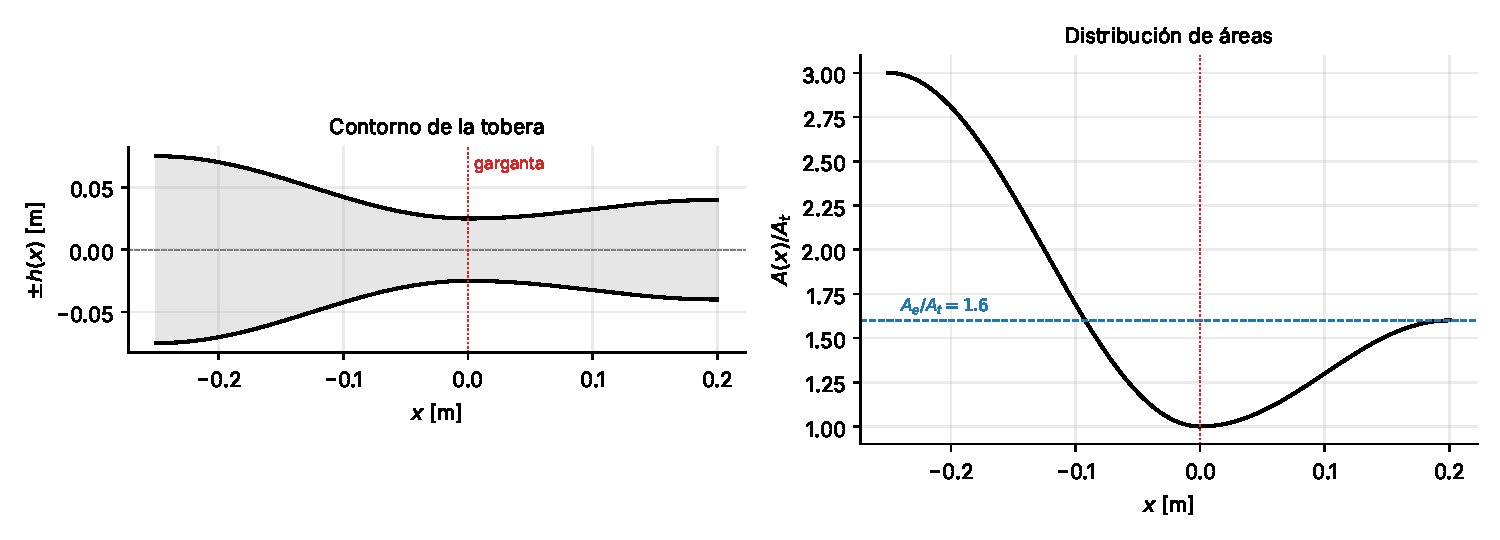
\includegraphics[width=0.95\textwidth]{geometria_Ax.pdf}
     \caption{Contorno de la tobera
     y distribución de áreas $A(x)/A_t$
     obtenidos a partir del perfil cosenoidal.}
     \label{fig:geometria_area_real}
 \end{figure}

\subsection{Relación inversa área--posición}

Para determinar la posición axial
correspondiente a una relación
de áreas conocida dentro del
divergente, se utiliza la
expresión inversa del perfil.

Definiendo:

\begin{equation}
\alpha=\frac{A(x)}{A_t}
\end{equation}

y despejando la coordenada $x$
de la ecuación del divergente,
se obtiene:

\begin{equation}
\boxed{
x(\alpha)=
\frac{L_d}{\pi}
\arccos\left[
1-\frac{2(\alpha-1)}
{A_e/A_t-1}
\right]
}
\label{eq:inversa_area_posicion}
\end{equation}

Esta expresión es válida para:

\begin{equation}
1\leq\alpha\leq1.6
\end{equation}

La función es monótona en
el intervalo divergente,
por lo que cada relación
de áreas corresponde
a una única posición axial.

Esta ecuación se utilizará
posteriormente para determinar
la ubicación teórica del choque
normal en el caso C, una vez
calculada la relación $A_s/A_t$.

\newpage
\section{Metodología y preparación de la simulación}
\label{sec:metodologia}

Esta sección documenta la configuración completa de la simulación: herramientas, dominio, malla, modelo físico, esquemas, condiciones de frontera, control del paso de tiempo y criterio de cierre. Los archivos que reproducen cada paso se describen en el Anexo~\ref{anexo:archivos}.

\subsection{Herramientas y versiones}

\begin{table}[H]
\centering
\caption{Herramientas utilizadas.}
\label{tab:herramientas}
\renewcommand{\arraystretch}{1.2}
\small
\begin{tabular}{p{2.6cm}p{5.2cm}p{6.6cm}}
\toprule
\textbf{Herramienta} & \textbf{Versión} & \textbf{Uso} \\
\midrule
Gmsh & 4.15.2 & Geometría y mallas estructuradas (\texttt{tobera.geo}) \\
OpenFOAM & 8 (blueCFD-Core, Windows, doble precisión) & Solución de las ecuaciones de Euler (\texttt{rhoCentralFoam}) \\
Python 3 & NumPy, SciPy, Matplotlib & Teoría cuasiunidimensional, posproceso, figuras y tablas \\
\bottomrule
\end{tabular}
\end{table}

\subsection{Casos estudiados}

Las condiciones de alimentación son las mismas en los tres casos ($p_{01}=300$ kPa, $T_{01}=300$ K); solo cambia la contrapresión (Tabla~\ref{tab:casos}). Los límites de cada régimen son los de la Tabla~\ref{tab:regimenes_tobera}.

\begin{table}[H]
\centering
\caption{Casos del Nivel 1 y valores teóricos de referencia (semidominio, profundidad $b=0.01$ m).}
\label{tab:casos}
\renewcommand{\arraystretch}{1.2}
\small
\begin{tabular}{llcccc}
\toprule
\textbf{Caso} & \textbf{Régimen} & $p_B$ [kPa] & $p_B/p_{01}$ & \textbf{Mallas} & $\dot m_{teo}$ [kg/s] \\
\midrule
S & Subsónico no estrangulado & 276 & 0.920 & r1, r2 & 0.15642 \\
A & Supersónico adaptado & salida libre & -- & r1, r2 & 0.17502 \\
C & Choque normal interno & 200 & 0.667 & r1, r2, r4 & 0.17502 \\
\bottomrule
\end{tabular}
\end{table}

En el caso A la salida es supersónica y no se impone presión: la presión estática de salida resulta del flujo ($p_e=42.395$ kPa en la teoría). En el caso C, con $p_B=200$ kPa, la posición teórica del choque es $x_s=0.13462$ m ($x_s/L_d=0.6731$), con $M_{s1}=1.8148$, $M_{s2}=0.6132$, $p_2/p_1=3.6757$ y $p_{02}/p_{01}=0.8061$.

El caso S se definió con $p_B=276$ kPa y no con 290 kPa. Con 290 kPa el número de Mach de salida teórico es $M_e=0.22$, un régimen de muy bajo Mach en el que la solución es muy sensible a la pérdida numérica de presión total (Sección~\ref{sec:sens-dt}). Con 276 kPa se tiene $M_t=0.669$ y $M_e=0.347$, y el flujo sigue siendo subsónico sin estrangular (el gasto es 89.4~\% del gasto bloqueado).

\subsection{Dominio y malla}

El dominio es el semidominio superior de la tobera (Sección~\ref{sec:geometria_diseno}), con una sola celda en $z$ ($b=0.01$ m). Las mallas son estructuradas, de celdas hexaédricas con distribución uniforme en $x$ y en $y$ (sin refinamiento local), generadas con el archivo paramétrico \texttt{tobera.geo}. Un factor entero $r$ controla la resolución: el convergente tiene $50r$ celdas en $x$, el divergente $80r$ y todo el dominio $20r$ celdas en $y$. El tamaño de celda en el divergente es $\Delta x=L_d/(80r)$.

\begin{table}[H]
\centering
\caption{Mallas empleadas y calidad según \texttt{checkMesh} (OpenFOAM-8). Todas resultaron \texttt{Mesh OK}.}
\label{tab:mallas}
\renewcommand{\arraystretch}{1.2}
\small\setlength{\tabcolsep}{4pt}
\begin{tabular}{lcccccc}
\toprule
\textbf{Malla} & $r$ & \textbf{Celdas} & $\Delta x$ div. [mm] & \shortstack{Rel. de aspecto\\máx.} & \shortstack{No ortogonalidad\\máx. / media [$^\circ$]} & \shortstack{Asimetría\\máx.} \\
\midrule
r1 & 1 & 2\,600  & 2.50  & 3.996 & 17.2 / 5.11 & 0.152 \\
r2 & 2 & 10\,400 & 1.25  & 3.999 & 17.4 / 5.12 & 0.154 \\
r4 & 4 & 41\,600 & 0.625 & 3.999 & 17.5 / 5.13 & 0.155 \\
\bottomrule
\end{tabular}
\end{table}

Las métricas de la Tabla~\ref{tab:mallas} casi no cambian al refinar porque las tres mallas son refinamientos uniformes de la misma topología. La no ortogonalidad máxima (alrededor de $17^\circ$) se presenta en el convergente, donde la pared tiene la mayor pendiente; en las tres mallas el volumen mínimo de celda es positivo y \texttt{checkMesh} no reporta celdas ni caras problemáticas. Los grupos físicos son \texttt{inlet}, \texttt{outlet}, \texttt{wall}, \texttt{symmetry} y \texttt{frontAndBack}. La Figura~\ref{fig:geometria-mallas} muestra la geometría y el detalle de las tres mallas en la garganta.

\begin{figure}[H]
  \centering
  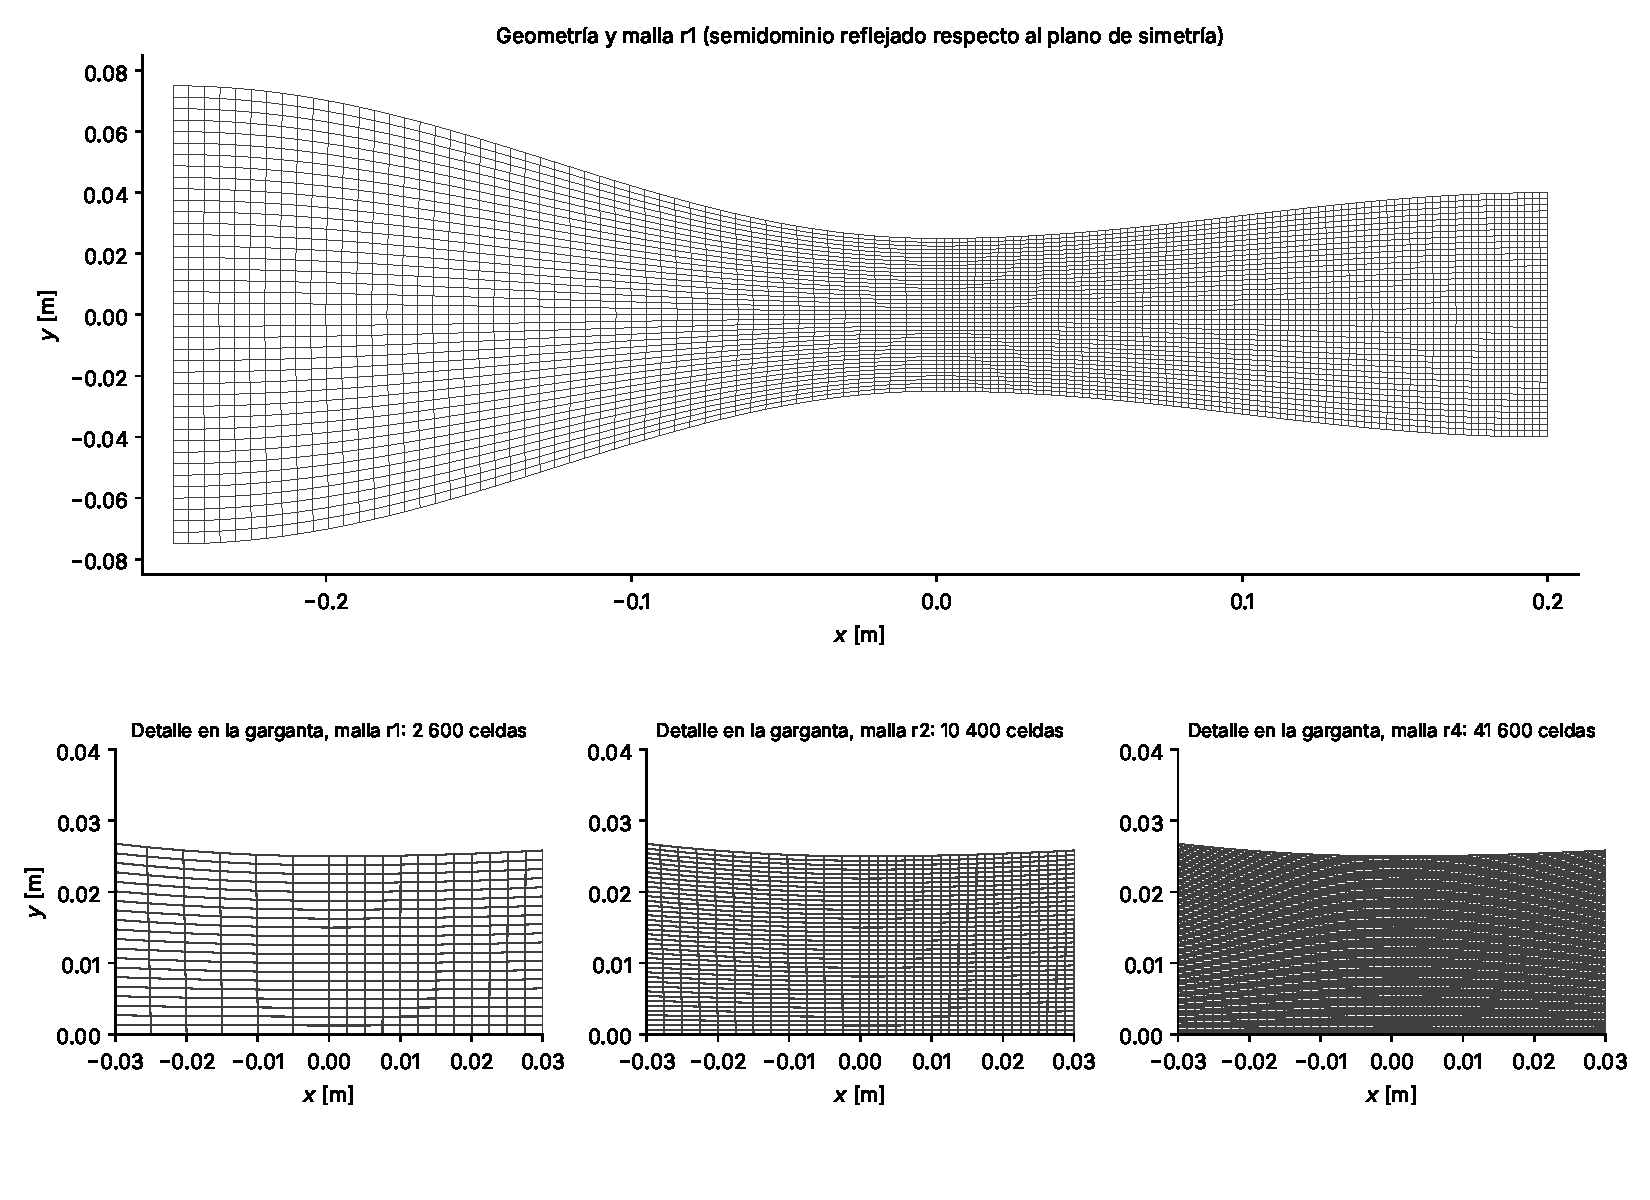
\includegraphics[width=\textwidth]{figuras/geometria_mallas.pdf}
  \caption{Geometría de la tobera y mallas estructuradas utilizadas. Arriba, malla r1 del semidominio reflejado respecto al plano de simetría. Abajo, detalle en la garganta para las mallas r1 (2\,600 celdas), r2 (10\,400) y r4 (41\,600).}
  \label{fig:geometria-mallas}
\end{figure}

\subsection{Modelo físico y propiedades}

Se resuelven las ecuaciones de Euler (Sección~\ref{sec:marco}) para aire como gas perfecto: tipo de termofísica \texttt{hePsiThermo} con \texttt{perfectGas}, \texttt{hConst} y energía interna sensible; masa molar $28.96$ g/mol, $c_p=1004.5$ J/(kg\,K) ($\gamma=1.4$, $R\approx287$ J/(kg\,K)). El flujo es inviscido y adiabático: viscosidad $\mu=0$, $\mathrm{Pr}=1$ y \texttt{simulationType laminar} (que no activa términos viscosos al ser $\mu=0$). Las paredes son deslizantes (\texttt{slip}).

\subsection{Solver y esquemas numéricos}

\begin{table}[H]
\centering
\caption{Esquemas numéricos (archivos \texttt{fvSchemes}, \texttt{fvSolution} y \texttt{controlDict}).}
\label{tab:esquemas}
\renewcommand{\arraystretch}{1.2}
\small
\begin{tabular}{ll}
\toprule
\textbf{Elemento} & \textbf{Configuración} \\
\midrule
Solver & \texttt{rhoCentralFoam} (en serie) \\
Flujo numérico & Kurganov \\
Reconstrucción de $\rho$, $\mathbf U$, $T$ & \texttt{vanLeer}, \texttt{vanLeerV}, \texttt{vanLeer} \\
Integración en el tiempo & Euler explícita, paso adaptativo \\
Gradientes & \texttt{Gauss linear} \\
Courant máximo (casos de referencia) & 0.1 \\
Paso máximo & $10^{-5}$ s \\
Escritura de resultados & cada 0.001 s \\
\bottomrule
\end{tabular}
\end{table}

\subsection{Condiciones iniciales y de frontera}

\begin{table}[H]
\centering
\caption{Condiciones de frontera.}
\label{tab:fronteras}
\renewcommand{\arraystretch}{1.2}
\small
\begin{tabular}{p{2.5cm}p{3.9cm}p{4.1cm}p{4.3cm}}
\toprule
\textbf{Frontera} & $p$ & $T$ & $\mathbf U$ \\
\midrule
\texttt{inlet} & \texttt{total\-Pressure} ($p_0=300$ kPa) & \texttt{total\-Temperature} ($T_0=300$ K) & \texttt{pressure\-Inlet\-Outlet\-Velocity} \\
\texttt{outlet} (S y C) & \texttt{fixedValue} ($p_B$) & \texttt{zeroGradient} & \texttt{inletOutlet} \\
\texttt{outlet} (A) & \texttt{zeroGradient} & \texttt{zeroGradient} & \texttt{inletOutlet} \\
\texttt{wall} & \texttt{zeroGradient} & \texttt{zeroGradient} & \texttt{slip} \\
\texttt{symmetry} & \texttt{symmetryPlane} & \texttt{symmetryPlane} & \texttt{symmetryPlane} \\
\texttt{frontAndBack} & \texttt{empty} & \texttt{empty} & \texttt{empty} \\
\bottomrule
\end{tabular}
\end{table}

Como condición inicial, el caso A parte de $p=101\,325$ Pa, $T=300$ K y velocidad nula, y el caso C de $p=p_B$ uniforme con $T=300$ K y velocidad nula. Los casos S de referencia se inicializaron con un campo no uniforme preexistente, el mismo en todas las corridas S, para acortar el transitorio; una corrida con campo inicial uniforme dio el mismo resultado final dentro de 0.04 puntos porcentuales (Sección~\ref{sec:sens-dt}) y la estacionariedad se comprobó con el criterio de la Sección~\ref{sec:criterio}.

\subsection{Procesamiento de resultados}
\label{sec:criterio}

El flujo con choques y la disipación numérica impiden que los residuos lleguen a cero, por lo que la convergencia se evalúa con observables físicos promediados en ventanas de tiempo. Para cada caso:

\begin{enumerate}
  \item Se promedian en el tiempo los campos dentro de una ventana (Tabla~\ref{tab:errores-perfiles}) y, en cada sección transversal, se promedian $p$, $T$ y $U_x$ sobre la altura. Esta es la comparación consistente con un modelo cuasiunidimensional; la comparación en una sola celda sobre el eje introduce un sesgo, porque el flujo bidimensional no es exactamente uniforme en la sección.
  \item El número de Mach de sección se calcula como $M=U_x/\sqrt{\gamma R T}$ con los promedios de sección. Es el Mach de la velocidad y la temperatura promediadas por sección, no el promedio de los valores locales de Mach. Con el campo final de las mallas de referencia se comprobó que ambas definiciones difieren, en promedio sobre las secciones, entre 0.36 y 0.46~\% (mediana cercana a 0.19~\%), con máximos locales de 1.5 a 3.7~\% en puntos aislados; esa diferencia es del mismo orden que los errores medios de $M$ reportados (0.1 a 0.3~\%), por lo que éstos deben leerse como errores de la magnitud definida así, la misma en todas las tablas y figuras.
  \item El error relativo en cada sección es $\varepsilon=|\,\phi_{CFD}-\phi_{teo}\,|/\phi_{teo}$. Se reportan el error medio y el RMS sobre todas las secciones; en el caso C se excluye una franja de $\pm 0.03$ m alrededor del choque.
  \item El gasto másico es el flujo por la frontera \texttt{inlet} y por la frontera \texttt{outlet} (suma de $\phi$ por cara, donde $\phi$ es el flujo másico $\rho\,\mathbf{U}\cdot\mathbf{S}_f$ en kg/s de la formulación compresible de \texttt{rhoCentralFoam}; es negativo en la entrada, por lo que se usa su valor absoluto y el semidominio de espesor 0.01~m), y su error es $|\dot m_{CFD}-\dot m_{teo}|/\dot m_{teo}$. El balance de masa es $|\dot m_{ent}-\dot m_{sal}|/\dot m_{ent}$.
  \item La posición del choque $x_s$ es el cruce interpolado de $M=1$ aguas abajo del choque en el perfil de $M$ de sección. Los estados antes y después se miden a tres celdas de distancia ($x_s\mp3\Delta x$), fuera del espesor numérico del choque, y se comparan con la teoría evaluada en las mismas posiciones.
\end{enumerate}

Se considera que el caso convergió cuando (i) los promedios de ventanas consecutivas cambian menos de 1~\%, (ii) el gasto de entrada y el de salida coinciden dentro de 1~\%, y (iii) en el caso C la posición del choque cambia menos de 0.5~\% de $L_d$ entre ventanas.

\newpage
\section{Resultados y discusión}
\label{sec:resultados}

Todos los resultados de esta sección corresponden a las corridas de referencia (Courant máximo 0.1; Tabla~\ref{tab:corridas-completa}). Para cada caso se presenta la verificación (estacionariedad y balance de masa), la comparación con la teoría cuasiunidimensional con el área real $A(x)$, los errores y su discusión. Las magnitudes teóricas son las de la Sección~\ref{sec:metodologia}.

\subsection{Verificación: estacionariedad y balance de masa}

La Figura~\ref{fig:gasto-historias} muestra la historia del gasto másico de entrada y de salida de un caso representativo de cada régimen (A, S y C en la malla r2); las historias de las demás corridas están en los archivos \texttt{gastoEntrada\_*.csv} y \texttt{gastoSalida\_*.csv} del paquete de entrega y siguen el mismo comportamiento. Tras el transitorio inicial (ondas acústicas que cruzan el dominio y se reflejan) ambos gastos se estabilizan y coinciden. La Figura~\ref{fig:conv-ventanas} muestra el criterio de convergencia por ventanas de 10 ms: en el caso C la posición del choque cambia menos de 0.05~\% de $L_d$ entre ventanas, y el error del gasto de salida deja de cambiar después de la primera ventana. El balance de masa entre entrada y salida cierra dentro de 0.005~\% en todos los casos (Tabla~\ref{tab:errores-gasto}), con lo que se cumplen los tres criterios de la Sección~\ref{sec:criterio}.

\begin{figure}[H]
  \centering
  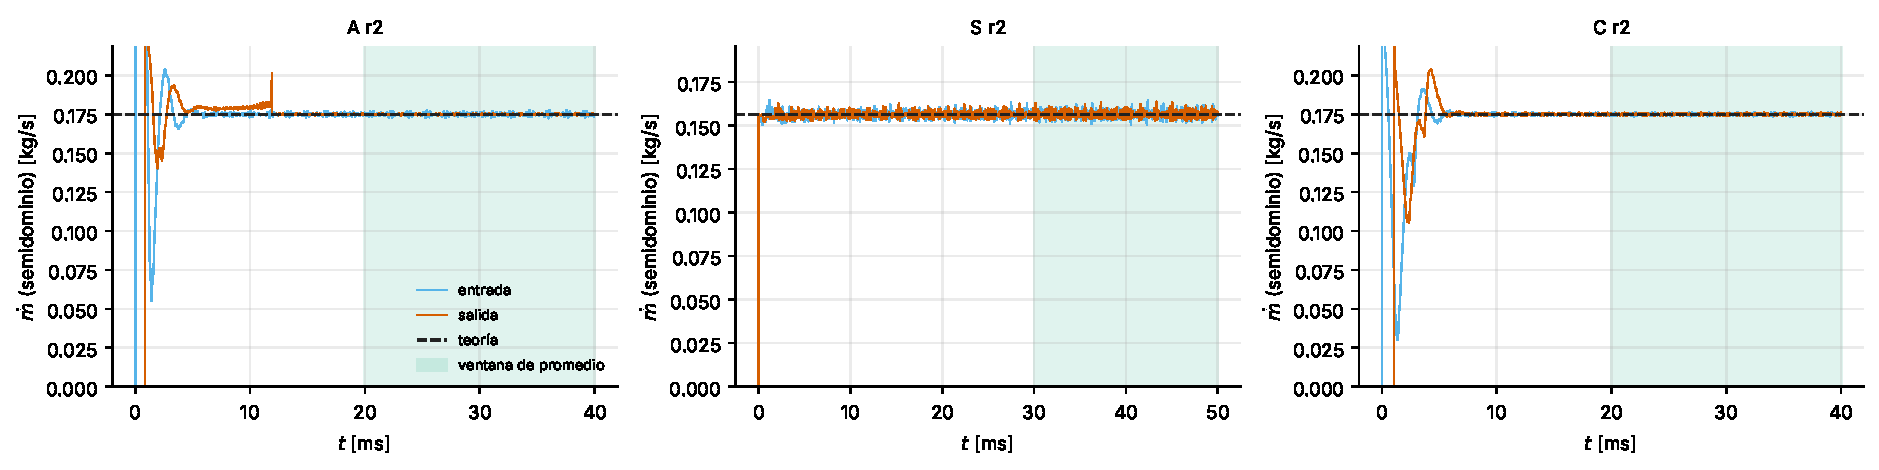
\includegraphics[width=\textwidth]{figuras/gasto_historias.pdf}
  \caption{Historias del gasto másico de entrada y de salida en los casos A, S y C (malla r2), como muestra representativa de cada régimen. El balance de masa cierra dentro de los criterios de convergencia una vez superado el transitorio inicial.}
  \label{fig:gasto-historias}
\end{figure}

\begin{figure}[H]
  \centering
  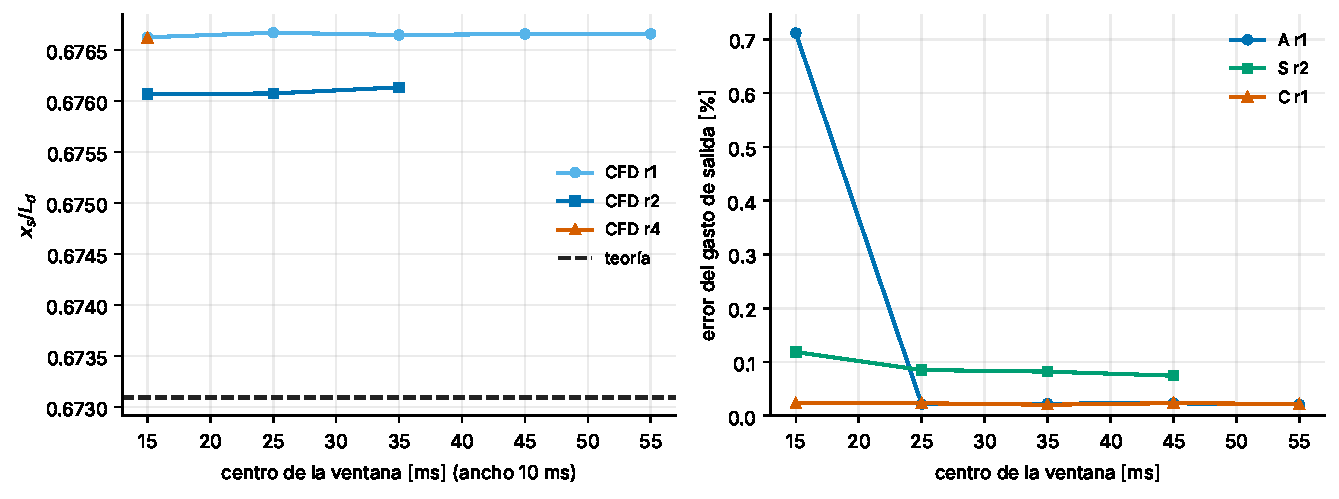
\includegraphics[width=\textwidth]{figuras/convergencia_ventanas.pdf}
  \caption{Convergencia por ventanas de tiempo de 10 ms. Izquierda: posición adimensional del choque en el caso C para las tres mallas. Derecha: error del gasto de salida para los casos A, S y C. Ambas magnitudes presentan variaciones entre ventanas consecutivas inferiores a los criterios establecidos en la Sección~\ref{sec:criterio}.}
  \label{fig:conv-ventanas}
\end{figure}

La Tabla~\ref{tab:ventanas-eq} comprueba el criterio (i) con dos ventanas consecutivas de 5~ms al final de cada corrida, la misma longitud para todos los casos y mallas (incluida r4). El cambio medio del Mach de sección entre ventanas es menor que 0.4~\%, y el máximo local menor que 1~\% en todos los casos (el mayor, 0.96~\%, en S r2). El gasto de salida cambia menos de 0.05~\%, el balance de masa en esas ventanas es menor que 0.05~\% (en las ventanas de promedio de las tablas de resultados, menor que 0.005~\%) y la posición del choque cambia menos de 0.01~\% de $L_d$. En r4 solo se pueden formar ventanas de 5~ms con datos ya estacionarios, porque la corrida llega a 20~ms; por eso su promedio abarca 8~ms (0.012 a 0.020~s) frente a 20 a 60~ms en las otras mallas.

\begin{table}[H]
\centering
\caption{Cambio entre dos ventanas consecutivas de 5~ms al final de cada corrida (Courant 0.1).}
\label{tab:ventanas-eq}
\small
\renewcommand{\arraystretch}{1.15}
\begin{tabular}{lcccccc}
\toprule
Caso & Ventanas [ms] & $\Delta M$ medio [\%] & $\Delta M$ máx. [\%] & $\Delta\dot m_{sal}$ [\%] & Balance [\%] & $\Delta x_s/L_d$ [\%] \\
\midrule
A r1 & 50--55--60 & 0.024 & 0.12 & 0.001 & 0.002 & -- \\
A r2 & 30--35--40 & 0.086 & 0.52 & 0.001 & 0.008 & -- \\
S r1 & 90--95--100 & 0.060 & 0.21 & 0.026 & 0.016 & -- \\
S r2 & 40--45--50 & 0.375 & 0.96 & 0.043 & 0.049 & -- \\
C r1 & 50--55--60 & 0.027 & 0.15 & 0.005 & 0.001 & 0.001 \\
C r2 & 30--35--40 & 0.095 & 0.52 & 0.006 & 0.006 & 0.002 \\
C r4 & 10--15--20 & 0.086 & 0.38 & 0.001 & 0.004 & 0.003 \\
\bottomrule
\end{tabular}
\end{table}

El caso S es el que más tarda en alcanzar el estado estacionario, porque en flujo subsónico las perturbaciones acústicas se propagan en ambos sentidos y se amortiguan lentamente; por eso su ventana de promedio es más tardía (0.04--0.10~s en r1).

\begin{table}[H]
\centering
\caption{Errores medios de los perfiles CFD respecto a la teoría cuasiunidimensional (promedio en la ventana de tiempo indicada; en el caso C se excluye $\pm0.03$ m alrededor del choque).}
\label{tab:errores-perfiles}
\footnotesize\setlength{\tabcolsep}{3pt}
\begin{tabular}{llcrrrr}
\toprule
Caso & Malla & Ventana [s] & Error $M$ medio [\%] & RMS $M$ [\%] & Error $p/p_{01}$ medio [\%] & Error $T/T_{01}$ medio [\%] \\
\midrule
A & r1 & 0.03--0.06 & 0.22 & 0.26 & 0.27 & 0.07 \\
A & r2 & 0.02--0.04 & 0.22 & 0.27 & 0.27 & 0.07 \\
S & r1 & 0.04--0.1 & 0.08 & 0.10 & 0.07 & 0.03 \\
S & r2 & 0.03--0.05 & 0.09 & 0.12 & 0.08 & 0.03 \\
C & r1 & 0.03--0.06 & 0.20 & 0.25 & 0.23 & 0.06 \\
C & r2 & 0.02--0.04 & 0.22 & 0.27 & 0.23 & 0.06 \\
C & r4 & 0.012--0.02 & 0.21 & 0.27 & 0.25 & 0.07 \\
\bottomrule
\end{tabular}
\end{table}

\begin{table}[H]
\centering
\caption{Gasto másico del semidominio: CFD frente a teoría y balance de masa entre entrada y salida.}
\label{tab:errores-gasto}
\footnotesize\setlength{\tabcolsep}{3pt}
\begin{tabular}{llrrrr}
\toprule
Caso & Malla & $\dot m$ CFD [kg/s] & $\dot m$ teoría [kg/s] & Error $\dot m$ [\%] & Balance de masa [\%] \\
\midrule
A & r1 & 0.17498 & 0.17502 & 0.022 & 0.000 \\
A & r2 & 0.17497 & 0.17502 & 0.025 & 0.003 \\
S & r1 & 0.15627 & 0.15642 & 0.097 & 0.000 \\
S & r2 & 0.15629 & 0.15642 & 0.078 & 0.005 \\
C & r1 & 0.17498 & 0.17502 & 0.022 & 0.000 \\
C & r2 & 0.17497 & 0.17502 & 0.025 & 0.002 \\
C & r4 & 0.17495 & 0.17502 & 0.040 & 0.001 \\
\bottomrule
\end{tabular}
\end{table}


\subsection{Caso S: subsónico no estrangulado}

La Figura~\ref{fig:perfiles-S} compara los perfiles de $M$, $p/p_{01}$ y $T/T_{01}$ con la teoría (malla r2), y la Figura~\ref{fig:mapas-S} muestra los campos. El flujo se acelera en el convergente hasta $M_t\approx0.67$ en la garganta y se desacelera en el divergente, sin alcanzar la condición sónica.

\begin{figure}[H]
  \centering
  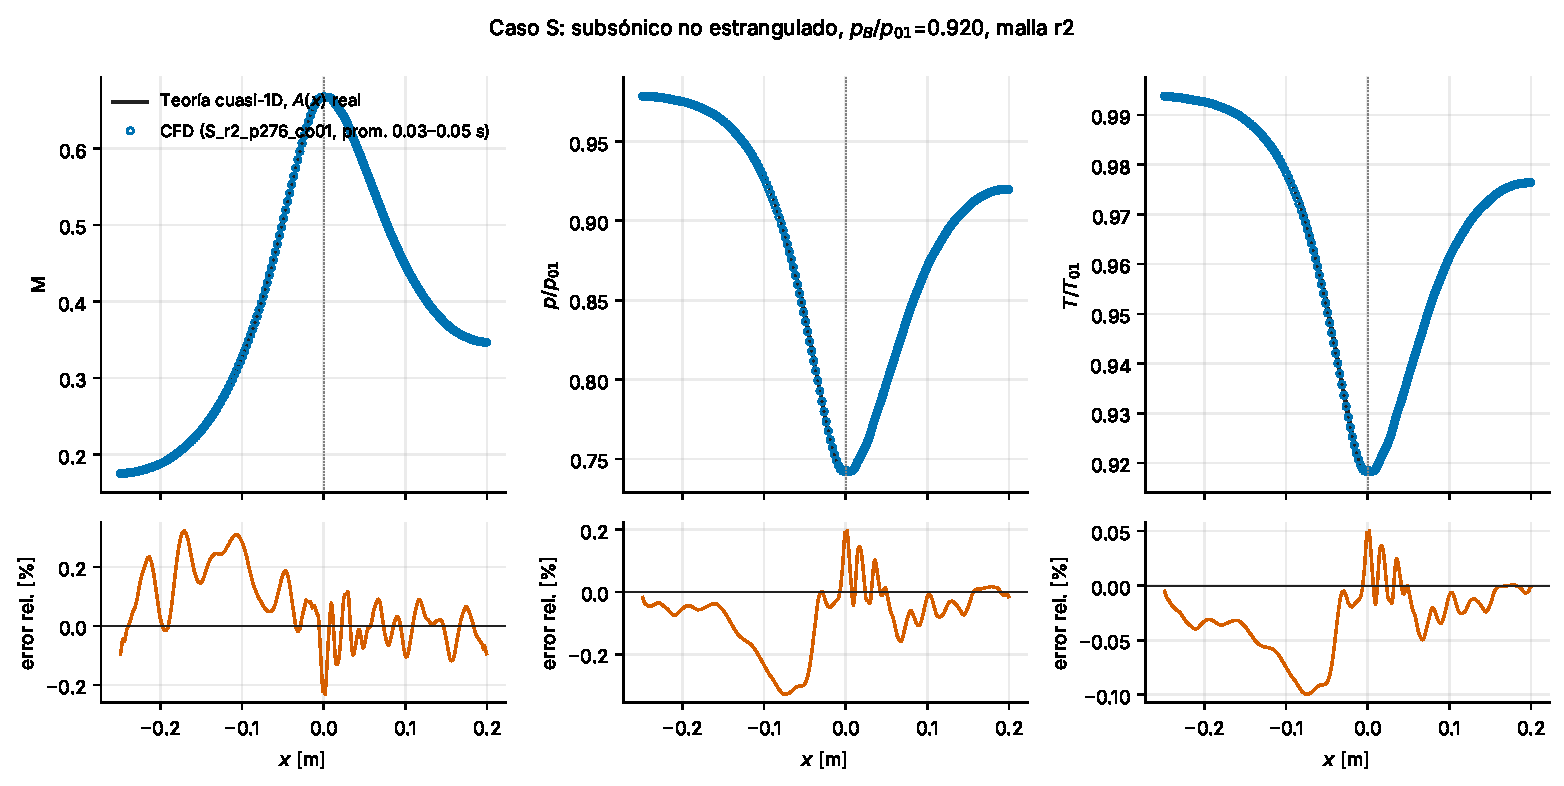
\includegraphics[width=0.85\textwidth]{figuras/perfiles_S_r2.pdf}
  \caption{Caso S (subsónico no estrangulado, $p_B=276$ kPa), malla r2. Perfiles de Mach, presión y temperatura a lo largo de la tobera, promediados por sección transversal y en una ventana de tiempo, contra la solución cuasiunidimensional con la distribución real $A(x)$.}
  \label{fig:perfiles-S}
\end{figure}

\begin{figure}[H]
  \centering
  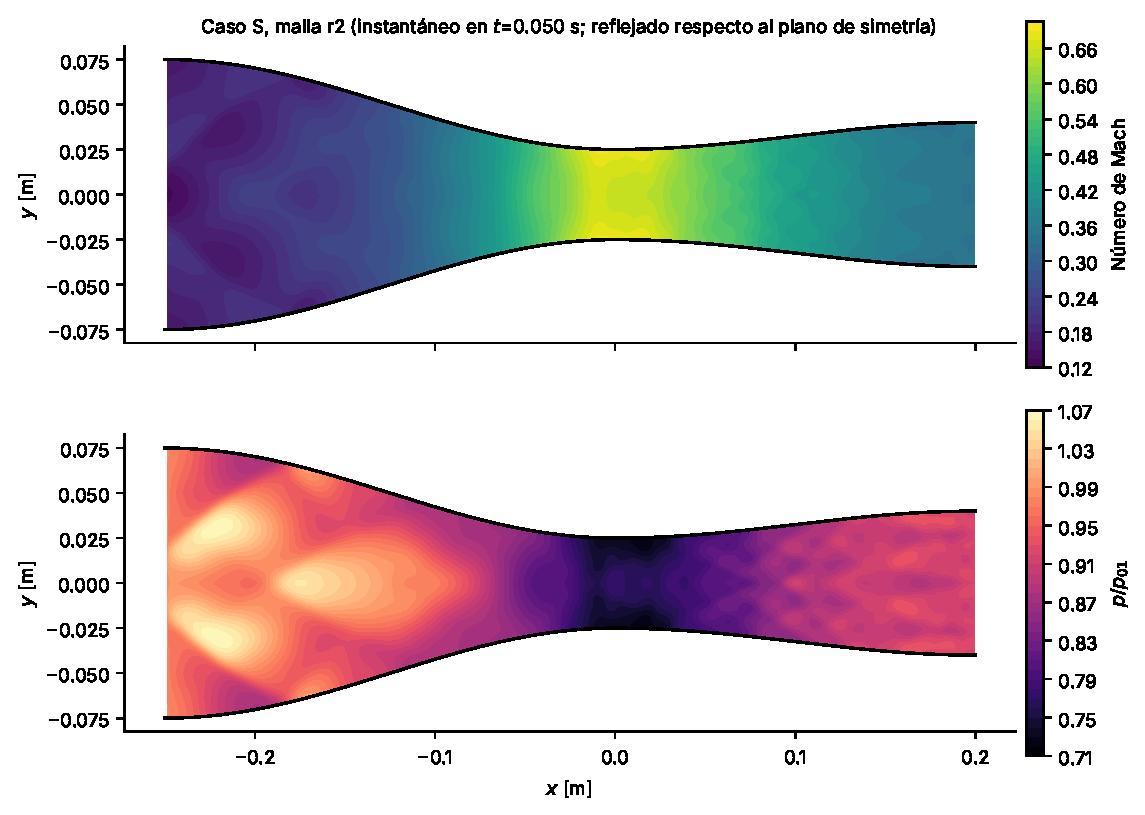
\includegraphics[width=0.8\textwidth]{figuras/mapas_S_r2.pdf}
  \caption{Caso S, malla r2: campos de número de Mach y de presión adimensional $p/p_{01}$ (semidominio reflejado).}
  \label{fig:mapas-S}
\end{figure}

El error medio del número de Mach es de 0.08~\% (r1) y 0.09~\% (r2), el de la presión de 0.07 y 0.08~\%, y el del gasto de 0.097 y 0.078~\% (Tablas~\ref{tab:errores-perfiles} y~\ref{tab:errores-gasto}). En la sección de salida (Tablas~\ref{tab:estado-salida} y~\ref{tab:estado-salida-err}), $M_e=0.3469$ frente a 0.3472 teórico y $p_e=275.9$ kPa frente a 276.0 kPa; la velocidad de salida es $V_e=119.0$ m/s ($119.1$ m/s en la teoría). Estas diferencias son menores que 0.1~\%, lo que confirma que el modelo reproduce la solución isentrópica cuasiunidimensional cuando el paso de tiempo es suficientemente pequeño.

\subsection{Caso A: supersónico adaptado}

\begin{figure}[H]
  \centering
  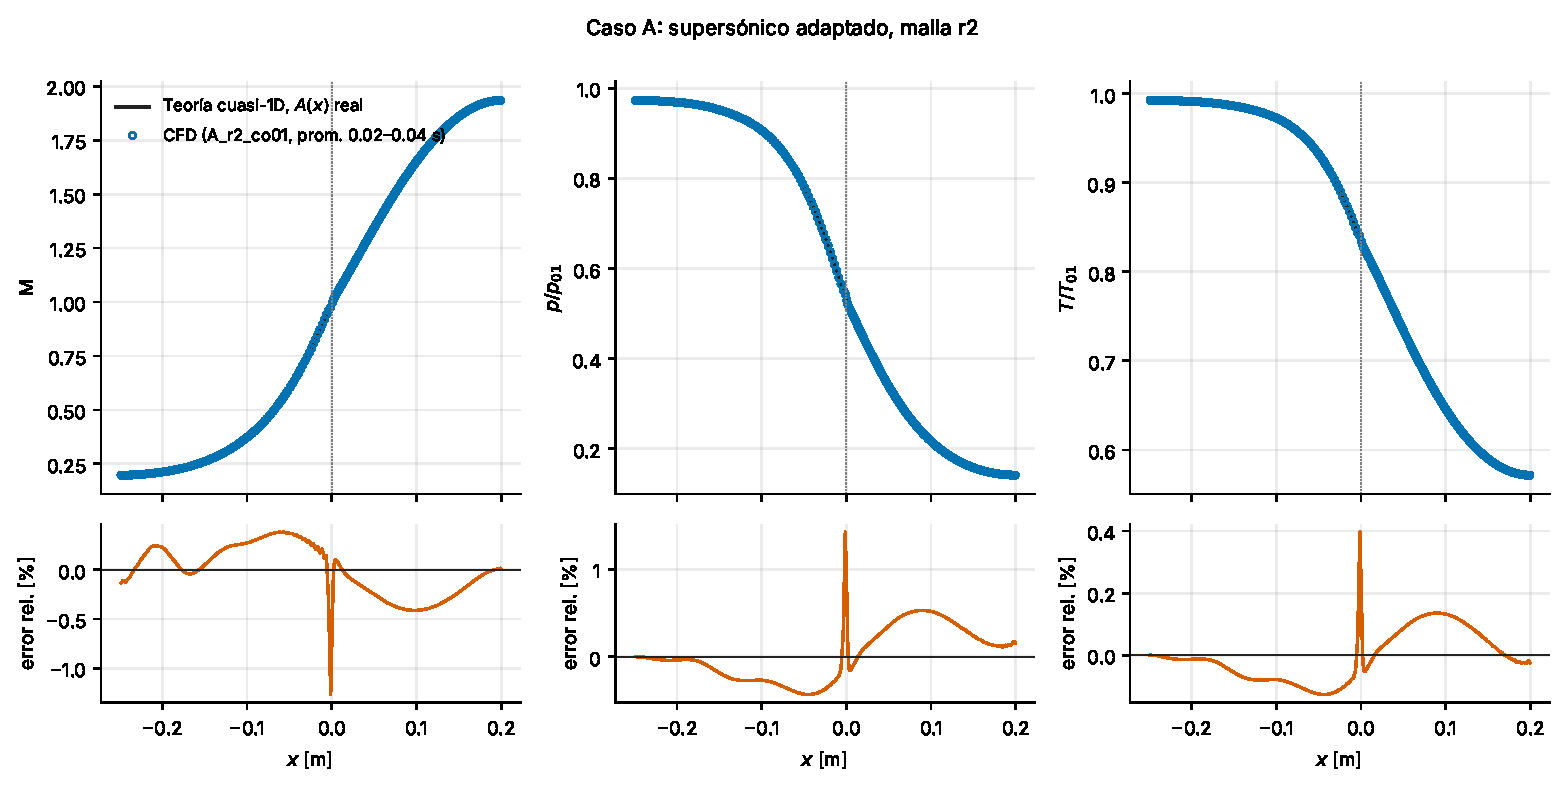
\includegraphics[width=0.85\textwidth]{figuras/perfiles_A_r2.pdf}
  \caption{Caso A (supersónico adaptado), malla r2. Perfiles CFD (promedio por sección transversal y en ventana de tiempo) frente a la teoría cuasiunidimensional (rama supersónica).}
  \label{fig:perfiles-A}
\end{figure}

\begin{figure}[H]
  \centering
  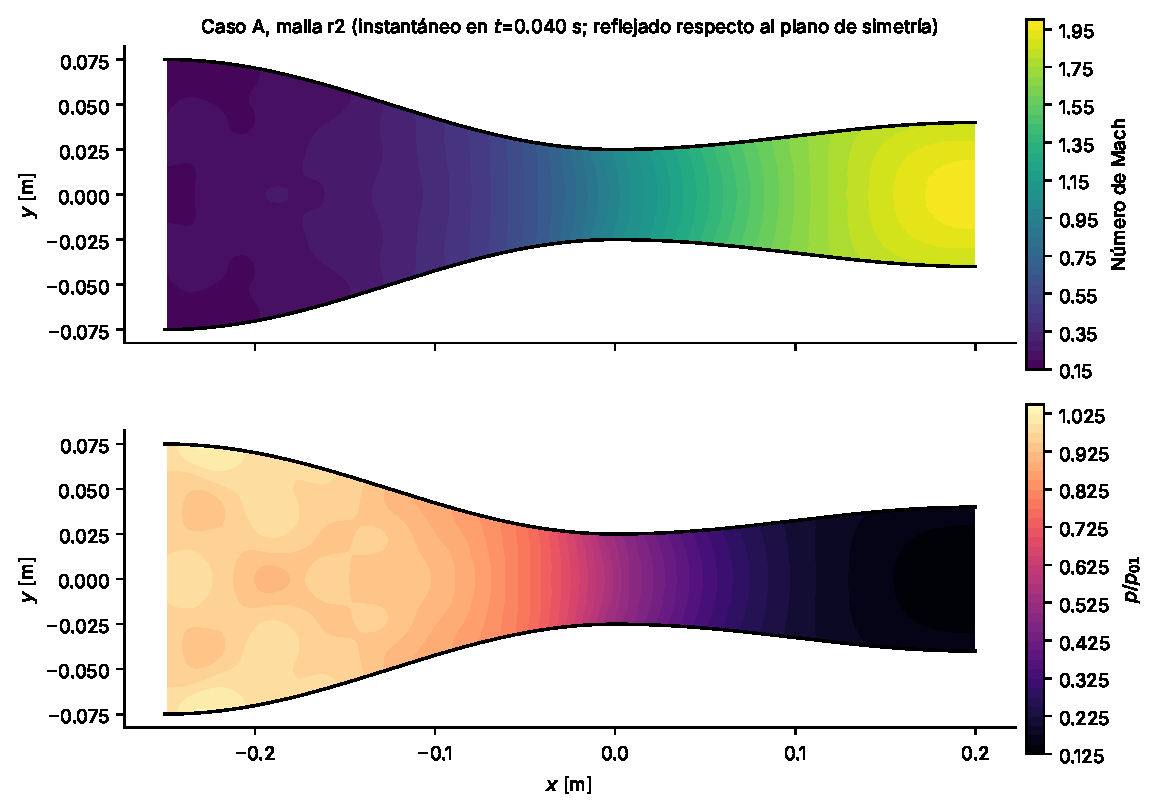
\includegraphics[width=0.8\textwidth]{figuras/mapas_A_r2.pdf}
  \caption{Caso A, malla r2: campos de número de Mach y de presión adimensional $p/p_{01}$.}
  \label{fig:mapas-A}
\end{figure}

El flujo alcanza $M=1$ en la garganta y se acelera hasta $M_e=1.9355$ en la salida (teoría: 1.9353). La presión de salida es de 42.46 kPa frente a 42.40 kPa (error de 0.16~\%); el error mayor de las magnitudes de salida es el de la presión (Tablas~\ref{tab:estado-salida} y~\ref{tab:estado-salida-err}). El error medio del Mach a lo largo de la tobera es 0.22~\% con ambas mallas y el del gasto es 0.022~\% (r1) y 0.025~\% (r2). El gasto de 0.17498 kg/s (semidominio) coincide con el gasto bloqueado teórico de 0.17502 kg/s, lo que indica que la garganta está estrangulada. Los resultados de r1 y r2 son prácticamente idénticos, lo que indica baja sensibilidad a la malla en este régimen, aunque con solo dos mallas no se demuestra independencia rigurosa.

\begin{table}[H]
\centering
\caption{Estado en la sección de salida: CFD (promedio de sección y de ventana) contra teoría cuasiunidimensional.}
\label{tab:estado-salida}
\footnotesize\setlength{\tabcolsep}{3pt}
\begin{tabular}{llrrrrrrrr}
\toprule
Caso & Malla & $M_e$ CFD & $M_e$ teo. & $p_e$ CFD [kPa] & $p_e$ teo. [kPa] & $T_e$ CFD [K] & $T_e$ teo. [K] & $V_e$ CFD [m/s] & $V_e$ teo. [m/s] \\
\midrule
A & r1 & 1.9354 & 1.9352 & 42.47 & 42.40 & 171.49 & 171.53 & 508.0 & 508.0 \\
A & r2 & 1.9355 & 1.9352 & 42.46 & 42.40 & 171.48 & 171.52 & 508.0 & 508.0 \\
S & r1 & 0.3469 & 0.3472 & 275.92 & 276.00 & 292.94 & 292.94 & 119.0 & 119.1 \\
S & r2 & 0.3469 & 0.3472 & 275.96 & 276.00 & 292.93 & 292.94 & 119.0 & 119.1 \\
C & r1 & 0.5282 & 0.5280 & 199.97 & 200.00 & 284.16 & 284.15 & 178.5 & 178.4 \\
C & r2 & 0.5280 & 0.5280 & 200.00 & 200.00 & 284.16 & 284.16 & 178.4 & 178.4 \\
C & r4 & 0.5286 & 0.5280 & 199.96 & 200.00 & 284.12 & 284.16 & 178.6 & 178.4 \\
\bottomrule
\end{tabular}
\end{table}

\begin{table}[H]
\centering
\caption{Errores relativos en la sección de salida.}
\label{tab:estado-salida-err}
\small\setlength{\tabcolsep}{4pt}
\begin{tabular}{llrrrr}
\toprule
Caso & Malla & Error $M_e$ [\%] & Error $p_e$ [\%] & Error $T_e$ [\%] & Error $V_e$ [\%] \\
\midrule
A & r1 & 0.01 & 0.17 & 0.02 & 0.00 \\
A & r2 & 0.01 & 0.16 & 0.02 & 0.00 \\
S & r1 & 0.08 & 0.03 & 0.00 & 0.08 \\
S & r2 & 0.09 & 0.01 & 0.00 & 0.09 \\
C & r1 & 0.03 & 0.01 & 0.00 & 0.03 \\
C & r2 & 0.01 & 0.00 & 0.00 & 0.01 \\
C & r4 & 0.10 & 0.02 & 0.01 & 0.10 \\
\bottomrule
\end{tabular}
\end{table}


\subsection{Caso C: choque normal interno}

\begin{figure}[H]
  \centering
  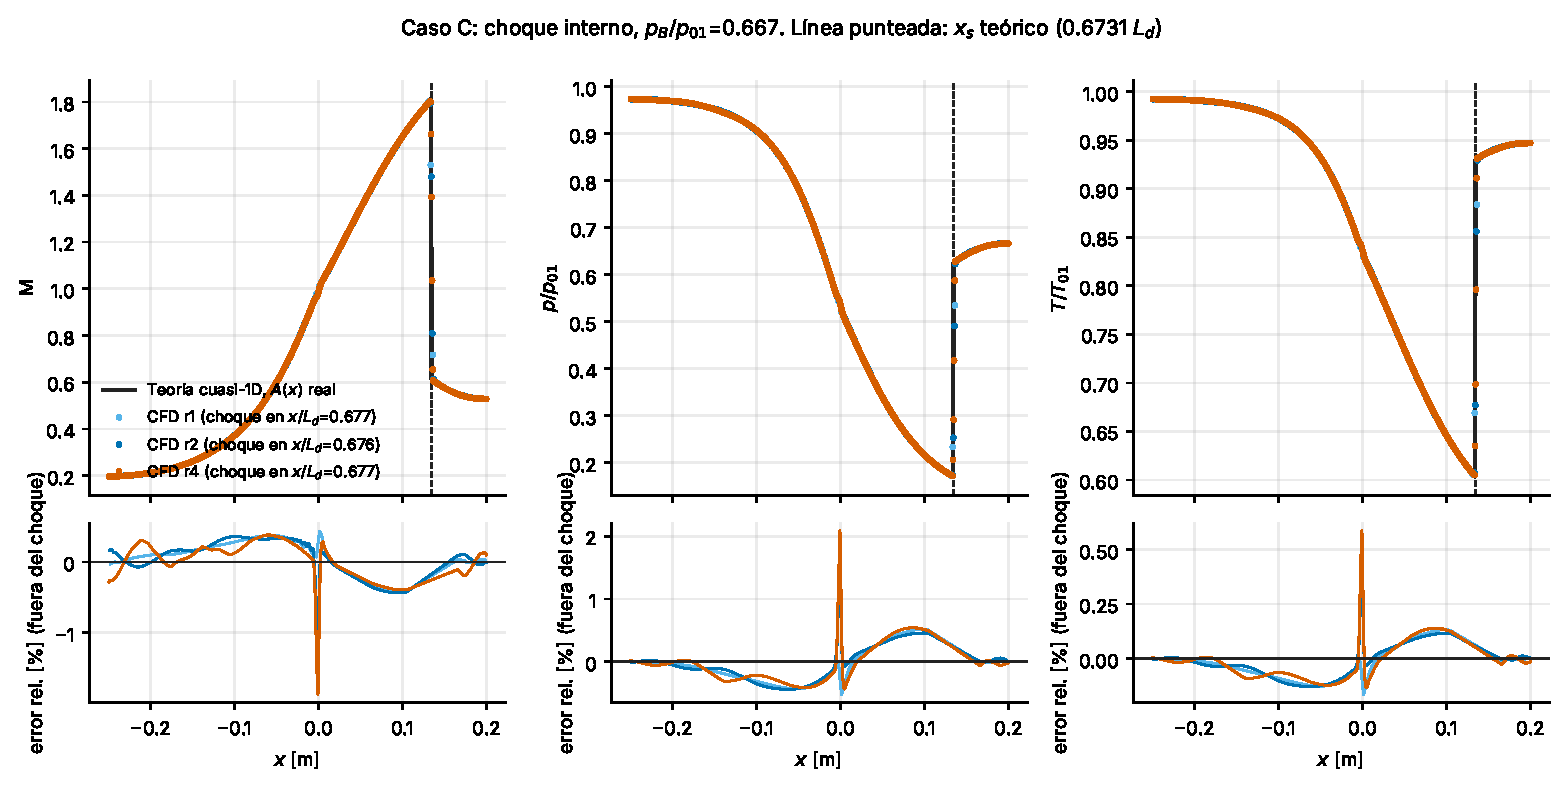
\includegraphics[width=0.85\textwidth]{figuras/perfiles_C_mallas.pdf}
  \caption{Caso C (choque interno, $p_B=200$ kPa). Perfiles (promedio por sección transversal y en ventana de tiempo) obtenidos con las mallas r1, r2 y r4 frente a la teoría; el choque se ubica en $x_s/L_d\approx0.676$ en las tres mallas (teoría: 0.673).}
  \label{fig:perfiles-C}
\end{figure}

\begin{figure}[H]
  \centering
  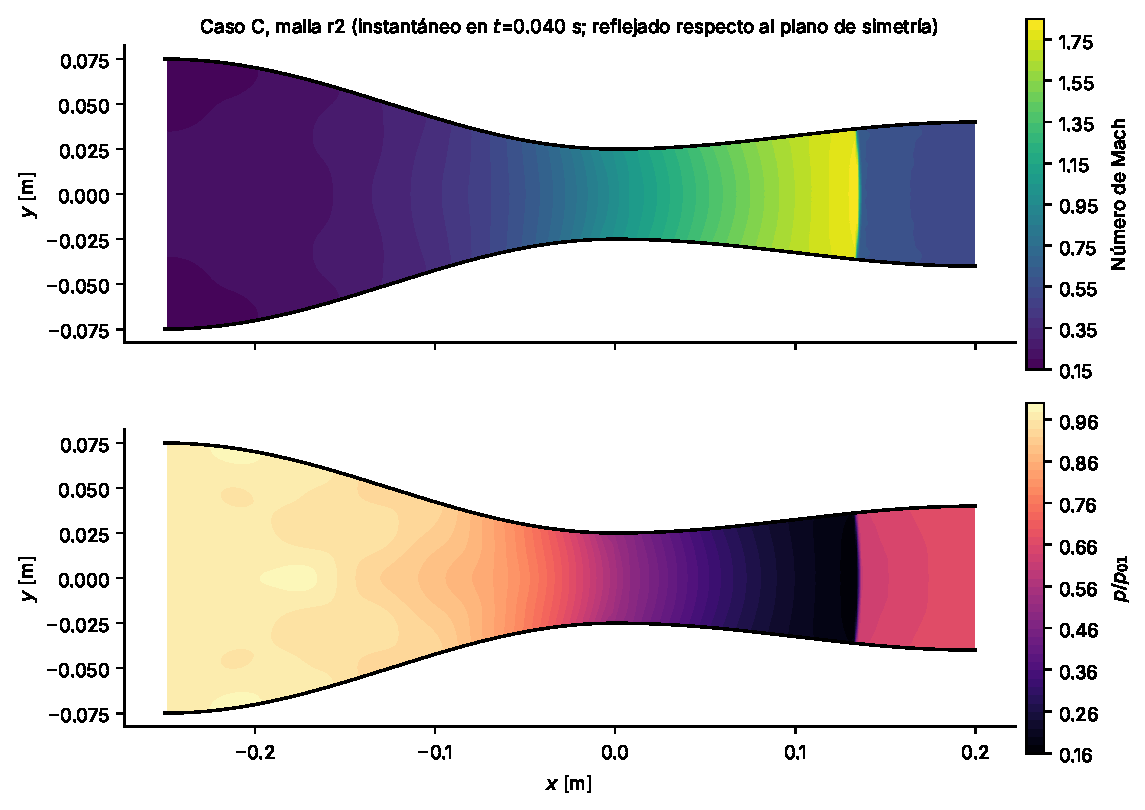
\includegraphics[width=0.8\textwidth]{figuras/mapas_C_r2.pdf}
  \caption{Caso C, malla r2: campos de número de Mach y de presión adimensional $p/p_{01}$. Se aprecia el choque normal en el divergente y el flujo subsónico aguas abajo.}
  \label{fig:mapas-C}
\end{figure}

El flujo se acelera hasta $M\approx1.8$ en el divergente, se produce un choque normal casi plano en $x_s\approx0.135$ m, y el flujo subsónico posterior se desacelera hasta $M_e=0.528$ en la salida (teoría: 0.528). Las Tablas~\ref{tab:choque-C} y~\ref{tab:choque-C-estados} comparan el choque con la teoría. La posición del choque está a 0.30--0.36~\% de $L_d$ de la teórica; $M_{s1}$ y $M_{s2}$ difieren de la teoría en menos de 1~\% (r2: 1.799 contra 1.804 y 0.601 contra 0.600), y la relación de presiones totales $p_{02}/p_{01}$ es 0.810 frente a 0.806 (0.5~\% de diferencia), es decir, la pérdida de presión total por el choque se reproduce. La relación $p_2/p_1$ es de 3.64 contra 3.66 teórico. La ligera curvatura del choque que se observa en la Figura~\ref{fig:mapas-C} es un efecto bidimensional que el modelo cuasiunidimensional no representa.

\begin{table}[H]
\centering
\caption{Choque normal del caso C: posición y área en el choque.}
\label{tab:choque-C}
\footnotesize\setlength{\tabcolsep}{3pt}
\begin{tabular}{lcrrrrrrr}
\toprule
Malla & Ventana [s] & $x_s$ CFD [m] & $x_s$ teo. [m] & $x_s/L_d$ CFD & $x_s/L_d$ teo. & Error pos. [\% $L_d$] & $A_s/A_t$ CFD & $A_s/A_t$ teo. \\
\midrule
r1 & 0.03--0.06 & 0.1353 & 0.1346 & 0.6767 & 0.6731 & 0.36 & 1.4581 & 1.4552 \\
r2 & 0.02--0.04 & 0.1352 & 0.1346 & 0.6761 & 0.6731 & 0.30 & 1.4576 & 1.4552 \\
r4 & 0.012--0.02 & 0.1353 & 0.1346 & 0.6766 & 0.6731 & 0.35 & 1.4580 & 1.4552 \\
\bottomrule
\end{tabular}
\end{table}

\begin{table}[H]
\centering
\caption{Estados antes ($1$, en $x_1=x_s-3\Delta x$) y después ($2$, en $x_2=x_s+3\Delta x$) del choque, medidos fuera de su espesor numérico, contra la teoría evaluada en las mismas posiciones.}
\label{tab:choque-C-estados}
\footnotesize\setlength{\tabcolsep}{3pt}
\begin{tabular}{lrrrrrrrr}
\toprule
Malla & $M_{s1}$ CFD & $M_{s1}$ teo. & $M_{s2}$ CFD & $M_{s2}$ teo. & $p_2/p_1$ CFD & $p_2/p_1$ teo. & $p_{02}/p_{01}$ CFD & $p_{02}/p_{01}$ teo. \\
\midrule
r1 & 1.785 & 1.792 & 0.590 & 0.589 & 3.597 & 3.619 & 0.8100 & 0.8061 \\
r2 & 1.799 & 1.804 & 0.601 & 0.600 & 3.637 & 3.655 & 0.8099 & 0.8061 \\
r4 & 1.801 & 1.810 & 0.605 & 0.606 & 3.642 & 3.671 & 0.8105 & 0.8061 \\
\bottomrule
\end{tabular}
\end{table}


\subsection{Estudio de sensibilidad de malla}

El estudio de malla se hizo en el caso C con las mallas r1, r2 y r4 (Figura~\ref{fig:conv-malla-C}). Los errores son menores que 0.4~\% de $L_d$ en la posición del choque, 0.3~\% en $M$ y $p/p_{01}$ y 0.04~\% en el gasto, y no disminuyen de forma monótona al refinar: la posición del choque pasa de 0.35~\% (r1) a 0.30~\% (r2) y a 0.35~\% (r4), y el error del gasto sube de 0.022~\% a 0.040~\%. Esto indica que la sensibilidad a la malla es pequeña, pero con tres mallas y errores que no decrecen de forma sistemática no se puede demostrar una convergencia rigurosa (no se estimó un orden de convergencia ni un índice de convergencia de malla). El error restante puede deberse tanto a la discretización espacial como a la diferencia entre el modelo bidimensional y el cuasiunidimensional (por ejemplo, la curvatura del choque y la no uniformidad de la sección), y con estos datos no se puede separar la contribución de cada una. Además, las ventanas de promedio no son iguales: en r4 la ventana es más corta (0.012--0.02~s) que en r1 y r2, lo que puede explicar parte del aumento del error del gasto, que en cualquier caso es muy pequeño. Se concluye que, a la precisión de esta comparación, los resultados muestran poca sensibilidad a la malla. En los casos A y S la comparación entre r1 y r2 apunta en el mismo sentido (Tabla~\ref{tab:errores-perfiles}).

\begin{figure}[H]
  \centering
  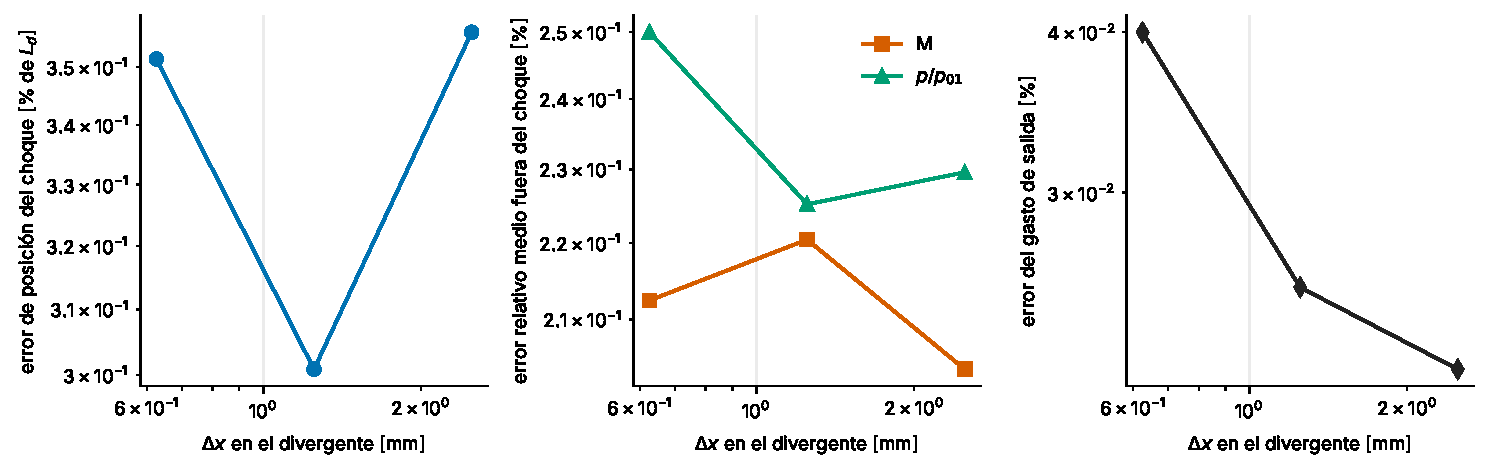
\includegraphics[width=\textwidth]{figuras/convergencia_malla_C.pdf}
  \caption{Estudio de malla del caso C (r1, r2 y r4) en función del tamaño de celda $\Delta x$ en el divergente. Izquierda: error de posición del choque (porcentaje de $L_d$). Centro: error relativo medio de $M$ y $p/p_{01}$ fuera de la zona del choque. Derecha: error del gasto de salida. Los ejes verticales están ampliados: todos los errores son menores de 0.4\,\% de $L_d$, de 0.3\,\% en $M$ y $p/p_{01}$ y de 0.04\,\% en el gasto, sin tendencia monótona al refinar: la sensibilidad a la malla es pequeña, aunque no se demuestra convergencia rigurosa.}
  \label{fig:conv-malla-C}
\end{figure}

\subsection{Sensibilidad al paso de tiempo}
\label{sec:sens-dt}

Las primeras corridas se hicieron con Courant máximo de 0.3 a 0.5, valores habituales en \texttt{rhoCentralFoam}. Con ellos aparecieron discrepancias que no disminuían con el refinamiento de malla, por lo que se repitieron los casos con Courant 0.1. La Tabla~\ref{tab:sens-dt} resume la comparación y la Figura~\ref{fig:sens-dt} muestra su efecto en el perfil del caso C.

\begin{table}[H]
\centering
\caption{Efecto del número de Courant máximo en los resultados (promedio en ventana, secciones).}
\label{tab:sens-dt}
\renewcommand{\arraystretch}{1.2}
\small
\begin{tabular}{llcc}
\toprule
\textbf{Caso (malla)} & \textbf{Magnitud} & \textbf{Courant 0.3--0.5} & \textbf{Courant 0.1} \\
\midrule
S (r2, $p_B=276$ kPa) & Error del gasto & $-13.1$~\% & $-0.08$~\% \\
S (r2, $p_B=276$ kPa) & Pérdida de $p_0$ en la salida & 0.58~\% & 0.03~\% \\
S (r1) & Error medio de $M$ & 1.11~\% & 0.08~\% \\
S (r1) & Error del gasto & $-1.07$~\% & $-0.10$~\% \\
A (r1) & Error medio de $M$ & 0.37~\% & 0.22~\% \\
C (r1) & Error medio de $M$ & 1.22~\% & 0.21~\% \\
C (r1) & Posición del choque $x_s/L_d$ (error) & 0.612 (6.2~\% $L_d$) & 0.677 (0.36~\% $L_d$) \\
C (r2) & Posición del choque $x_s/L_d$ (error) & 0.582 (9.2~\% $L_d$) & 0.676 (0.30~\% $L_d$) \\
C (r4) & Posición del choque $x_s/L_d$ (error) & 0.607 (6.7~\% $L_d$) & 0.677 (0.35~\% $L_d$) \\
\bottomrule
\end{tabular}
\end{table}

\begin{figure}[H]
  \centering
  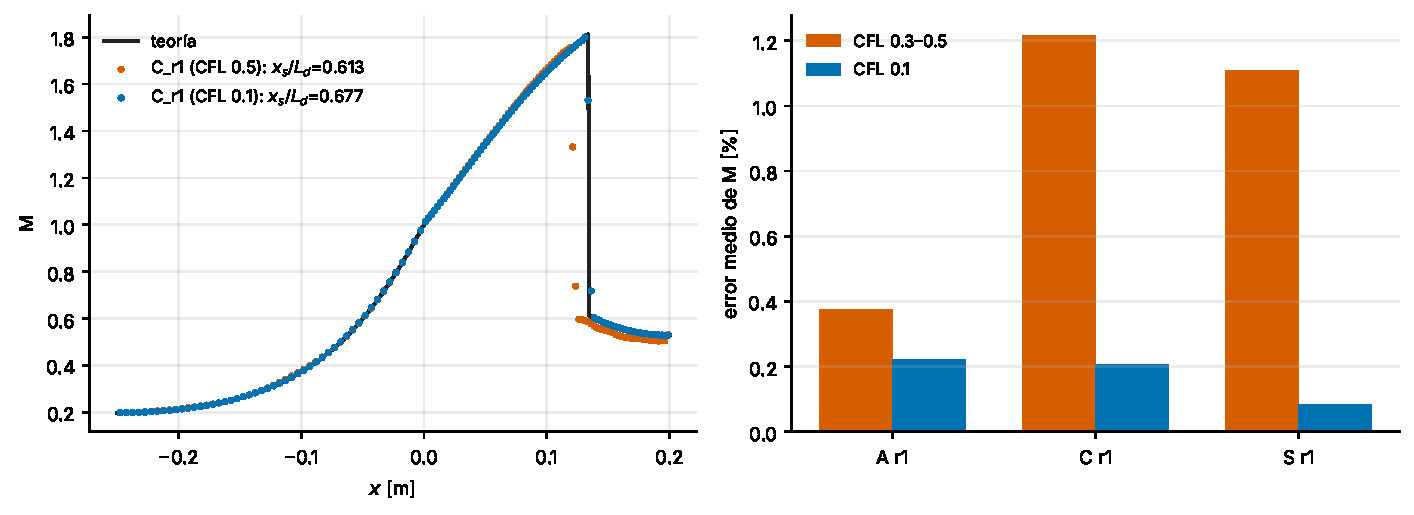
\includegraphics[width=\textwidth]{figuras/sensibilidad_dt.pdf}
  \caption{Sensibilidad al número de CFL. Izquierda: perfil de Mach del caso C (r1) con CFL 0.5 y 0.1; con CFL alto el choque queda desplazado aguas arriba ($x_s/L_d=0.613$) frente al valor con CFL 0.1 (0.677). Derecha: error medio del número de Mach en los casos A, C y S con CFL 0.3--0.5 y con CFL 0.1.}
  \label{fig:sens-dt}
\end{figure}

Los resultados muestran que el paso de tiempo fue el parámetro más influyente del estudio, más que la resolución de la malla:

\begin{itemize}
  \item En el caso S con Courant 0.3, el error del gasto fue de $-1.1$~\% en la malla r1 y de $-13.1$~\% en r2: no disminuyó al refinar la malla. En r2 la presión total cae 0.58~\% entre la entrada y la salida, aunque el flujo no tiene choques ni fricción, es decir, es una pérdida puramente numérica. Como a $M\approx0.35$ el gasto es muy sensible a la presión total disponible, esa pérdida pequeña produce un error de $-13$~\% en el gasto. Con Courant 0.1 la pérdida baja a 0.03~\% y el error del gasto a $-0.08$~\%. Con $p_B=290$ kPa ($M_e=0.22$), con Courant 0.3, el error del gasto fue de $-19.5$~\%, mayor que con 276 kPa ($-13.1$~\%), por lo que se eligió 276 kPa como condición de referencia.
  \item En el caso C, el choque con Courant 0.5 queda entre 6 y 9~\% de $L_d$ aguas arriba de su posición teórica, y esta diferencia no mejora al refinar la malla (de hecho, r2 es el peor). Con Courant 0.1 la posición del choque coincide con la teoría dentro de 0.4~\% de $L_d$ para las tres mallas.
  \item Con Courant 0.1, los resultados de las dos mallas coinciden entre sí y con la teoría; lo que sugiere que buena parte de la diferencia que con Courant alto parecía espacial era de origen temporal.
\end{itemize}

\subsubsection*{Estudio del orden del error respecto al paso de tiempo}

Para comprobar con datos que el efecto se debe al paso de tiempo, y no solo interpretarlo, se repitieron en la malla r1 los casos A, C y S con Courant máximo de 0.2 y 0.05, que junto con las corridas de 0.1, 0.3 y 0.5 permiten ver cómo cambia el error. La Tabla~\ref{tab:orden-courant} y la Figura~\ref{fig:orden-courant} muestran el resultado.

\begin{table}[H]
\centering
\caption{Error en función del Courant máximo (malla r1; promedio en ventana de tiempo). Los guiones indican que ese Courant no se corrió para ese caso (en C se corrió 0.5 y en S y A, 0.3).}
\label{tab:orden-courant}
\small
\renewcommand{\arraystretch}{1.15}
\begin{tabular}{rccccc}
\toprule
 & \multicolumn{2}{c}{Caso S} & \multicolumn{2}{c}{Caso C} & Caso A \\
\cmidrule(lr){2-3}\cmidrule(lr){4-5}\cmidrule(lr){6-6}
Courant & Error $M$ [\%] & Error $\dot m$ [\%] & Error $x_s$ [\% $L_d$] & Error $M$ [\%] & Error $M$ [\%] \\
\midrule
0.05 & 0.051 & 0.069 & 0.356 & 0.203 & 0.223 \\
0.1 & 0.095 & 0.107 & 0.356 & 0.204 & 0.224 \\
0.2 & 0.459 & 0.445 & 0.333 & 0.264 & 0.277 \\
0.3 & 1.109 & 1.069 & -- & -- & 0.358 \\
0.5 & -- & -- & 6.156 & 1.229 & -- \\
\bottomrule
\end{tabular}
\end{table}

\begin{figure}[H]
  \centering
  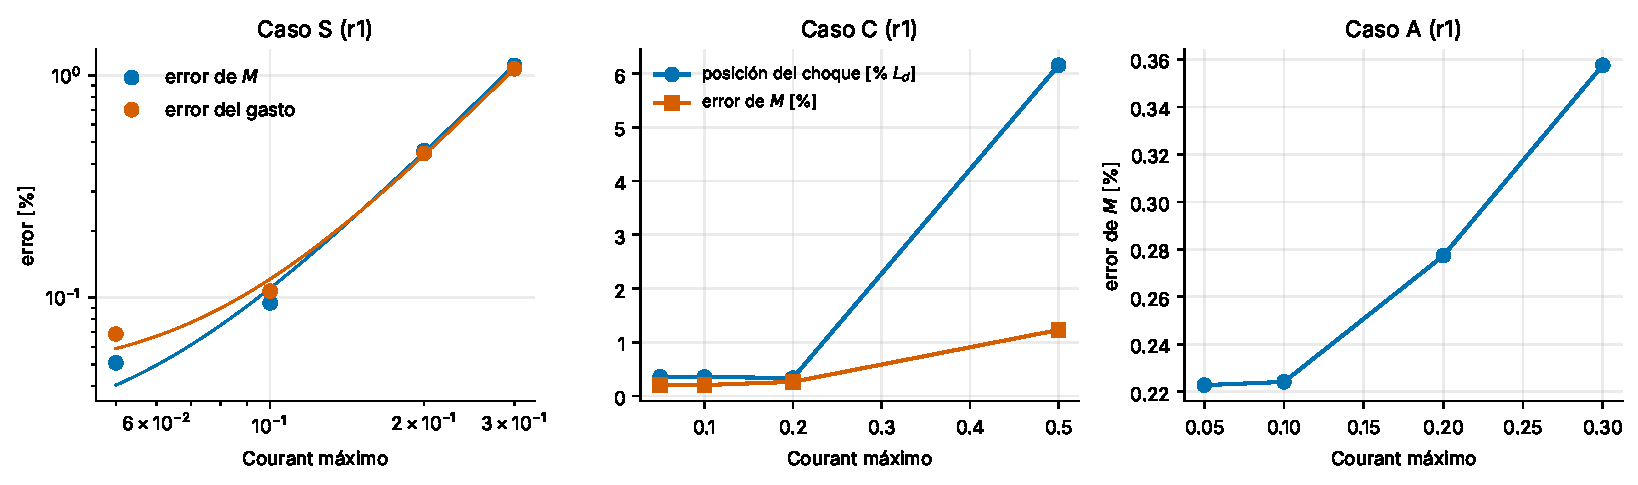
\includegraphics[width=\textwidth]{figuras/orden_courant.pdf}
  \caption{Error en función del Courant máximo (malla r1). Izquierda: caso S (escala logarítmica) con el ajuste $\varepsilon=\varepsilon_0+aC^{p}$. Centro: caso C, posición del choque y error de $M$. Derecha: caso A.}
  \label{fig:orden-courant}
\end{figure}

\begin{itemize}
  \item \textbf{Caso S.} El error disminuye con el Courant más rápido que linealmente: entre 0.3 y 0.1 se reduce unas 12 veces. Un ajuste de la forma $\varepsilon=\varepsilon_0+a\,C^{p}$ a los cuatro puntos da $p\approx2.3$ tanto para el error de $M$ ($\varepsilon_0\approx0.02$~\%) como para el del gasto ($p\approx2.35$, $\varepsilon_0\approx0.04$~\%). Con tres parámetros y cuatro puntos el exponente es solo indicativo, pero muestra una disminución aproximadamente cuadrática hasta un piso de decenas de milésimas de por ciento.
  \item \textbf{Caso C.} La posición del choque casi no cambia entre Courant 0.05 y 0.2 (error de 0.36 a 0.33~\% de $L_d$), pero con 0.5 el error salta a 6.2~\%. No se trata de una dependencia gradual: existe un umbral entre 0.2 y 0.5 (no se corrió 0.3 en este caso) por encima del cual el choque queda mal ubicado. El error medio de $M$ sigue la misma tendencia: 0.20~\% para Courant $\leq0.1$ y 1.23~\% para 0.5.
  \item \textbf{Caso A.} El error de $M$ pasa de 0.36~\% (Courant 0.3) a 0.22~\% (0.1) y ya no cambia al bajar a 0.05: el valor de 0.22~\% es el piso asociado a la diferencia entre el modelo bidimensional y el cuasiunidimensional, no al paso de tiempo.
\end{itemize}

En conjunto, los datos indican que el paso de tiempo controla el error en los tres casos y que existe un valor suficientemente pequeño a partir del cual el error se estabiliza en un piso independiente del paso: $C\leq0.1$ en el caso S (donde el efecto es mayor), y $C\leq0.2$ en C y A. Los pisos (0.02 a 0.04~\% en S, 0.22~\% en A y 0.36~\% de $L_d$ en C) se atribuyen, como hipótesis, a la diferencia entre el modelo bidimensional y el cuasiunidimensional, aunque no se descarta una contribución de la discretización espacial. No se investigó el mecanismo numérico que produce la dependencia casi cuadrática en el caso S; solo se documenta el comportamiento observado.

Por último, se repitió el caso S (r1, Courant 0.1) partiendo de un campo uniforme ($p=p_B=276$ kPa, $T=300$ K, velocidad nula) en vez del campo no uniforme de las corridas de referencia. Con el campo uniforme los errores fueron 0.060~\% en $M$ y $-0.083$~\% en el gasto, contra 0.095~\% y $-0.107$~\% con el campo no uniforme: la diferencia entre ambos es menor que 0.04 puntos porcentuales, por lo que el resultado final no depende de la condición inicial.

Se probaron también otras alternativas para el caso S con Courant 0.3. En la malla r1 (error medio de $M$ de 1.11~\% con la configuración base), el limitador \texttt{Minmod} lo redujo a 0.76~\% y el flujo de Tadmor a 0.69~\%: mejoras moderadas, lejos del 0.09~\% que se obtiene solo al reducir el Courant a 0.1. En la malla r2, una condición de salida \texttt{waveTransmissive} (con longitudes de relajación $l_\infty$ de 0.05, 0.20 y 0.45 m) empeoró el error del gasto a $-45$, $-70$ y $-74$~\%, por lo que se descartó. Esas corridas se listan en el Anexo~\ref{anexo:corridas}.

\subsection{Limitaciones}

\begin{itemize}
  \item El modelo es inviscido y bidimensional; no incluye capa límite ni efectos tridimensionales, por lo que sus resultados deben compararse con el modelo ideal y no con una tobera real.
  \item La teoría cuasiunidimensional supone propiedades uniformes en cada sección; las diferencias mínimas observadas (0.1 a 0.3~\%) incluyen la no uniformidad de la sección, especialmente cerca del choque y en el convergente.
  \item Las ventanas de promedio de las mallas finas son cortas (r4: 0.012--0.02~s) por costo de cómputo; aun así, el criterio de convergencia se cumple.
  \item La ejecución en paralelo con MS-MPI (blueCFD) falló en el equipo utilizado (error 1726), por lo que todas las corridas fueron en serie.
  \item Se estudió el Nivel 1 (casos S, A y C); las condiciones de descarga exterior no forman parte de este reporte.
\end{itemize}

\newpage
\section{Conclusiones}

Se simuló el flujo compresible inviscido en una tobera convergente-divergente plana con $A_e/A_t=1.6$ y se comparó con la teoría cuasiunidimensional que usa el área real $A(x)$. Respecto a los objetivos del estudio:

\begin{enumerate}
  \item \textbf{Regímenes.} Se reprodujeron los tres regímenes del Nivel 1: subsónico no estrangulado ($p_B=276$ kPa, $M_t=0.669$ teórico), supersónico adaptado ($M_e=1.9355$ contra 1.9353) y con choque normal interno ($p_B=200$ kPa).
  \item \textbf{Concordancia con la teoría.} Con Courant 0.1, el error medio del número de Mach fue de 0.08 a 0.22~\%, el de la presión de 0.07 a 0.27~\% y el del gasto másico de 0.02 a 0.10~\%, todos muy por debajo del 10~\%. El balance de masa entre entrada y salida cierra dentro de 0.005~\%. El gasto del caso A (0.17498 kg/s) coincide con el gasto bloqueado teórico (0.17502 kg/s).
  \item \textbf{Choque.} Su posición queda a 0.30--0.36~\% de $L_d$ de la teórica ($x_s/L_d$ de 0.676 contra 0.673), los números de Mach antes y después difieren de la teoría en menos de 1~\% y la relación de presiones totales es 0.810 contra 0.806.
  \item \textbf{Malla.} Con las mallas de 2\,600, 10\,400 y 41\,600 celdas la sensibilidad a la malla es pequeña (errores menores que 0.4~\% de $L_d$ en la posición del choque y 0.04~\% en el gasto), aunque los errores no decrecen de forma sistemática y las ventanas de promedio difieren, por lo que no se demuestra convergencia de malla rigurosa. El error restante puede deberse tanto a la discretización espacial como a la diferencia entre el modelo bidimensional y el cuasiunidimensional; con estos datos no se separan ambas contribuciones.
  \item \textbf{Paso de tiempo.} El número de Courant fue el parámetro más influyente: con 0.3 a 0.5 el gasto subsónico presentó errores de hasta $-13$~\% y el choque se desplazó de 6 a 9~\% de $L_d$; con 0.1 ambos se reducen a los valores reportados arriba (0.02 a 0.10~\% en el gasto y 0.30 a 0.36~\% de $L_d$ en la posición del choque). Un estudio con Courant de 0.05 a 0.5 en la malla r1 muestra que el error disminuye al reducir el paso de tiempo hasta un piso que ya no cambia; en el caso S un ajuste de cuatro puntos da un exponente cercano a 2.3, que es solo indicativo y no establece el orden temporal del método. En flujos de bajo Mach la pérdida numérica de presión total (0.58~\% con Courant 0.3) basta para producir ese error en el gasto.
  \item \textbf{Convergencia.} Todos los casos cumplieron el criterio de cierre definido (cambios entre ventanas menores que 1~\%, balance de masa menor que 1~\% y desplazamiento del choque menor que 0.5~\% de $L_d$).
\end{enumerate}

\textbf{Límites.} El modelo es inviscido y bidimensional, el mecanismo numérico por el que el paso de tiempo afecta el caso S no se investigó, las ventanas de promedio de la malla más fina son cortas y las corridas fueron en serie por una falla de MS-MPI.

\textbf{Mejoras propuestas.} (i) Investigar el mecanismo de la dependencia del error con el paso de tiempo, por ejemplo con un esquema de integración de mayor orden; (ii) repetir el caso S a más valores de contrapresión con Courant 0.1 para trazar la curva de gasto contra $p_B/p_{01}$; (iii) incluir viscosidad y capa límite para comparar con el modelo ideal; (iv) extender el dominio al exterior para estudiar las descargas sobreexpandida y subexpandida.

\newpage
\begin{thebibliography}{99}
\addcontentsline{toc}{section}{Referencias}
\bibitem{anderson2003} Anderson, J.~D., \textit{Modern Compressible Flow: With Historical Perspective}, 3.ª ed., McGraw-Hill, 2003.
\bibitem{anderson2017} Anderson, J.~D., \textit{Fundamentals of Aerodynamics}, 6.ª ed., McGraw-Hill, 2017.
\bibitem{kurganov2000} Kurganov, A. y Tadmor, E., ``New high-resolution central schemes for nonlinear conservation laws and convection--diffusion equations'', \textit{Journal of Computational Physics}, vol.~160, pp.~241--282, 2000.
\bibitem{kurganov2001} Kurganov, A., Noelle, S. y Petrova, G., ``Semidiscrete central-upwind schemes for hyperbolic conservation laws and Hamilton--Jacobi equations'', \textit{SIAM Journal on Scientific Computing}, vol.~23, pp.~707--740, 2001.
\bibitem{greenshields2010} Greenshields, C.~J., Weller, H.~G., Gasparini, L. y Reese, J.~M., ``Implementation of semi-discrete, non-staggered central schemes in a colocated, polyhedral, finite volume framework, for high-speed viscous flows'', \textit{International Journal for Numerical Methods in Fluids}, vol.~63, pp.~1--21, 2010.
\bibitem{vanleer1979} van Leer, B., ``Towards the ultimate conservative difference scheme. V. A second-order sequel to Godunov's method'', \textit{Journal of Computational Physics}, vol.~32, pp.~101--136, 1979.
\bibitem{cfl1928} Courant, R., Friedrichs, K. y Lewy, H., ``Über die partiellen Differenzengleichungen der mathematischen Physik'', \textit{Mathematische Annalen}, vol.~100, pp.~32--74, 1928.
\bibitem{gmsh2009} Geuzaine, C. y Remacle, J.-F., ``Gmsh: A 3-D finite element mesh generator with built-in pre- and post-processing facilities'', \textit{International Journal for Numerical Methods in Engineering}, vol.~79, pp.~1309--1331, 2009.
\bibitem{openfoam} OpenFOAM Foundation, \textit{OpenFOAM v8 User Guide}, \url{https://openfoam.org}.
\bibitem{numpy2020} Harris, C.~R. \textit{et al.}, ``Array programming with NumPy'', \textit{Nature}, vol.~585, pp.~357--362, 2020.
\bibitem{scipy2020} Virtanen, P. \textit{et al.}, ``SciPy 1.0: fundamental algorithms for scientific computing in Python'', \textit{Nature Methods}, vol.~17, pp.~261--272, 2020.
\bibitem{hunter2007} Hunter, J.~D., ``Matplotlib: A 2D graphics environment'', \textit{Computing in Science \& Engineering}, vol.~9, pp.~90--95, 2007.
\end{thebibliography}

\appendix
\section{Tabla de corridas}
\label{anexo:corridas}

\begin{longtable}{p{2.0cm}p{5.0cm}p{0.8cm}p{1.7cm}p{0.8cm}p{0.7cm}p{0.8cm}p{2.5cm}}
\caption{Tabla de corridas. Todas con modelo inviscido compresible (\texttt{rhoCentralFoam}) en dominio interno (semidominio 2D). Las condiciones de salida y de cierre se detallan en la Sección~\ref{sec:metodologia}; $\mathrm{wT}$ = \texttt{waveTransmissive}.}\label{tab:corridas-completa}\\
\toprule
ID & Carpeta & Caso & $p_B$ [kPa] & Malla & CFL & $t_f$ [s] & Papel \\
\midrule
\endfirsthead
\toprule ID & Carpeta & Caso & $p_B$ [kPa] & Malla & CFL & $t_f$ [s] & Papel \\ \midrule
\endhead
\bottomrule
\endfoot
\scriptsize \texttt{S\_\allowbreak r1} & \scriptsize \texttt{caso\_\allowbreak S\_\allowbreak r1\_\allowbreak p276\_\allowbreak co01} & \scriptsize S & \scriptsize 276 & \scriptsize r1 & \scriptsize 0.1 & \scriptsize 0.1 & \scriptsize Referencia \\
\scriptsize \texttt{S\_\allowbreak r2} & \scriptsize \texttt{caso\_\allowbreak S\_\allowbreak r2\_\allowbreak p276\_\allowbreak co01} & \scriptsize S & \scriptsize 276 & \scriptsize r2 & \scriptsize 0.1 & \scriptsize 0.05 & \scriptsize Referencia \\
\scriptsize \texttt{A\_\allowbreak r1} & \scriptsize \texttt{caso\_\allowbreak A\_\allowbreak r1\_\allowbreak co01} & \scriptsize A & \scriptsize -- & \scriptsize r1 & \scriptsize 0.1 & \scriptsize 0.06 & \scriptsize Referencia \\
\scriptsize \texttt{A\_\allowbreak r2} & \scriptsize \texttt{caso\_\allowbreak A\_\allowbreak r2\_\allowbreak co01} & \scriptsize A & \scriptsize -- & \scriptsize r2 & \scriptsize 0.1 & \scriptsize 0.04 & \scriptsize Referencia \\
\scriptsize \texttt{C\_\allowbreak r1} & \scriptsize \texttt{caso\_\allowbreak C\_\allowbreak r1\_\allowbreak co01} & \scriptsize C & \scriptsize 200 & \scriptsize r1 & \scriptsize 0.1 & \scriptsize 0.06 & \scriptsize Referencia, estudio de malla \\
\scriptsize \texttt{C\_\allowbreak r2} & \scriptsize \texttt{caso\_\allowbreak C\_\allowbreak r2\_\allowbreak co01} & \scriptsize C & \scriptsize 200 & \scriptsize r2 & \scriptsize 0.1 & \scriptsize 0.04 & \scriptsize Referencia, estudio de malla \\
\scriptsize \texttt{C\_\allowbreak r4} & \scriptsize \texttt{caso\_\allowbreak C\_\allowbreak r4\_\allowbreak co01} & \scriptsize C & \scriptsize 200 & \scriptsize r4 & \scriptsize 0.1 & \scriptsize 0.02 & \scriptsize Referencia, estudio de malla \\
\scriptsize \texttt{A\_\allowbreak r1\_\allowbreak cfl03} & \scriptsize \texttt{caso\_\allowbreak A\_\allowbreak r1} & \scriptsize A & \scriptsize -- & \scriptsize r1 & \scriptsize 0.3 & \scriptsize 0.1 & \scriptsize Sensibilidad al paso de tiempo \\
\scriptsize \texttt{A\_\allowbreak r2\_\allowbreak cfl03} & \scriptsize \texttt{caso\_\allowbreak A\_\allowbreak r2} & \scriptsize A & \scriptsize -- & \scriptsize r2 & \scriptsize 0.3 & \scriptsize 0.1 & \scriptsize Sensibilidad al paso de tiempo \\
\scriptsize \texttt{C\_\allowbreak r1\_\allowbreak cfl05} & \scriptsize \texttt{caso\_\allowbreak C\_\allowbreak r1} & \scriptsize C & \scriptsize 200 & \scriptsize r1 & \scriptsize 0.5 & \scriptsize 0.1 & \scriptsize Sensibilidad al paso de tiempo \\
\scriptsize \texttt{C\_\allowbreak r2\_\allowbreak cfl05} & \scriptsize \texttt{caso\_\allowbreak C\_\allowbreak r2} & \scriptsize C & \scriptsize 200 & \scriptsize r2 & \scriptsize 0.5 & \scriptsize 0.1 & \scriptsize Sensibilidad al paso de tiempo \\
\scriptsize \texttt{C\_\allowbreak r4\_\allowbreak cfl05} & \scriptsize \texttt{caso\_\allowbreak C\_\allowbreak r4} & \scriptsize C & \scriptsize 200 & \scriptsize r4 & \scriptsize 0.5 & \scriptsize 0.08 & \scriptsize Sensibilidad al paso de tiempo \\
\scriptsize \texttt{S\_\allowbreak r1\_\allowbreak cfl03} & \scriptsize \texttt{caso\_\allowbreak S\_\allowbreak r1\_\allowbreak p276\_\allowbreak base} & \scriptsize S & \scriptsize 276 & \scriptsize r1 & \scriptsize 0.3 & \scriptsize 0.06 & \scriptsize Sensibilidad al paso de tiempo \\
\scriptsize \texttt{S\_\allowbreak r2\_\allowbreak cfl03} & \scriptsize \texttt{caso\_\allowbreak S\_\allowbreak r2\_\allowbreak p276} & \scriptsize S & \scriptsize 276 & \scriptsize r2 & \scriptsize 0.3 & \scriptsize 0.06 & \scriptsize Sensibilidad al paso de tiempo \\
\scriptsize \texttt{S\_\allowbreak r2\_\allowbreak p290} & \scriptsize \texttt{caso\_\allowbreak S\_\allowbreak r2} & \scriptsize S & \scriptsize 290 & \scriptsize r2 & \scriptsize 0.3 & \scriptsize 0.06 & \scriptsize Sensibilidad a la contrapresión \\
\scriptsize \texttt{S\_\allowbreak r2\_\allowbreak p280} & \scriptsize \texttt{caso\_\allowbreak S\_\allowbreak r2\_\allowbreak p280} & \scriptsize S & \scriptsize 280 & \scriptsize r2 & \scriptsize 0.3 & \scriptsize 0.06 & \scriptsize Sensibilidad a la contrapresión \\
\scriptsize \texttt{S\_\allowbreak r2\_\allowbreak p273} & \scriptsize \texttt{caso\_\allowbreak S\_\allowbreak r2\_\allowbreak p273} & \scriptsize S & \scriptsize 273 & \scriptsize r2 & \scriptsize 0.3 & \scriptsize 0.06 & \scriptsize Sensibilidad a la contrapresión \\
\scriptsize \texttt{S\_\allowbreak r1\_\allowbreak minmod} & \scriptsize \texttt{caso\_\allowbreak S\_\allowbreak r1\_\allowbreak p276\_\allowbreak minmod} & \scriptsize S & \scriptsize 276 & \scriptsize r1 & \scriptsize 0.3 & \scriptsize 0.06 & \scriptsize Sensibilidad al limitador \\
\scriptsize \texttt{S\_\allowbreak r1\_\allowbreak tadmor} & \scriptsize \texttt{caso\_\allowbreak S\_\allowbreak r1\_\allowbreak p276\_\allowbreak tadmor} & \scriptsize S & \scriptsize 276 & \scriptsize r1 & \scriptsize 0.3 & \scriptsize 0.06 & \scriptsize Sensibilidad al esquema de flujo \\
\scriptsize \texttt{S\_\allowbreak r2\_\allowbreak wt005} & \scriptsize \texttt{caso\_\allowbreak S\_\allowbreak r2\_\allowbreak p276\_\allowbreak wt005} & \scriptsize S & \scriptsize 276 (wT, $l_\infty$=0.05) & \scriptsize r2 & \scriptsize 0.3 & \scriptsize 0.06 & \scriptsize Condición de salida descartada \\
\scriptsize \texttt{S\_\allowbreak r2\_\allowbreak wt020} & \scriptsize \texttt{caso\_\allowbreak S\_\allowbreak r2\_\allowbreak p276\_\allowbreak wt020} & \scriptsize S & \scriptsize 276 (wT, $l_\infty$=0.20) & \scriptsize r2 & \scriptsize 0.3 & \scriptsize 0.06 & \scriptsize Condición de salida descartada \\
\scriptsize \texttt{S\_\allowbreak r2\_\allowbreak wt045} & \scriptsize \texttt{caso\_\allowbreak S\_\allowbreak r2\_\allowbreak p276\_\allowbreak wt045} & \scriptsize S & \scriptsize 276 (wT, $l_\infty$=0.45) & \scriptsize r2 & \scriptsize 0.3 & \scriptsize 0.06 & \scriptsize Condición de salida descartada \\
\scriptsize \texttt{A\_\allowbreak r1\_\allowbreak cfl02} & \scriptsize \texttt{caso\_\allowbreak dt\_\allowbreak A\_\allowbreak r1\_\allowbreak co02} & \scriptsize A & \scriptsize -- & \scriptsize r1 & \scriptsize 0.2 & \scriptsize 0.06 & \scriptsize Orden del error en el paso de tiempo \\
\scriptsize \texttt{A\_\allowbreak r1\_\allowbreak cfl005} & \scriptsize \texttt{caso\_\allowbreak dt\_\allowbreak A\_\allowbreak r1\_\allowbreak co005} & \scriptsize A & \scriptsize -- & \scriptsize r1 & \scriptsize 0.05 & \scriptsize 0.06 & \scriptsize Orden del error en el paso de tiempo \\
\scriptsize \texttt{C\_\allowbreak r1\_\allowbreak cfl02} & \scriptsize \texttt{caso\_\allowbreak dt\_\allowbreak C\_\allowbreak r1\_\allowbreak co02} & \scriptsize C & \scriptsize 200 & \scriptsize r1 & \scriptsize 0.2 & \scriptsize 0.06 & \scriptsize Orden del error en el paso de tiempo \\
\scriptsize \texttt{C\_\allowbreak r1\_\allowbreak cfl005} & \scriptsize \texttt{caso\_\allowbreak dt\_\allowbreak C\_\allowbreak r1\_\allowbreak co005} & \scriptsize C & \scriptsize 200 & \scriptsize r1 & \scriptsize 0.05 & \scriptsize 0.06 & \scriptsize Orden del error en el paso de tiempo \\
\scriptsize \texttt{S\_\allowbreak r1\_\allowbreak cfl02} & \scriptsize \texttt{caso\_\allowbreak dt\_\allowbreak S\_\allowbreak r1\_\allowbreak co02} & \scriptsize S & \scriptsize 276 & \scriptsize r1 & \scriptsize 0.2 & \scriptsize 0.1 & \scriptsize Orden del error en el paso de tiempo \\
\scriptsize \texttt{S\_\allowbreak r1\_\allowbreak cfl005} & \scriptsize \texttt{caso\_\allowbreak dt\_\allowbreak S\_\allowbreak r1\_\allowbreak co005} & \scriptsize S & \scriptsize 276 & \scriptsize r1 & \scriptsize 0.05 & \scriptsize 0.1 & \scriptsize Orden del error en el paso de tiempo \\
\scriptsize \texttt{S\_\allowbreak r1\_\allowbreak unif} & \scriptsize \texttt{caso\_\allowbreak dt\_\allowbreak S\_\allowbreak r1\_\allowbreak unif} & \scriptsize S & \scriptsize 276 & \scriptsize r1 & \scriptsize 0.1 & \scriptsize 0.1 & \scriptsize Independencia de la condición inicial \\
\end{longtable}


\section{Ubicación de archivos y datos}
\label{anexo:archivos}

El paquete de entrega se organiza como sigue (README en la raíz con las versiones y los pasos para reproducir):

\begin{table}[H]
\centering
\renewcommand{\arraystretch}{1.2}
\small
\begin{tabular}{lp{10cm}}
\toprule
\textbf{Carpeta o archivo} & \textbf{Contenido} \\
\midrule
\texttt{reporte/} & Reporte final (\LaTeX{} y PDF) \\
\texttt{memoria\_calculo/} & Memoria de cálculo (Anexo~\ref{anexo:memoria}): formulación, ramas, procedimiento, cálculo manual y código \\
\texttt{tobera.geo} & Geometría y malla paramétrica de Gmsh (parámetro $r$) \\
\texttt{casos/} & Casos de OpenFOAM (\texttt{0/}, \texttt{constant/}, \texttt{system/}) de cada corrida de la Tabla~\ref{tab:corridas-completa} \\
\texttt{datos/} & Perfiles por sección, historias de gasto y presión de salida (CSV y NPZ) \\
\texttt{scripts/} & Scripts de teoría y posproceso (\texttt{teoria.py}, \texttt{resultados.py}) \\
\texttt{figuras/}, \texttt{tablas/} & Figuras y tablas del reporte \\
\bottomrule
\end{tabular}
\end{table}

\subsection*{Trazabilidad de figuras y tablas}

La Tabla~\ref{tab:trazabilidad} relaciona cada figura y tabla de resultados con el caso, la malla, la ventana de promedio, el script que la produce y el archivo de datos del que sale. Los nombres de caso son los de la Tabla~\ref{tab:corridas-completa}; los scripts están en \texttt{scripts/} y los datos en \texttt{datos/}. Los perfiles y las tablas de errores (\texttt{resultados.py}) usan las ventanas finales de cada caso; el estudio de Courant (\texttt{dtstudy.py}) usa sus propias ventanas, indicadas en la fila correspondiente, y por eso sus valores para el Courant 0.1 pueden diferir ligeramente de los de la Tabla~\ref{tab:errores-perfiles}.

{\scriptsize
\setlength{\tabcolsep}{3pt}
\renewcommand{\arraystretch}{1.15}
\begin{longtable}{p{2.3cm}p{3.3cm}p{2.3cm}p{2.7cm}p{3.7cm}}
\caption{Trazabilidad de figuras y tablas.}\label{tab:trazabilidad}\\
\toprule
\textbf{Elemento} & \textbf{Caso(s)} & \textbf{Ventana [s]} & \textbf{Script} & \textbf{Datos} \\
\midrule
\endfirsthead
\toprule
\textbf{Elemento} & \textbf{Caso(s)} & \textbf{Ventana [s]} & \textbf{Script} & \textbf{Datos} \\
\midrule
\endhead
Fig.~\ref{fig:geometria-mallas} & r1, r2, r4 & -- & \texttt{mallas.py} & \texttt{tobera.geo}, mallas \\
Fig.~\ref{fig:gasto-historias} & A r2, S r2, C r2 (CFL 0.1) & historia completa & \texttt{resultados.py} & \texttt{gastoEntrada/\allowbreak Salida\_\allowbreak *.\allowbreak csv} \\
Fig.~\ref{fig:conv-ventanas} & posición del choque: C r1, r2, r4; gasto: A r1, S r2, C r1 & ventanas de 10 ms (10--60 ms, según la duración) & \texttt{resultados.py} & \texttt{axis\_\allowbreak caso\_\allowbreak *.\allowbreak npz}, \texttt{gasto*\_\allowbreak *.\allowbreak csv} \\
Fig.~\ref{fig:perfiles-S} & S r2 ($p_B=276$ kPa, CFL 0.1) & 0.03--0.05 & \texttt{resultados.py} & \texttt{axis\_\allowbreak caso\_\allowbreak S\_\allowbreak r2\_\allowbreak p276\_\allowbreak co01.npz} \\
Fig.~\ref{fig:mapas-S} & S r2 & campo final & \texttt{resultados.py} & \texttt{axis\_\allowbreak caso\_\allowbreak S\_\allowbreak r2\_\allowbreak p276\_\allowbreak co01.npz} \\
Fig.~\ref{fig:perfiles-A}, \ref{fig:mapas-A} & A r2 (CFL 0.1) & 0.02--0.04 & \texttt{resultados.py} & \texttt{axis\_\allowbreak caso\_\allowbreak A\_\allowbreak r2\_\allowbreak co01.npz} \\
Fig.~\ref{fig:perfiles-C}, \ref{fig:mapas-C} & C r1, r2, r4 (CFL 0.1) & 0.03--0.06, 0.02--0.04, 0.012--0.02 & \texttt{resultados.py} & \texttt{axis\_\allowbreak caso\_\allowbreak C\_\allowbreak r\{1,2,4\}\_\allowbreak co01.npz} \\
Fig.~\ref{fig:conv-malla-C} & C r1, r2, r4 & las de la fila anterior & \texttt{resultados.py} & ídem \\
Fig.~\ref{fig:sens-dt}, Tabla~\ref{tab:sens-dt} & A, C, S r1 y r2; CFL 0.3--0.5 y 0.1 & ventanas de cada corrida & \texttt{resultados.py} & \texttt{axis\_\allowbreak caso\_\allowbreak *.\allowbreak npz} \\
Fig.~\ref{fig:orden-courant}, Tabla~\ref{tab:orden-courant} & A, C, S r1; CFL 0.05, 0.1, 0.2, 0.3, 0.5 & A y C: 0.03--0.06 (0.07--0.10 para 0.3 y 0.5); S: 0.07--0.10 (0.04--0.06 para 0.3) & \texttt{dtstudy.py}, \texttt{orden\_\allowbreak courant.py} & \texttt{dtstudy.json}, \texttt{axis\_\allowbreak caso\_\allowbreak dt\_\allowbreak *.\allowbreak npz} \\
Tablas~\ref{tab:errores-perfiles}, \ref{tab:errores-gasto} & A r1, r2; S r1, r2; C r1, r2, r4 & ventanas finales de cada caso & \texttt{resultados.py} & \texttt{tablas/\allowbreak tabla\_\allowbreak errores\_\allowbreak perfiles.csv} \\
Tablas~\ref{tab:estado-salida}, \ref{tab:estado-salida-err} & A, S, C & ventanas finales & \texttt{resultados.py} & \texttt{tablas/\allowbreak tabla\_\allowbreak estado\_\allowbreak salida.csv} \\
Tablas~\ref{tab:choque-C}, \ref{tab:choque-C-estados} & C r1, r2, r4 & ventanas finales & \texttt{resultados.py} & \texttt{tablas/\allowbreak tabla\_\allowbreak choque\_\allowbreak C.csv} \\
Tabla~\ref{tab:ventanas-eq} & todos los casos finales & dos ventanas de 5 ms al final & \texttt{auditoria.py} & \texttt{axis\_\allowbreak caso\_\allowbreak *.\allowbreak npz}, \texttt{gasto*\_\allowbreak *.\allowbreak csv} \\
Tabla~\ref{tab:corridas-completa} & todas las corridas & -- & -- & \texttt{tablas/\allowbreak tabla\_\allowbreak corridas.csv} \\
Fig.~\ref{fig:geometria_area_real} (geometría $A(x)$) & -- & -- & \texttt{gen\_\allowbreak datos.py} (memoria de cálculo) & \texttt{geometria\_\allowbreak Ax.pdf} \\
\bottomrule
\end{longtable}
}

\section{Tabla de contribuciones}
\label{anexo:contribuciones}

\begin{table}[H]
\centering
\renewcommand{\arraystretch}{1.25}
\small
\begin{tabular}{p{3.6cm}p{5.6cm}p{5.6cm}}
\toprule
\textbf{Actividad} & \textbf{Sandra Valeria Tarango Meléndez (365216)} & \textbf{Karyme Hernández Terán (360725)} \\
\midrule
Definición de geometría y parámetros & Definición final de la geometría (perfil de pared tipo coseno, relaciones de áreas y longitudes) y de los parámetros de entrada ($p_{01}$, $T_{01}$, contrapresiones de los casos S, A y C) & Participó en la definición: revisión de la geometría y búsqueda de referencias para establecer los parámetros \\
Teoría y cálculo analítico & Cálculos finales: comparación de la solución analítica con la simulación (errores, posición del choque, gasto másico) & Toda la parte teórica (flujo cuasiunidimensional, choque normal, ramas de solución), cálculos iniciales y comprobación de cálculos \\
Mallado en Gmsh & \texttt{tobera.geo} paramétrico, tres mallas estructuradas (2\,600, 10\,400 y 41\,600 celdas) y etiquetado de parches & Revisión de los parámetros de malla con apoyo en referencias \\
Configuración y corrida en OpenFOAM & Configuración de \texttt{rhoCentralFoam} (esquemas, fronteras, termodinámica) y corrida de todos los casos, incluidas las pruebas de sensibilidad & Apoyo en la elección de parámetros y condiciones de frontera a partir de la teoría \\
Posproceso, figuras y tablas & Extracción de datos, perfiles por sección, historias de gasto, criterio de convergencia, figuras y tablas de errores & Apoyo en la interpretación teórica de los resultados \\
Redacción del reporte & Parte técnica (simulación, resultados y comparación) & Resto de la redacción \\
Revisión final & Sí & Sí \\
\bottomrule
\end{tabular}
\end{table}

\clearpage
\section{Memoria de cálculo analítico}
\label{anexo:memoria}

Esta memoria desarrolla el modelo analítico cuasiunidimensional que se usa como referencia en el reporte. Sus ecuaciones, ramas y valores son los que se comparan con la simulación en la Sección~\ref{sec:resultados}; el código que los genera es el de la Sección~\ref{m:cod} y está en el paquete de entrega.

\begingroup\small\setlength{\parindent}{0pt}\setlength{\parskip}{0.4em}
% Memoria de calculo analitico (anexo). Generado a partir de memoria_calculo.tex
% ---------- atajos de notación ----------
\newcommand{\ptot}{p_0}\newcommand{\Ttot}{T_0}
\newcommand{\As}{A^{*}}
\newcommand{\dd}{\,\mathrm{d}}
\newcommand{\Msone}{M_{s1}}\newcommand{\Mstwo}{M_{s2}}
\newcommand{\ie}{es decir,\ }

\lstset{basicstyle=\ttfamily\footnotesize,breaklines=true,frame=single,numbers=left,
        numberstyle=\tiny,keywordstyle=\bfseries,language=Python,columns=fullflexible,
        inputencoding=utf8,extendedchars=true,
        literate={á}{{\'a}}1 {é}{{\'e}}1 {í}{{\'i}}1 {ó}{{\'o}}1 {ú}{{\'u}}1 {ñ}{{\~n}}1}

\subsection{Objetivo y alcance}
%=====================================================================
Esta memoria desarrolla, paso a paso y sin saltar álgebra, el modelo analítico
cuasiunidimensional que se usa como referencia para validar las simulaciones CFD
(Gmsh + OpenFOAM-8, solver \texttt{rhoCentralFoam}) de una tobera convergente-divergente
de relación de áreas $A_e/A_t=\ARr$. Se resuelven tres regímenes internos (Nivel~1):

\begin{itemize}[leftmargin=2em]
\item \textbf{S}: subsónico no estrangulado ($M_t<1$ en la garganta),
\item \textbf{A}: supersónico adaptado (garganta sónica, divergente supersónico, $p_e=p_{e,is}$),
\item \textbf{C}: choque normal interno en el divergente.
\end{itemize}

Para cada régimen se obtienen los perfiles $M(x)$, $p(x)/p_{01}$, $T(x)/T_{01}$, el gasto
másico y el estado de salida $(M_e,p_e,T_e,V_e)$ usando la \emph{distribución real} $A(x)$ de la
geometría construida en Gmsh (no una distribución idealizada). En el caso C se obtienen además
$A_s/A_t$, $x_s/L_d$, $M_{s1}$, $M_{s2}$, $p_2/p_1$ y $p_{02}/p_{01}$.

\textbf{Convención de índices.} Subíndice 0: condición de estancamiento (total); subíndice 1:
alimentación (entrada); $t$: garganta geométrica; $e$: salida; $s$: estación del choque; en el choque,
$1$ es aguas arriba y $2$ aguas abajo (se escribe $M_{s1}$, $M_{s2}$ para evitar confusión con el
subíndice de alimentación $p_{01},T_{01}$). El símbolo $A^{*}$ denota el \emph{área crítica}
(el área que tendría la sección si el flujo isentrópico alcanzara $M=1$), que \textbf{no} es
en general igual al área geométrica de garganta $A_t$ (véanse los casos S y C).

%=====================================================================
\subsection{Hipótesis}
%=====================================================================
\begin{enumerate}[label=\textbf{H\arabic*.},leftmargin=2.2em]
\item Flujo \textbf{cuasiunidimensional}: las propiedades dependen sólo de $x$ y el área de la sección
  $A(x)$ varía lentamente. La pendiente máxima de la pared del contorno elegido es pequeña
  (pendiente cero en la garganta y en la salida), lo que hace razonable la hipótesis.
\item Flujo \textbf{estacionario}.
\item Gas \textbf{perfecto} y calóricamente perfecto: $p=\rho R T$, $c_p$ y $\gamma$ constantes;
  aire con $\gamma=\gam$, $R=\Rgas\ \mathrm{J/(kg\,K)}$, $c_p=\gamma R/(\gamma-1)=1004.5\ \mathrm{J/(kg\,K)}$.
\item Flujo \textbf{adiabático e inviscido} (Nivel~1 de la hoja de actividad): paredes impermeables y
  deslizantes, sin capa límite. Entonces $T_0$ es constante a lo largo de todo el flujo, incluso a través del choque.
\item Flujo \textbf{isentrópico} excepto a través del choque normal (caso C); $p_0$ constante antes y
  después del choque, pero con un salto $p_{02}<p_{01}$ en el choque.
\item Dominio \textbf{2D planar}: profundidad $b$ constante en $z$. Con semialtura $h(x)$ y plano de simetría, el área
  de la sección completa es $A(x)=2\,b\,h(x)$; la relación de áreas es entonces
  $A/A_t=h/h_t$ y no depende de $b$. En el modelo numérico se simula la mitad superior con
  $b=\dzz$~m (una celda en $z$).
\item Alimentación de reservorio a $p_{01}=\pu$~kPa, $T_{01}=\Tu$~K, velocidad despreciable en
  el reservorio (parámetros \textbf{provisionales}, a justificar en el reporte).
\end{enumerate}

%=====================================================================
\subsection{Parámetros y geometría real $A(x)$}
%=====================================================================
La geometría de \texttt{tobera.geo} (Gmsh) usa dos tramos con perfil de coseno, con garganta en $x=0$:

\begin{align}
 \text{Convergente } (-L_c\le x\le 0):\quad h(x) &= h_t+\frac{h_i-h_t}{2}\left[1+\cos\!\left(\pi\,\frac{x+L_c}{L_c}\right)\right], \label{m:eq:hconv}\\
 \text{Divergente } (0\le x\le L_d):\quad h(x) &= h_t+\frac{h_e-h_t}{2}\left[1-\cos\!\left(\pi\,\frac{x}{L_d}\right)\right]. \label{m:eq:hdiv}
\end{align}

\textbf{Verificación de los extremos.}
En el convergente: para $x=-L_c$, $\cos(0)=1$ y $h=h_t+(h_i-h_t)=h_i$. Para $x=0$,
$\cos(\pi)=-1$ y $h=h_t$. En el divergente: para $x=0$, $\cos 0=1$ y $h=h_t$; para $x=L_d$, $\cos\pi=-1$
y $h=h_t+(h_e-h_t)=h_e$. La derivada en la garganta es $\mathrm{d}h/\mathrm{d}x=-\tfrac{\pi(h_i-h_t)}{2L_c}\sin(\pi)=0$
por el lado convergente y $\tfrac{\pi(h_e-h_t)}{2L_d}\sin(0)=0$ por el divergente: la pared es suave ($C^1$) en la garganta;
también $\mathrm{d}h/\mathrm{d}x=0$ en $x=L_d$.

\begin{table}[H]\centering
\caption{Parámetros geométricos y de alimentación (provisionales).}\label{m:tab:param}
\begin{tabular}{lcc}\toprule
Parámetro & Símbolo & Valor\\\midrule
Semialtura de garganta & $h_t$ & \hth\ m\\
Semialtura de salida & $h_e=\ARr\,h_t$ & \heh\ m\\
Semialtura de entrada & $h_i=3h_t$ & \hih\ m\\
Longitud del convergente & $L_c$ & \Lcc\ m\\
Longitud del divergente & $L_d$ & \Ldd\ m\\
Relación de áreas asignada & $A_e/A_t=h_e/h_t$ & \ARr\\
Presión total de alimentación & $p_{01}$ & \pu\ kPa\\
Temperatura total de alimentación & $T_{01}$ & \Tu\ K\\
Gas (aire) & $\gamma$, $R$ & \gam, \Rgas\ J/(kg K)\\\bottomrule
\end{tabular}\end{table}

\textbf{Comprobación de la relación de áreas:} $A_e/A_t=h_e/h_t=\heh/\hth=\ARr$. \checkmark

\begin{table}[H]\centering
\caption{Distribución real $A(x)/A_t=h(x)/h_t$ en estaciones seleccionadas.}\label{m:tab:geom}
\begin{tabular}{ccc}
\toprule
$x$ [m] & $h(x)$ [m] & $A/A_t=h/h_t$ \\
\midrule
-0.25 & 0.07500 & 3.0000 \\
-0.20 & 0.07023 & 2.8090 \\
-0.15 & 0.05773 & 2.3090 \\
-0.10 & 0.04227 & 1.6910 \\
-0.05 & 0.02977 & 1.1910 \\
+0.00 & 0.02500 & 1.0000 \\
+0.05 & 0.02720 & 1.0879 \\
+0.10 & 0.03250 & 1.3000 \\
+0.15 & 0.03780 & 1.5121 \\
+0.20 & 0.04000 & 1.6000 \\
\bottomrule
\end{tabular}\end{table}

\begin{figure}[H]\centering
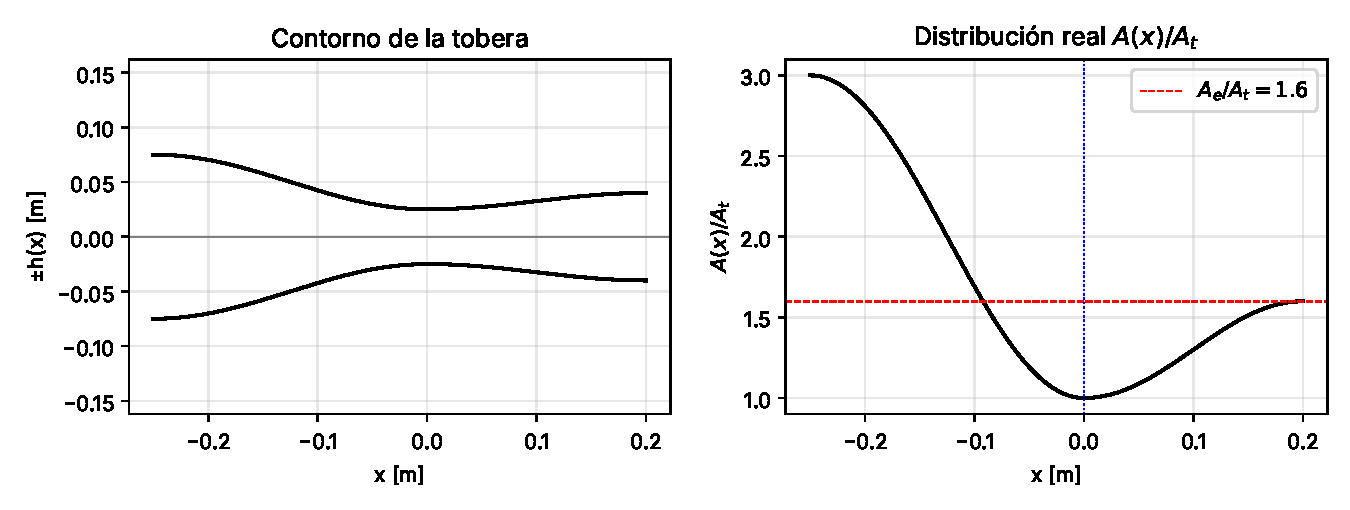
\includegraphics[width=\textwidth]{memoria/figuras/geometria_Ax.pdf}
\caption{Contorno de la tobera (semialtura $\pm h(x)$) y distribución real de áreas $A(x)/A_t$.}
\label{m:fig:geom}\end{figure}

\textbf{Inversa en el divergente.} Para localizar el choque se necesita conocer $x$ a partir de
$A/A_t$. Escribiendo $a\equiv A/A_t=h/h_t$ en \eqref{m:eq:hdiv}:
$a=1+\frac{h_e-h_t}{2h_t}\left[1-\cos(\pi x/L_d)\right]=1+\frac{A_e/A_t-1}{2}\left[1-\cos(\pi x/L_d)\right]$.
Despejando,
\begin{equation}
\cos\!\left(\frac{\pi x}{L_d}\right)=1-\frac{2\,(a-1)}{A_e/A_t-1}
\quad\Longrightarrow\quad
x(a)=\frac{L_d}{\pi}\arccos\!\left[1-\frac{2\,(a-1)}{A_e/A_t-1}\right],\quad 0\le x\le L_d. \label{m:eq:xinv}
\end{equation}
En $[0,L_d]$ la función $\cos(\pi x/L_d)$ es monótona decreciente, por lo que la inversa es única.

%=====================================================================
\subsection{Relaciones isentrópicas}
%=====================================================================
\subsubsection{Temperatura total}
Para un gas calóricamente perfecto, la ecuación de energía de un flujo adiabático estacionario
($h+V^2/2=h_0$ con $h=c_pT$) da
$c_pT+\tfrac12V^2=c_pT_0$. Dividiendo entre $c_pT$ y usando $c_p=\gamma R/(\gamma-1)$ y $a^2=\gamma RT$:
\[
\frac{T_0}{T}=1+\frac{V^2}{2c_pT}=1+\frac{V^2(\gamma-1)}{2\gamma RT}=1+\frac{\gamma-1}{2}M^2,
\]
\begin{equation}
\boxed{\frac{T}{T_0}=\left(1+k\,M^2\right)^{-1},\qquad k\equiv\frac{\gamma-1}{2}=\kk}\label{m:eq:T}
\end{equation}

\subsubsection{Presión y densidad}
En un proceso isentrópico $p/\rho^{\gamma}=\text{cte}$ y $p=\rho RT$, de donde $p\propto T^{\gamma/(\gamma-1)}$ y
$\rho\propto T^{1/(\gamma-1)}$. Con \eqref{m:eq:T}:
\begin{equation}
\boxed{\frac{p}{p_0}=\left(1+kM^2\right)^{-\gamma/(\gamma-1)},\qquad
\frac{\rho}{\rho_0}=\left(1+kM^2\right)^{-1/(\gamma-1)}}\label{m:eq:prho}
\end{equation}
Para $\gamma=\gam$: los exponentes son $-\gamma/(\gamma-1)=-3.5$ y $-1/(\gamma-1)=-2.5$.
Inversa útil (para obtener $M$ a partir de una presión conocida):
\begin{equation}
M=\sqrt{\frac{1}{k}\left[\left(\frac{p_0}{p}\right)^{(\gamma-1)/\gamma}-1\right]}. \label{m:eq:Mdep}
\end{equation}

\subsubsection{Condiciones críticas ($M=1$)}
De \eqref{m:eq:T}--\eqref{m:eq:prho} con $M=1$ y $1+k=(\gamma+1)/2$:
\[
\frac{T^*}{T_0}=\frac{2}{\gamma+1}=0.8333,\qquad
\frac{p^*}{p_0}=\left(\frac{2}{\gamma+1}\right)^{\gamma/(\gamma-1)}=0.5283,\qquad
\frac{\rho^*}{\rho_0}=\left(\frac{2}{\gamma+1}\right)^{1/(\gamma-1)}=0.6339.
\]
Con $T_0=\Tu$~K y $p_0=\pu$~kPa: $\rho_0=p_0/(RT_0)=\rhocero$~kg/m$^3$,
$\rho^*=\rhostar$~kg/m$^3$ y $a^*=\sqrt{2\gamma RT_0/(\gamma+1)}=\astar$~m/s.

%=====================================================================
\subsection{Relación área--Mach}
%=====================================================================
\subsubsection{Derivación}
La conservación de masa para flujo estacionario cuasi-1D es $\dot m=\rho VA=\text{cte}$. Aplicada entre una sección
cualquiera ($M$, $A$) y la sección crítica ($M=1$, $A=\As$) del \emph{mismo} flujo isentrópico:
\[
\rho V A=\rho^*V^*\As
\quad\Longrightarrow\quad
\frac{A}{\As}=\frac{\rho^*V^*}{\rho V}=\frac{\rho^*}{\rho}\cdot\frac{a^*}{M\,a}.
\]
Se expresa cada cociente con \eqref{m:eq:T}--\eqref{m:eq:prho}. Como $\rho_0$ y $T_0$ son iguales en ambas secciones,
\[
\frac{\rho^*}{\rho}=\frac{\rho^*/\rho_0}{\rho/\rho_0}=\frac{\left(1+k\right)^{-1/(\gamma-1)}}{\left(1+kM^2\right)^{-1/(\gamma-1)}}=\left(\frac{1+kM^2}{1+k}\right)^{1/(\gamma-1)},
\qquad
\frac{a^*}{a}=\sqrt{\frac{T^*}{T}}=\left(\frac{1+kM^2}{1+k}\right)^{1/2}.
\]
Multiplicando, los exponentes se suman: $\dfrac{1}{\gamma-1}+\dfrac12=\dfrac{2+(\gamma-1)}{2(\gamma-1)}=\dfrac{\gamma+1}{2(\gamma-1)}$. Por tanto
\begin{equation}
\boxed{\frac{A}{\As}=\frac{1}{M}\left[\frac{1+kM^2}{1+k}\right]^{\frac{\gamma+1}{2(\gamma-1)}}
=\frac{1}{M}\left[\frac{2}{\gamma+1}\left(1+\frac{\gamma-1}{2}M^2\right)\right]^{\frac{\gamma+1}{2(\gamma-1)}}}\label{m:eq:AM}
\end{equation}
(la segunda forma usa $1/(1+k)=2/(\gamma+1)$). Con $\gamma=\gam$ el exponente es $3$.

\subsubsection{Propiedades: dos ramas y mínimo en $M=1$}
Derivando $\ln(A/\As)$ respecto de $M$:
\[
\frac{\dd\ln(A/\As)}{\dd M}=-\frac{1}{M}+\frac{\gamma+1}{2(\gamma-1)}\cdot\frac{2kM}{1+kM^2}
=-\frac1M+\frac{(\gamma+1)M}{2(1+kM^2)}
=\frac{-2(1+kM^2)+(\gamma+1)M^2}{2M(1+kM^2)}.
\]
Como $2k=\gamma-1$, el numerador es $-2-(\gamma-1)M^2+(\gamma+1)M^2=2(M^2-1)$. Entonces
\begin{equation}
\boxed{\frac{\dd(A/\As)}{\dd M}=\frac{A}{\As}\cdot\frac{M^2-1}{M\left(1+kM^2\right)}}\label{m:eq:dAM}
\end{equation}
\textbf{Conclusión:} $A/\As$ decrece para $M<1$, tiene un mínimo igual a $1$ en $M=1$ y crece para $M>1$. Por eso, para un valor dado
$A/\As>1$ existen \emph{dos} soluciones $M$: una subsónica y una supersónica. La rama correcta se elige por la historia del flujo:
subsónica en el convergente; en el divergente, supersónica si la garganta es sónica y no hay choque aguas arriba,
y subsónica después de un choque normal.

\subsubsection{Solución numérica: método de Newton--Raphson}
\eqref{m:eq:AM} es trascendente en $M$ y no se puede despejar en forma cerrada para $\gamma$ general. Se resuelve
$f(M)\equiv A/\As(M)-a=0$ con Newton--Raphson, usando la derivada exacta \eqref{m:eq:dAM}:
\[
M_{n+1}=M_n-\frac{f(M_n)}{f'(M_n)}=M_n-\frac{A/\As(M_n)-a}{\left.A/\As\right|_{M_n}\,(M_n^2-1)/[M_n(1+kM_n^2)]}.
\]
Se detiene cuando $|M_{n+1}-M_n|<10^{-13}$. \textbf{Elección de la semilla:} se toma $M_0=2$ para la rama supersónica y $M_0=0.4$--$0.5$ para la
subsónica, lejos de $M=1$ donde $f'=0$ (allí el método falla porque la derivada se anula).
Newton converge cuadráticamente: el número de cifras correctas se duplica en cada iteración (véanse las tablas).

\subsubsection{Resultado para $A_e/A_t=\ARr$}
\textbf{Rama supersónica} ($M_0=2$, tabla~\ref{m:tab:nsup}) y \textbf{rama subsónica} ($M_0=0.4$, tabla~\ref{m:tab:nsub}):
\[
M_e^{\rm sup}=\MeSup,\qquad M_e^{\rm sub}=\MeSub .
\]
Sustituyendo en \eqref{m:eq:prho} y \eqref{m:eq:T}: $p_e/p_{01}=\peSup$ y $T_e/T_{01}=\TeSup$ en la rama supersónica;
$p_e/p_{01}=\peSubr$ y $T_e/T_{01}=\TeSubr$ en la rama subsónica.

\begin{table}[H]\centering\small
\caption{Newton--Raphson, rama supersónica ($A/\As=\ARr$, $M_0=2$).}\label{m:tab:nsup}
\begin{tabular}{rcccc}
\toprule
$n$ & $M_n$ & $f(M_n)=A/A^*(M_n)-1.6$ & $f'(M_n)$ & $\Delta M_n=-f/f'$ \\
\midrule
0 & 2.0000000000 & 8.750e-02 & 1.406250 & -6.222e-02 \\
1 & 1.9377777778 & 3.276e-03 & 1.301781 & -2.516e-03 \\
2 & 1.9352616065 & 5.189e-06 & 1.297657 & -3.999e-06 \\
3 & 1.9352576078 & 1.309e-11 & 1.297651 & -1.009e-11 \\
4 & 1.9352576078 & 8.882e-16 & 1.297651 & -6.845e-16 \\
\bottomrule
\end{tabular}\end{table}
\begin{table}[H]\centering\small
\caption{Newton--Raphson, rama subsónica ($A/\As=\ARr$, $M_0=0.4$).}\label{m:tab:nsub}
\begin{tabular}{rcccc}
\toprule
$n$ & $M_n$ & $f(M_n)=A/A^*(M_n)-1.6$ & $f'(M_n)$ & $\Delta M_n=-f/f'$ \\
\midrule
0 & 0.4000000000 & -9.860e-03 & -3.235750 & -3.047e-03 \\
1 & 0.3969527930 & 8.541e-05 & -3.292017 & 2.594e-05 \\
2 & 0.3969787361 & 6.284e-09 & -3.291533 & 1.909e-09 \\
3 & 0.3969787380 & -6.661e-16 & -3.291533 & -2.024e-16 \\
\bottomrule
\end{tabular}\end{table}

%=====================================================================
\subsection{Gasto másico bloqueado}
%=====================================================================
Con garganta sónica, el gasto es el de las condiciones críticas: $\dot m=\rho^*a^*A_t$. Usando
$\rho^*=\rho_0\left(\tfrac{2}{\gamma+1}\right)^{1/(\gamma-1)}$, $\rho_0=p_0/(RT_0)$ y
$a^*=\sqrt{\tfrac{2}{\gamma+1}\gamma RT_0}$:
\[
\dot m=A_t\,\frac{p_0}{RT_0}\sqrt{\frac{2\gamma RT_0}{\gamma+1}}\left(\frac{2}{\gamma+1}\right)^{\frac{1}{\gamma-1}}
=A_t\,p_0\sqrt{\frac{\gamma}{RT_0}}\;\sqrt{\frac{2}{\gamma+1}}\left(\frac{2}{\gamma+1}\right)^{\frac{1}{\gamma-1}}.
\]
Los exponentes de $\tfrac{2}{\gamma+1}$ suman $\tfrac12+\tfrac1{\gamma-1}=\tfrac{\gamma+1}{2(\gamma-1)}$:
\begin{equation}
\boxed{\dot m=A_t\,p_0\sqrt{\frac{\gamma}{RT_0}}\left(\frac{2}{\gamma+1}\right)^{\frac{\gamma+1}{2(\gamma-1)}}}\label{m:eq:mdot}
\end{equation}
Numéricamente, $\sqrt{\gamma/(RT_0)}\,(2/(\gamma+1))^{3}=\coefm\ \mathrm{s/m}$, con lo que
\[
\dot m'\equiv\frac{\dot m}{b}=2h_t\,p_{01}\cdot\coefm=\mathbf{\mdotfull}\ \mathrm{kg/(s\,m)}
\quad\text{(por metro de profundidad, tobera completa).}
\]
Para el semidominio simulado ($A_t=h_t\,b$, $b=\dzz$~m): $\dot m=\mdotsemi$~kg/s. \emph{Este es el valor de
referencia para el gasto del CFD en los casos A y C.} Mientras la garganta esté sónica, el gasto no depende de la contrapresión.

%=====================================================================
\subsection{Choque normal}
%=====================================================================
\subsubsection{Ecuaciones}
Sea un choque normal estacionario con estado 1 (aguas arriba, supersónico) y 2 (aguas abajo). Sea $r\equiv\rho_2/\rho_1=V_1/V_2$ (continuidad),
$\Pi\equiv p_2/p_1$. Se usan $a^2=\gamma p/\rho$ y $V_1^2=M_1^2\,\gamma p_1/\rho_1$.

\begin{align}
\text{Continuidad:}&\quad \rho_1V_1=\rho_2V_2\ \Rightarrow\ r=V_1/V_2,\\
\text{Cantidad de movimiento:}&\quad p_1+\rho_1V_1^2=p_2+\rho_2V_2^2,\\
\text{Energía:}&\quad \tfrac{\gamma}{\gamma-1}\tfrac{p_1}{\rho_1}+\tfrac12V_1^2=\tfrac{\gamma}{\gamma-1}\tfrac{p_2}{\rho_2}+\tfrac12V_2^2.
\end{align}

\textbf{Paso 1 (momento).} De la cantidad de movimiento y $V_2=V_1/r$: $p_2-p_1=\rho_1V_1^2(1-1/r)$. Dividiendo entre $p_1$ y usando $\rho_1V_1^2/p_1=\gamma M_1^2$:
\begin{equation}\Pi-1=\gamma M_1^2\left(1-\frac1r\right).\label{m:eq:mom}\end{equation}

\textbf{Paso 2 (energía).} Dividiendo la energía entre $\gamma p_1/\rho_1$ y usando $p_2/\rho_2=(p_1/\rho_1)\,\Pi/r$ y $V_1^2/(\gamma p_1/\rho_1)=M_1^2$:
\[
\frac{1}{\gamma-1}\left(1-\frac{\Pi}{r}\right)+\frac{M_1^2}{2}\left(1-\frac1{r^2}\right)=0
\ \Longrightarrow\
\frac{\Pi}{r}-1=\frac{\gamma-1}{2}M_1^2\left(1-\frac1{r^2}\right).\label{m:eq:en}
\]

\textbf{Paso 3 (eliminar $\Pi$).} Se sustituye \eqref{m:eq:mom} en el lado izquierdo de la ecuación de energía:
\[
\frac{\Pi}{r}-1=\frac1r+\gamma M_1^2\left(\frac1r-\frac1{r^2}\right)-1=-\left(1-\frac1r\right)+\gamma M_1^2\,\frac1r\left(1-\frac1r\right)
=\left(1-\frac1r\right)\left[\frac{\gamma M_1^2}{r}-1\right].
\]
El lado derecho se factoriza como $\tfrac{\gamma-1}{2}M_1^2\left(1-\tfrac1r\right)\left(1+\tfrac1r\right)$. Para un choque no trivial ($r\ne1$) se
\textbf{factoriza y cancela} $(1-1/r)$:
\[
\frac{\gamma M_1^2}{r}-1=\frac{\gamma-1}{2}M_1^2\left(1+\frac1r\right).
\]
Multiplicando por $2r$: $2\gamma M_1^2-2r=(\gamma-1)M_1^2\,r+(\gamma-1)M_1^2$, y agrupando los términos en $r$:
$\left[2\gamma-(\gamma-1)\right]M_1^2=r\left[(\gamma-1)M_1^2+2\right]$, con $2\gamma-(\gamma-1)=\gamma+1$:
\begin{equation}
\boxed{\frac{\rho_2}{\rho_1}=r=\frac{(\gamma+1)M_1^2}{(\gamma-1)M_1^2+2}}\label{m:eq:rho}
\end{equation}

\textbf{Paso 4 (presión).} Sustituyendo \eqref{m:eq:rho} en \eqref{m:eq:mom}, con $1-1/r=\dfrac{r-1}{r}$ y
$r-1=\dfrac{(\gamma+1)M_1^2-(\gamma-1)M_1^2-2}{(\gamma-1)M_1^2+2}=\dfrac{2(M_1^2-1)}{(\gamma-1)M_1^2+2}$:
$\dfrac{r-1}{r}=\dfrac{2(M_1^2-1)}{(\gamma+1)M_1^2}$, y por tanto
\begin{equation}
\boxed{\frac{p_2}{p_1}=\Pi=1+\frac{2\gamma}{\gamma+1}\left(M_1^2-1\right)}\label{m:eq:pres}
\end{equation}

\textbf{Paso 5 (Mach aguas abajo).} $M_2^2=V_2^2\rho_2/(\gamma p_2)=\dfrac{V_1^2/r^2}{\gamma p_1\Pi/\rho_1\cdot r}=\dfrac{M_1^2}{r\,\Pi}$. Multiplicando \eqref{m:eq:rho}
por \eqref{m:eq:pres} (con $\Pi=[2\gamma M_1^2-(\gamma-1)]/(\gamma+1)$):
$r\Pi=\dfrac{M_1^2\,[2\gamma M_1^2-(\gamma-1)]}{(\gamma-1)M_1^2+2}$, de donde
\begin{equation}
\boxed{M_2^2=\frac{(\gamma-1)M_1^2+2}{2\gamma M_1^2-(\gamma-1)}}\label{m:eq:M2}
\end{equation}

\textbf{Paso 6 (temperatura).} De la ley de gas perfecto: $T_2/T_1=\Pi/r$ (y, como $T_0$ no cambia, $T_{02}=T_{01}$).

\textbf{Paso 7 (presión total).} Como $T_0$ es el mismo antes y después, $p_0=p\,(T_0/T)^{\gamma/(\gamma-1)}$ da
$\dfrac{p_{02}}{p_{01}}=\Pi\left(\dfrac{T_1}{T_2}\right)^{\gamma/(\gamma-1)}=\Pi\left(\dfrac r\Pi\right)^{\gamma/(\gamma-1)}$, \ie
\begin{equation}
\boxed{\sigma\equiv\frac{p_{02}}{p_{01}}=r^{\frac{\gamma}{\gamma-1}}\;\Pi^{-\frac{1}{\gamma-1}}
=\left[\frac{(\gamma+1)M_1^2}{(\gamma-1)M_1^2+2}\right]^{\frac{\gamma}{\gamma-1}}\left[\frac{\gamma+1}{2\gamma M_1^2-(\gamma-1)}\right]^{\frac{1}{\gamma-1}}}\label{m:eq:sigma}
\end{equation}
Siempre $\sigma<1$ para $M_1>1$: el choque es irreversible y genera pérdida de presión total.

\subsubsection{Consecuencia para el área crítica}
Como $\dot m=\text{cte}$ a través del choque y $\dot m\propto p_0A^*$ (de \eqref{m:eq:mdot}, con $T_0$ constante), el área crítica
del flujo \emph{aguas abajo} es distinta:
\begin{equation}
p_{01}\,A^*_1=p_{02}\,A^*_2\ \Longrightarrow\ \boxed{A^*_2=\frac{A^*_1}{\sigma}}\ \ (>A^*_1),\qquad A^*_1=A_t\ (\text{garganta sónica}).
\label{m:eq:Astar2}
\end{equation}
Por eso, \textbf{después del choque} la sección de salida se evalúa con $A_e/A^*_2=(A_e/A_t)\,\sigma$ y no con $A_e/A_t$
(esto es lo que la hoja pide: ``utilicen la presión total y el área crítica correspondientes al tramo posterior'').

%=====================================================================
\subsection{Casos}
%=====================================================================
\subsubsection{Rangos de contrapresión}
\textbf{Límite subsónico (garganta justo sónica).} Si la garganta alcanza $M_t=1$ pero el flujo se desacelera en el divergente por la rama subsónica, la salida
tiene $M_e^{\rm sub}=\MeSub$ y $p_B/p_{01}=p/p_0(M_e^{\rm sub})=\pbSubLim$. Para $p_B/p_{01}$ mayor, la garganta no se estrangula.

\textbf{Choque justo en la salida.} El flujo es supersónico en todo el divergente ($M_e=\MeSup$, $p_e/p_{01}=\peSup$), y luego un choque normal en la salida eleva la presión
a $p_B=p_e\,(p_2/p_1)$. Con \eqref{m:eq:pres} a $M_1=\MeSup$: $p_2/p_1=1+\tfrac{2\cdot1.4}{2.4}((\MeSup)^2-1)=\pIIs$, por lo que
$p_B/p_{01}=\peSup\times\pIIs=\pbShockExit$.

\textbf{Adaptado.} $p_B=p_{e,is}$: $p_B/p_{01}=\pbAdapt$.

\begin{table}[H]\centering\small
\caption{Rangos de contrapresión por régimen para $A_e/A_t=\ARr$ y $p_{01}=\pu$~kPa.}\label{m:tab:lim}
\begin{tabular}{llcc}
\toprule
R\'egimen & Condici\'on & $p_B/p_{01}$ & $p_B$ [kPa] \\
\midrule
Subs\'onico (S) & $p_B/p_{01} > 0.8971$ & $>0.8971$ & $>269.1$ \\
Choque interno (C) & $0.5939 < p_B/p_{01} < 0.8971$ & $0.5939$ a $0.8971$ & 178.2 a 269.1 \\
Choque en la salida & --- & 0.5939 & 178.2 \\
Adaptado (A) & $p_B=p_{e,is}$ & 0.1413 & 42.4 \\
Sobreexpandido (O) & $p_{e,is}<p_B<p_{\rm choque\ salida}$ & 0.1413 a 0.5939 & 42.4 a 178.2 \\
Subexpandido (U) & $p_B<p_{e,is}$ & $<0.1413$ & $<42.4$ \\
\bottomrule
\end{tabular}\end{table}

\subsubsection{Caso A: supersónico adaptado}
La garganta es sónica ($A^*=A_t$) y el divergente es supersónico. Con $A(x)/A_t=h(x)/h_t$ se resuelve \eqref{m:eq:AM} para $a=A(x)/A_t$ en cada
estación (rama subsónica para $x<0$, supersónica para $x>0$) y se aplican \eqref{m:eq:prho} y \eqref{m:eq:T}. Estado de salida:
\[
M_e=\MeSup,\quad p_e=\peSup\,p_{01}=\peSupPa\ \text{kPa},\quad T_e=\TeSup\,T_{01}=\TeSupK\ \text{K},
\]
\[
a_e=\sqrt{\gamma RT_e}=\aeSup\ \text{m/s},\quad V_e=M_ea_e=\VeSup\ \text{m/s},\quad \dot m=\mdotsemi\ \text{kg/s (semidominio)}.
\]
La contrapresión para este caso es $p_B=p_e=\peSupPa$~kPa (el CFD se corre con salida libre, sin imponer $p_B$).

\begin{figure}[H]\centering
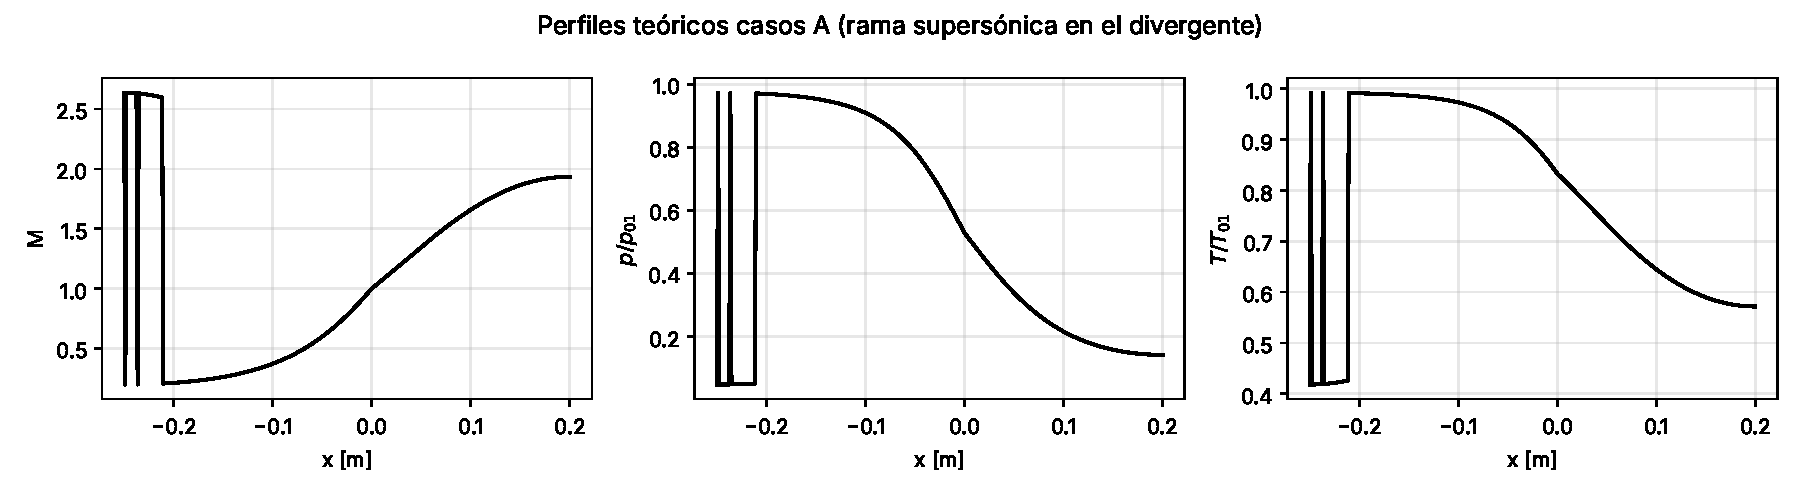
\includegraphics[width=\textwidth]{memoria/figuras/teoria_perfiles_A.pdf}
\caption{Perfiles teóricos del caso A con la $A(x)$ real.}\label{m:fig:perfA}\end{figure}

\subsubsection{Caso S: subsónico no estrangulado}
Con $p_B=\pBS$~kPa ($p_B/p_{01}=\pBSr$, mayor que el límite $\pbSubLim$) la garganta no es sónica, por lo que $A^*\ne A_t$
y hay que \textbf{determinar $A^*$ a partir de la salida}. El flujo es isentrópico y subsónico en toda la tobera y
$p_e=p_B$ (salida subsónica, presión de salida = contrapresión).

\textbf{Paso 1.} Mach de salida con \eqref{m:eq:Mdep}: $M_e=\sqrt{\tfrac{1}{k}\left[(p_{01}/p_B)^{(\gamma-1)/\gamma}-1\right]}=\MeS$.

\textbf{Paso 2.} Cociente de áreas en la salida con \eqref{m:eq:AM}: $A_e/\As=\AeAsS$.

\textbf{Paso 3.} Área crítica relativa a la garganta: $A_t/\As=(A_e/\As)/(A_e/A_t)=\AeAsS/\ARr=\AtAsS$ ($>1$:
la garganta es \emph{más grande} que el área crítica, es decir, subsónica). Equivalentemente $\As/A_t=\AsAtS$.

\textbf{Paso 4.} Mach en la garganta: se resuelve \eqref{m:eq:AM} (rama subsónica) con $a=A_t/\As=\AtAsS$ por Newton (tabla~\ref{m:tab:nS}): $M_t=\MtS<1$.

\textbf{Paso 5.} Gasto: $\dot m=\dot m_{\rm max}\cdot\As/A_t=\mdotsemi\times\AsAtS=\mdotS$~kg/s (semidominio): menor que el bloqueado.

\textbf{Paso 6.} $T_e=T_{01}\,(1+kM_e^2)^{-1}=\TeS$~K y $V_e=M_e\sqrt{\gamma RT_e}=\VeS$~m/s. Los perfiles $M(x)$ salen de resolver \eqref{m:eq:AM}
con $A(x)/\As=(A(x)/A_t)(A_t/\As)=(h/h_t)\,\AtAsS$ en la rama subsónica.

\begin{table}[H]\centering\small
\caption{Newton para $M_t$ del caso S ($A/\As=\AtAsS$, $M_0=0.5$).}\label{m:tab:nS}
\begin{tabular}{rccc}
\toprule
$n$ & $M_n$ & $f(M_n)$ & $\Delta M_n$ \\
\midrule
0 & 0.5000000000 & 2.209e-01 & 1.154e-01 \\
1 & 0.6154235235 & 5.170e-02 & 4.707e-02 \\
2 & 0.6624899194 & 5.426e-03 & 6.198e-03 \\
3 & 0.6686882498 & 8.160e-05 & 9.609e-05 \\
4 & 0.6687843363 & 1.928e-08 & 2.272e-08 \\
5 & 0.6687843590 & 1.110e-15 & 1.308e-15 \\
\bottomrule
\end{tabular}\end{table}

\subsubsection{Caso C: choque normal interno}
\textbf{Datos:} $p_B=\pBC$~kPa ($p_B/p_{01}=\pBCr$, dentro del intervalo $[\pbShockExit,\pbSubLim]$ de choque interno). La garganta es sónica
($A^*_1=A_t$); el choque se ubica donde las condiciones aguas abajo producen exactamente la presión de salida $p_B$.

\textbf{Formulación.} Sea $\Msone$ el Mach justo antes del choque. Aguas abajo el flujo es isentrópico y subsónico hasta la salida, con $p_e=p_B$ (salida subsónica).
La secuencia que liga $\Msone$ con $p_B/p_{01}$ es:
\begin{enumerate}[label=(\roman*)]
\item $\sigma(\Msone)=p_{02}/p_{01}$ con \eqref{m:eq:sigma};
\item área crítica posterior: $A^*_2=A_t/\sigma$ \eqref{m:eq:Astar2}, de modo que $A_e/A^*_2=(A_e/A_t)\,\sigma=\ARr\,\sigma$;
\item $M_e$ subsónico: raíz subsónica de $A/\As(M_e)=\ARr\,\sigma$ \eqref{m:eq:AM};
\item $p_e/p_{01}=\sigma\cdot p/p_0(M_e)$ \eqref{m:eq:prho}, que debe igualar $p_B/p_{01}$.
\end{enumerate}
Así, la incógnita es la raíz de la ecuación escalar
\begin{equation}
F(\Msone)\equiv\sigma(\Msone)\;\frac{p}{p_0}\!\Big|_{M_e(\sigma)}-\frac{p_B}{p_{01}}=0,\qquad 1<\Msone<M_e^{\rm sup}=\MeSup. \label{m:eq:F}
\end{equation}
No tiene solución cerrada (contiene dos inversiones implícitas), por lo que se resuelve numéricamente.

\textbf{Evaluación manual de $F$ en un valor de prueba, $\Msone=\MtrialA$:}
\begin{itemize}[leftmargin=2em]
\item $r=\dfrac{2.4\cdot(\MtrialA)^2}{0.4\cdot(\MtrialA)^2+2}=\rTr$;\quad $\Pi=1+\dfrac{2.8}{2.4}((\MtrialA)^2-1)=\PiTr$;\quad $M_{s2}=\MIITr$.
\item $\sigma=r^{3.5}\,\Pi^{-2.5}=(\rpow)(\Pipow)=\sgTr$.
\item $A_e/A^*_2=\ARr\cdot\sgTr=\AeAdosTr$; raíz subsónica (Newton): $M_e=\MeTr$.
\item $p/p_0=(1+0.2\cdot(\MeTr)^2)^{-3.5}=\prTr$ y $p_e/p_{01}=\sgTr\times\prTr=\pBeTr$.
\item $F=\pBeTr-\pBCr=\FTr>0$.
\end{itemize}
En los extremos del intervalo: $F(1^+)=\FaExt$ y $F(M_e^{\rm sup})=\FbExt$; $F$ cambia de signo y es decreciente
(figura~\ref{m:fig:F}), por lo que existe una única raíz.

\textbf{Método: bisección.} Se elige bisección (confiable y simple de justificar, sin derivadas): partiendo de $[a_0,b_0]=[1^+,M_e^{\rm sup}]$ se toma el punto medio
$m_n=(a_n+b_n)/2$; si $F(m_n)>0$ la raíz está a la derecha ($a_{n+1}=m_n$), si no a la izquierda ($b_{n+1}=m_n$). Cada iteración reduce el intervalo a la mitad y la
iteración termina cuando $b_n-a_n<10^{-12}$ (\nbis\ iteraciones, tabla~\ref{m:tab:bis}). Dentro de cada evaluación de $F$ se resuelve el paso (iii) con Newton.

\begin{figure}[H]\centering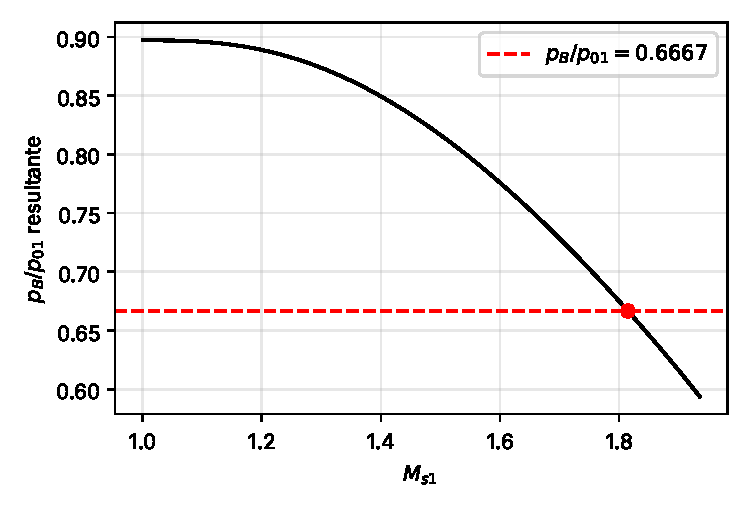
\includegraphics[width=.55\textwidth]{memoria/figuras/F_choque.pdf}
\caption{Presión de salida resultante $p_B/p_{01}$ en función de $M_{s1}$; la intersección con $p_B/p_{01}=\pBCr$ da la solución.}\label{m:fig:F}\end{figure}

\begin{center}\small
\captionof{table}{Bisección de $F(M_{s1})=0$ para el caso C.}\label{m:tab:bis}
\begin{tabular}{rcccc}
\toprule
$n$ & $a_n$ & $b_n$ & $M_{s1}^{(n)}=(a_n+b_n)/2$ & $F(M_{s1}^{(n)})$ \\
\midrule
0 & 1.00000100 & 1.93525761 & 1.46762930 & +1.614e-01 \\
1 & 1.46762930 & 1.93525761 & 1.70144346 & +6.103e-02 \\
2 & 1.70144346 & 1.93525761 & 1.81835053 & -2.033e-03 \\
3 & 1.70144346 & 1.81835053 & 1.75989699 & +3.045e-02 \\
4 & 1.75989699 & 1.81835053 & 1.78912376 & +1.445e-02 \\
5 & 1.78912376 & 1.81835053 & 1.80373715 & +6.265e-03 \\
6 & 1.80373715 & 1.81835053 & 1.81104384 & +2.131e-03 \\
7 & 1.81104384 & 1.81835053 & 1.81469719 & +5.254e-05 \\
8 & 1.81469719 & 1.81835053 & 1.81652386 & -9.892e-04 \\
9 & 1.81469719 & 1.81652386 & 1.81561052 & -4.681e-04 \\
10 & 1.81469719 & 1.81561052 & 1.81515385 & -2.077e-04 \\
11 & 1.81469719 & 1.81515385 & 1.81492552 & -7.758e-05 \\
12 & 1.81469719 & 1.81492552 & 1.81481135 & -1.251e-05 \\
13 & 1.81469719 & 1.81481135 & 1.81475427 & +2.002e-05 \\
14 & 1.81475427 & 1.81481135 & 1.81478281 & +3.752e-06 \\
15 & 1.81478281 & 1.81481135 & 1.81479708 & -4.380e-06 \\
16 & 1.81478281 & 1.81479708 & 1.81478995 & -3.138e-07 \\
17 & 1.81478281 & 1.81478995 & 1.81478638 & +1.719e-06 \\
18 & 1.81478638 & 1.81478995 & 1.81478816 & +7.027e-07 \\
19 & 1.81478816 & 1.81478995 & 1.81478905 & +1.945e-07 \\
20 & 1.81478905 & 1.81478995 & 1.81478950 & -5.967e-08 \\
21 & 1.81478905 & 1.81478950 & 1.81478928 & +6.740e-08 \\
22 & 1.81478928 & 1.81478950 & 1.81478939 & +3.868e-09 \\
23 & 1.81478939 & 1.81478950 & 1.81478944 & -2.790e-08 \\
24 & 1.81478939 & 1.81478944 & 1.81478942 & -1.202e-08 \\
25 & 1.81478939 & 1.81478942 & 1.81478940 & -4.074e-09 \\
26 & 1.81478939 & 1.81478940 & 1.81478940 & -1.027e-10 \\
27 & 1.81478939 & 1.81478940 & 1.81478939 & +1.883e-09 \\
28 & 1.81478939 & 1.81478940 & 1.81478939 & +8.901e-10 \\
29 & 1.81478939 & 1.81478940 & 1.81478940 & +3.937e-10 \\
30 & 1.81478940 & 1.81478940 & 1.81478940 & +1.455e-10 \\
31 & 1.81478940 & 1.81478940 & 1.81478940 & +2.143e-11 \\
32 & 1.81478940 & 1.81478940 & 1.81478940 & -4.062e-11 \\
33 & 1.81478940 & 1.81478940 & 1.81478940 & -9.595e-12 \\
34 & 1.81478940 & 1.81478940 & 1.81478940 & +5.915e-12 \\
35 & 1.81478940 & 1.81478940 & 1.81478940 & -1.840e-12 \\
36 & 1.81478940 & 1.81478940 & 1.81478940 & +2.037e-12 \\
37 & 1.81478940 & 1.81478940 & 1.81478940 & +9.892e-14 \\
38 & 1.81478940 & 1.81478940 & 1.81478940 & -8.706e-13 \\
39 & 1.81478940 & 1.81478940 & 1.81478940 & -3.858e-13 \\
\bottomrule
\end{tabular}\end{center}

\textbf{Resultado.} $\Msone=\MsI$. Con ese valor:
\begin{itemize}[leftmargin=2em]
\item Relaciones del choque: $r=\rrC$; $p_2/p_1=1+\tfrac{2.8}{2.4}(\MsCsq-1)=\pIIpI$; $M_{s2}^2=\numMdos/\denMdos\Rightarrow M_{s2}=\MsII$.
\item $\sigma=p_{02}/p_{01}=\pdospu$ (equivale a $p_{02}=\pdos$~kPa); $A^*_2=A_t/\sigma=\AstarC\,A_t$.
\item Área del choque: $A_s/A_t=A/\As(M_{s1})=\AsAt$.
\item \textbf{Posición del choque} con \eqref{m:eq:xinv}: $\cos(\pi x_s/L_d)=1-2(\AsAt-1)/(\ARr-1)$, y entonces
$x_s=\xsC$~m, es decir $\boxed{x_s/L_d=\xsLd}$ (semialtura de pared $h(x_s)=\hxs$~m).
\item Estados antes/después: $p_{s1}=\pIkPa$~kPa ($p_{s1}/p_{01}=\pIrel$), $T_{s1}=\TIK$~K; $p_{s2}=\pIIkPa$~kPa, $T_{s2}=\TIIK$~K.
\item Salida: $A_e/A^*_2=\AeAstarC$, $M_e=\MeC$, $p_e=\pBC$~kPa (por construcción), $T_e=\TeC$~K, $V_e=\VeC$~m/s.
\end{itemize}

\begin{figure}[H]\centering
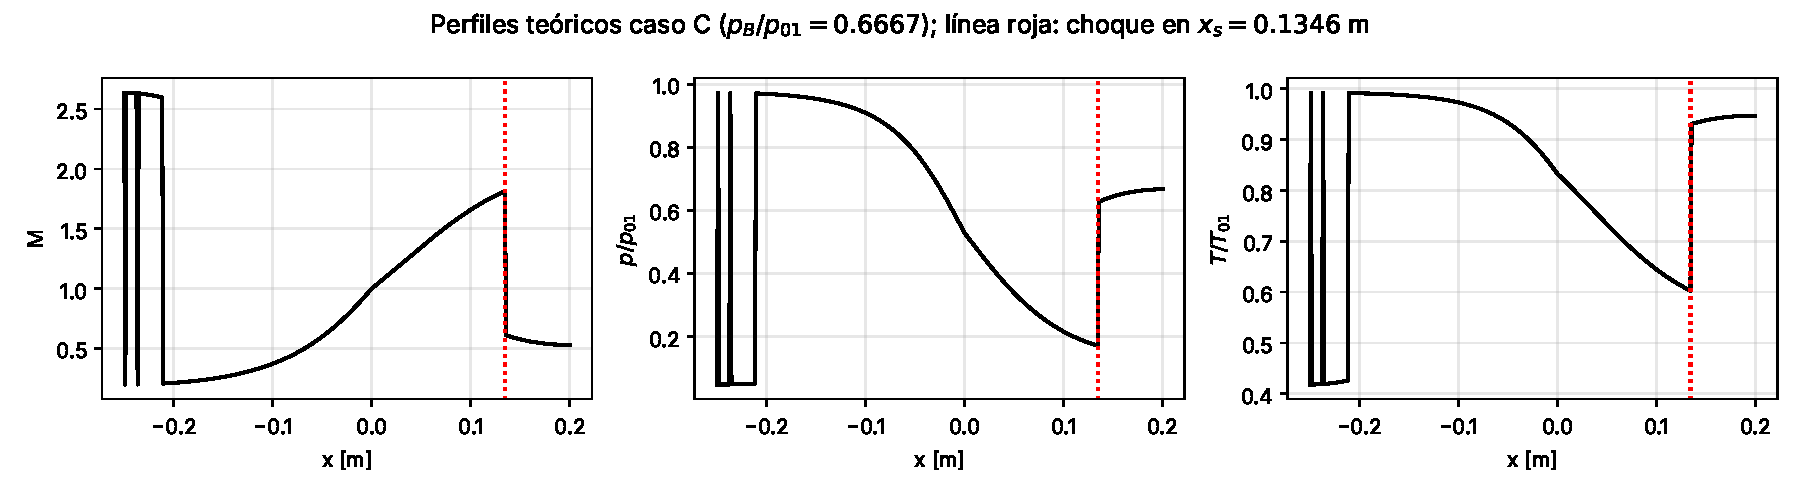
\includegraphics[width=\textwidth]{memoria/figuras/teoria_perfiles_C.pdf}
\caption{Perfiles teóricos del caso C con la $A(x)$ real. El salto en $x_s$ es el choque normal.}\label{m:fig:perfC}\end{figure}

\subsubsection{Cálculo manual completo en una estación del divergente ($x=\xAs$~m, caso A)}
\begin{enumerate}[leftmargin=2em]
\item Altura de pared con \eqref{m:eq:hdiv}: $\cos(\pi x/L_d)=\cos(\pi\cdot\xAs/\Ldd)=\cosA$, por lo que
$h=h_t+\tfrac{h_e-h_t}{2}(1-\cosA)=\hth+\tfrac{\heh-\hth}{2}=\hAs$~m.
\item Cociente de áreas: $A/A_t=\hAs/\hth=\aAs$; garganta sónica $\Rightarrow\As=A_t$, por lo que $A/\As=\aAs$.
\item Se resuelve \eqref{m:eq:AM} (rama supersónica) con Newton, $M_0=1.5$ (tabla~\ref{m:tab:nest}): $M=\MAs$.
\item $p/p_{01}=(1+0.2\cdot(\MAs)^2)^{-3.5}=\pAs$, es decir $p=\pAsPa$~kPa.
\item $T/T_{01}=(1+0.2\cdot(\MAs)^2)^{-1}=\TAs$, es decir $T=\TAsK$~K.
\end{enumerate}
\begin{table}[H]\centering\small
\caption{Newton para la estación $x=\xAs$~m ($A/\As=\aAs$, $M_0=1.5$).}\label{m:tab:nest}
\begin{tabular}{rccc}
\toprule
$n$ & $M_n$ & $f(M_n)$ & $\Delta M_n$ \\
\midrule
0 & 1.5000000000 & -1.238e-01 & 1.832e-01 \\
1 & 1.6831961950 & 2.197e-02 & -2.390e-02 \\
2 & 1.6592927206 & 3.941e-04 & -4.448e-04 \\
3 & 1.6588479422 & 1.353e-07 & -1.528e-07 \\
4 & 1.6588477894 & 1.577e-14 & -1.780e-14 \\
\bottomrule
\end{tabular}\end{table}
Para una estación del convergente, p.~ej.\ $x=\xBs$~m: $h=\hBs$~m, $A/A_t=\aBs$ y la raíz subsónica da $M=\MBs$, $p/p_{01}=\pBs$, $T/T_{01}=\TBs$.

%=====================================================================
\subsection{Definición de métricas de error}
%=====================================================================
Para comparar CFD con teoría se usan las definiciones siguientes (se aplican a magnitudes no nulas):
\begin{align}
\varepsilon_\phi&=\frac{|\phi_{\rm CFD}-\phi_{\rm teo}|}{|\phi_{\rm teo}|}\times100\,\%&&\text{(error relativo puntual o de estación)}\\
\bar\varepsilon_\phi&=\frac1N\sum_{i=1}^{N}\frac{|\phi_{{\rm CFD},i}-\phi_{{\rm teo},i}|}{|\phi_{{\rm teo},i}|}\times100\,\%&&\text{(error medio a lo largo del eje)}\\
\varepsilon_{x_s}&=\frac{|x_{s,\rm CFD}-x_{s,\rm teo}|}{L_d}\times100\,\%&&\text{(error de posición del choque, normalizado con $L_d$)}\\
\delta_{\dot m}&=\frac{\dot m_{\rm sal}-\dot m_{\rm ent}}{\dot m_{\rm ent}}\times100\,\%&&\text{(desbalance de masa)}
\end{align}
La posición del choque en el CFD se define como la coordenada donde el Mach promediado en el tiempo cruza $M=1$ aguas abajo del pico supersónico
(método fijo para todas las mallas); los estados $M_{s1}$, $M_{s2}$, $p_2/p_1$ y $p_{02}/p_{01}$ se miden en estaciones fuera del espesor numérico del choque
(a una distancia de varias celdas a cada lado). Los valores del CFD se promedian en una ventana temporal posterior al arranque, cuyo efecto se evalúa en la sección de sensibilidad temporal.

%=====================================================================

\subsection{Código de la memoria}\label{m:cod}
%=====================================================================
El siguiente módulo implementa exactamente las ecuaciones de las secciones anteriores y es la fuente de todos los números y tablas de este documento.
\lstinputlisting[caption={\texttt{teoria\_tobera.py}}]{memoria/codigo/teoria_tobera.py}

\subsection*{Referencias de la memoria}
\begin{enumerate}[leftmargin=2em]
\item J.~D. Anderson Jr., \emph{Modern Compressible Flow: With Historical Perspective}, 3.ª ed., McGraw-Hill, 2003 (caps.~3--5: ecuaciones isentrópicas, choque normal, flujo en toberas).
\item H.~W. Liepmann y A.~Roshko, \emph{Elements of Gasdynamics}, Dover, 2001.
\item Hoja de actividad y rúbrica, \emph{Proyecto final: simulación de una tobera}, Aerodinámica II (AE604), UACH.
\end{enumerate}

\endgroup

\end{document}
